\documentclass{beamer}
\usetheme{JuanLesPins}

% Document en français, césure, chapitres, etc
\usepackage[T1]{fontenc}
\usepackage[utf8x]{inputenc}
\usepackage[francais]{babel}
\uselanguage{French}
\languagepath{French}

\usepackage[ruled,vlined]{algorithm2e}

\usepackage{hyperref}
\hypersetup{   
	urlcolor=blue,
}

\bibliographystyle{apalike}
\usepackage[round]{natbib}

\usepackage{graphicx}
\usepackage[font=scriptsize]{caption}

\usepackage{verbatim}

% Networks
\def\layersep{2cm}
\usepackage{tikz}
\usepackage{verbatim}
\usetikzlibrary{decorations.pathreplacing}
\usetikzlibrary{decorations.pathreplacing}
\usetikzlibrary{shapes.geometric}

\usepackage{lipsum}

\newcommand\blfootnote[1]{%
	\begingroup
	\renewcommand\thefootnote{}\footnote{#1}%
	\addtocounter{footnote}{-1}%
	\endgroup
}

%Tableaux
\usepackage{array,multirow,makecell}
\usepackage{xcolor,colortbl}
\usepackage{booktabs} 
\definecolor{Gray}{gray}{0.85}
\newcolumntype{a}{>{\columncolor{white}}c}

 \newcommand{\PLH}{{\mkern-2mu\times\mkern-2mu}}

\AtBeginSection[]{
	\begin{frame}
		\vfill
		\centering
		\begin{beamercolorbox}[sep=8pt,center,shadow=true,rounded=true]{title}
			\usebeamerfont{title}\insertsectionhead\par%
		\end{beamercolorbox}
		\vfill
	\end{frame}
}


\title{Détection d’anomalies basée sur les représentations latentes d’un autoencodeur variationnel}
\subtitle{Résumé de mon mémoire de maîtrise}
\author{Stéphane Caron}
\institute{Université Laval}
\date{\today}

\begin{document}
	
	\begin{frame}
		\titlepage
	\end{frame}

	\begin{frame}
		\frametitle{Contenu}
		\tableofcontents
	\end{frame}


	\begin{frame}
		\frametitle{Contexte}
		
		\begin{itemize}
			\item Établissement: Université Laval
			\item Programme: Maîtrise en statistique avec mémoire
			\item Directeur: Thierry Duchesne, Professeur titulaire
			\item Co-directeur: François-Michel De Rainville, Ph.D.
			\item Conseiller en recherche: Samuel Perreault, Ph.D.
		\end{itemize}
	\end{frame}

	\section{Introduction}
	
	\begin{frame}
		\frametitle{Introduction}
		\centering
		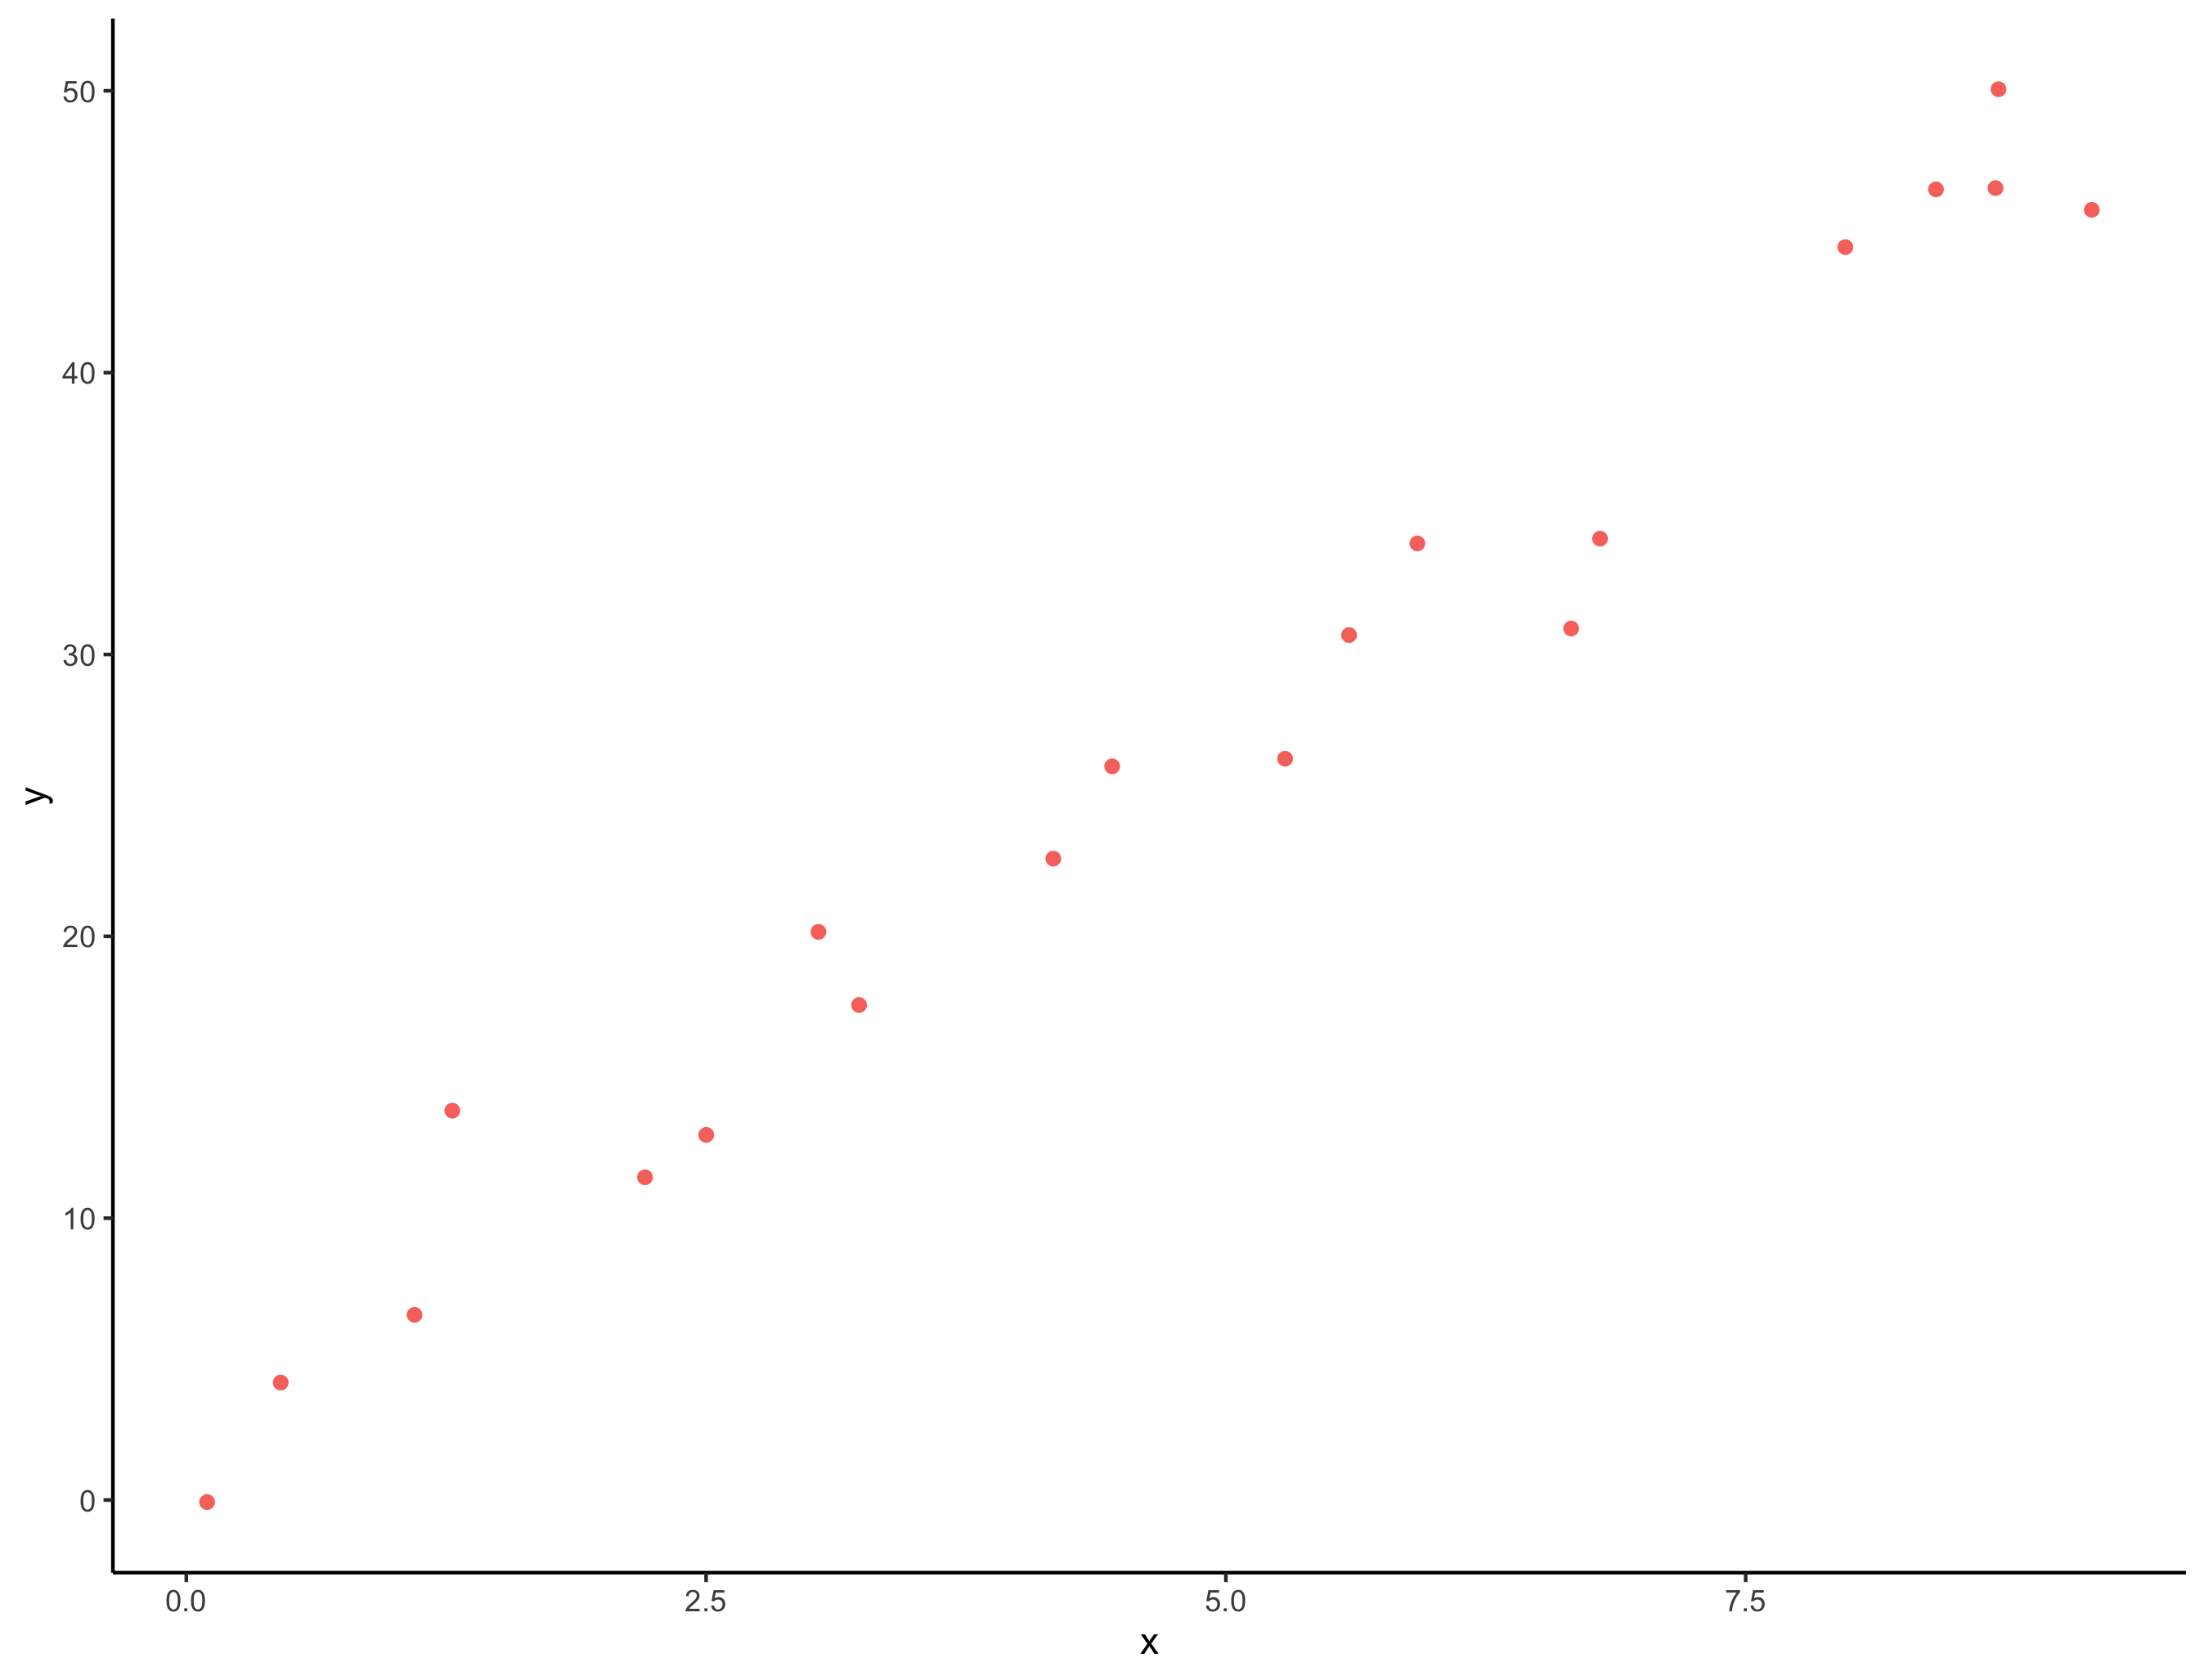
\includegraphics[width=8cm]{images/plot1}
		\blfootnote{Données tirées de \url{https://online.stat.psu.edu/stat462/node/170/}}
	\end{frame}

	\begin{frame}
		\frametitle{Introduction}
		\centering
		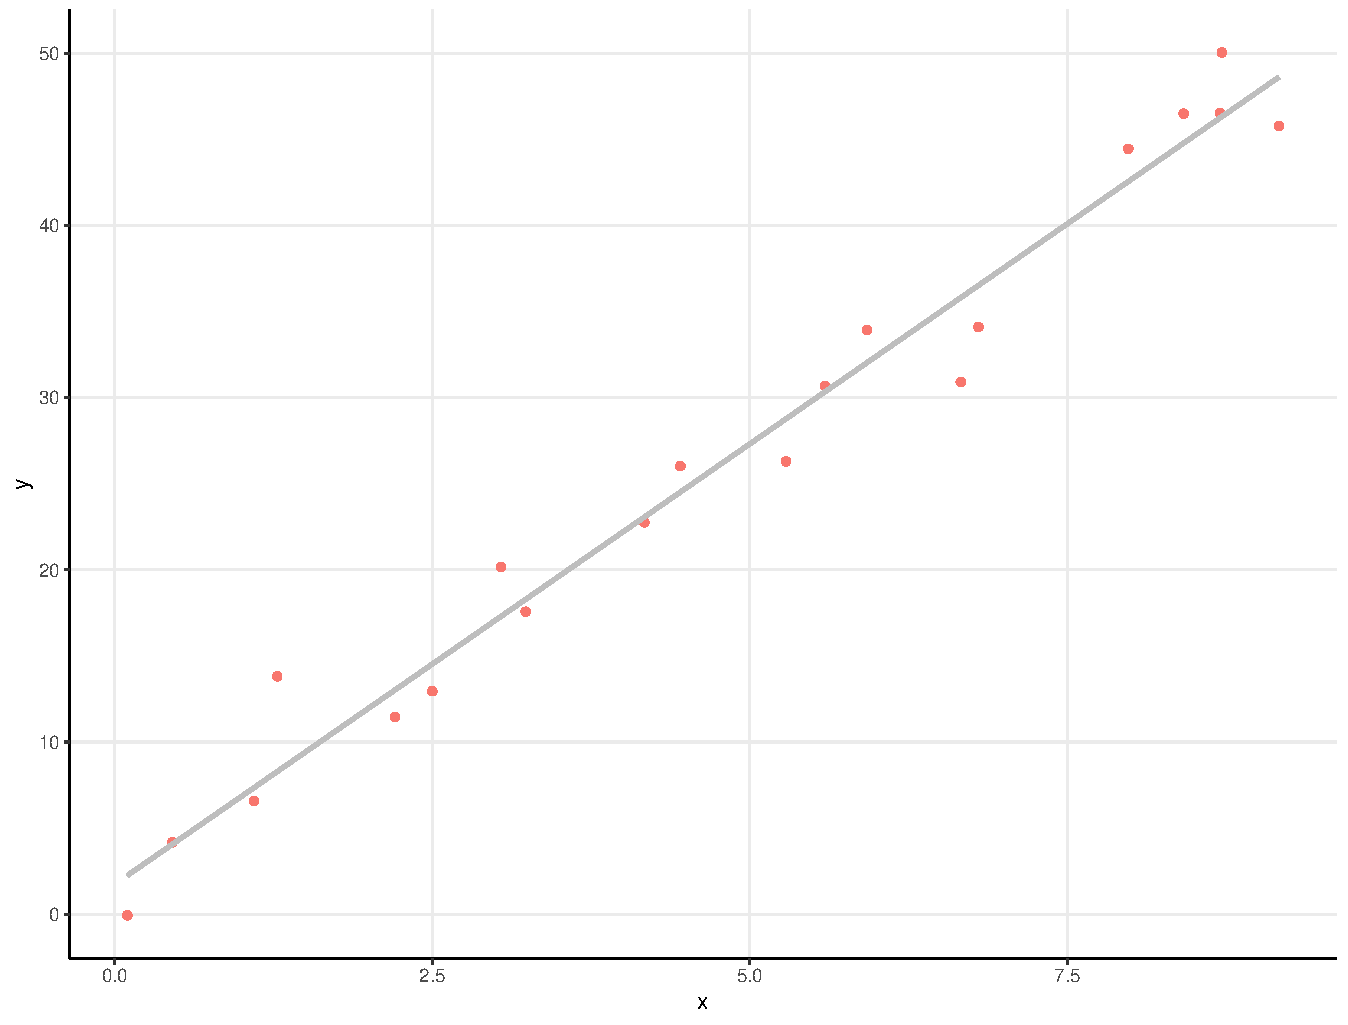
\includegraphics[width=8cm]{images/plot2}
	\end{frame}
	
	\begin{frame}
		\frametitle{Introduction}
		{\footnotesize \verbatiminput{images/lm1.txt}}
	\end{frame}

	\begin{frame}
		\frametitle{Introduction}
		\centering
		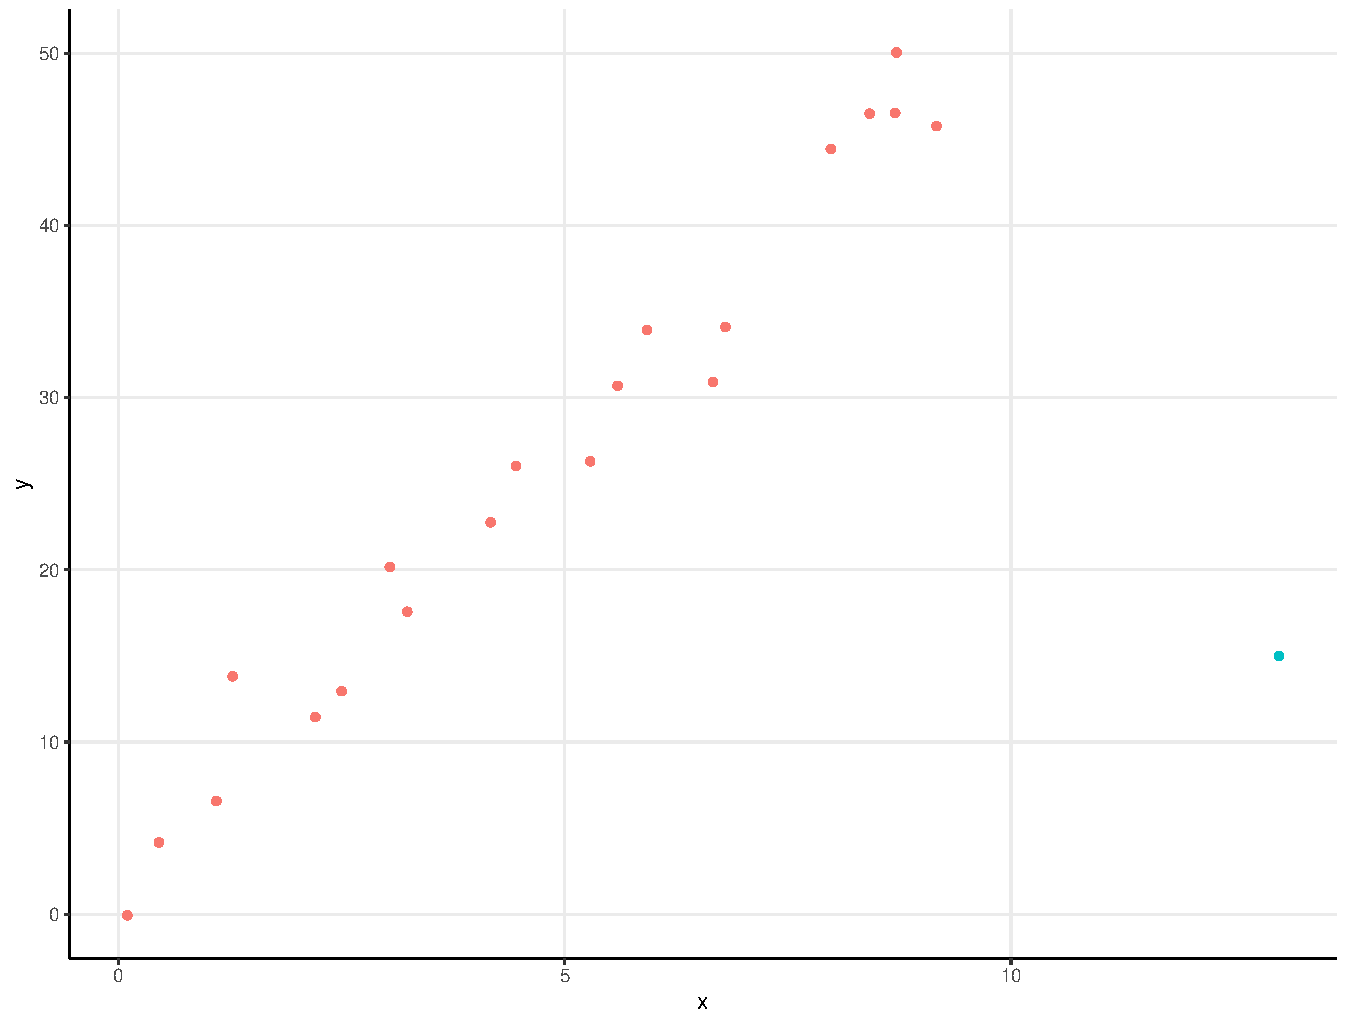
\includegraphics[width=8cm]{images/plot3}
	\end{frame}
	
	\begin{frame}
		\frametitle{Introduction}
		\centering
		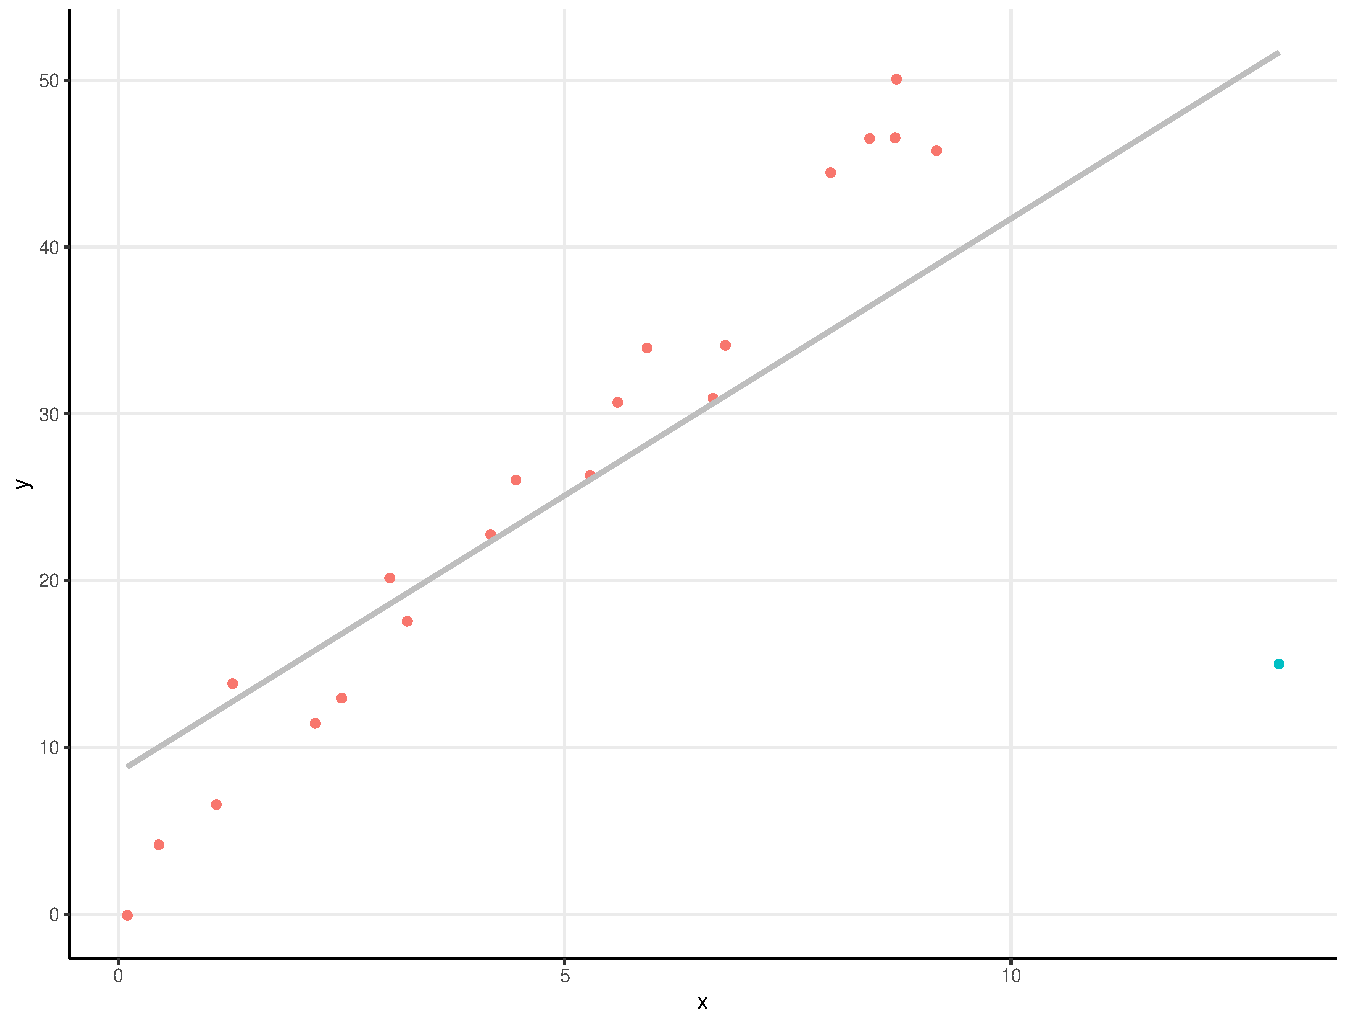
\includegraphics[width=8cm]{images/plot4}
	\end{frame}
	
	\begin{frame}
		\frametitle{Introduction}
		{\footnotesize \verbatiminput{images/lm2.txt}}
	\end{frame}
	
	\section{Mise en contexte}
	
	\begin{frame}
		\frametitle{L'importance du modèle}
		Le choix du modèle est crucial, car si celui-ci ne s’ajuste pas bien aux données, il pourrait nous induire en erreur sur "l’anormalité" d’une observation.
		\begin{figure}
			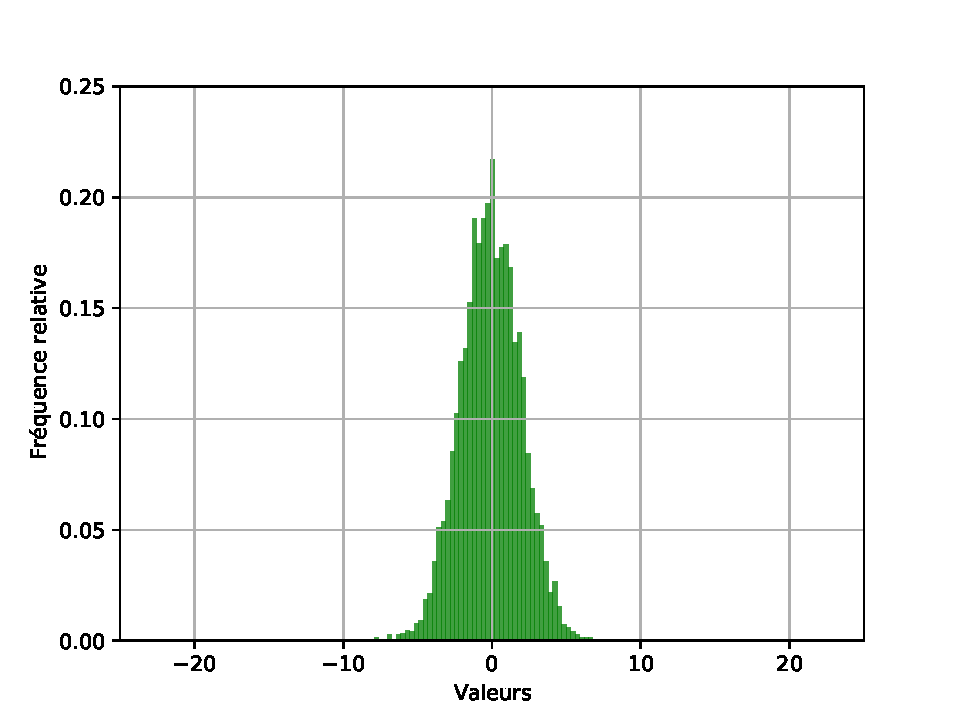
\includegraphics[width=5cm]{../rapports/images/histogram-normal-ztest}
			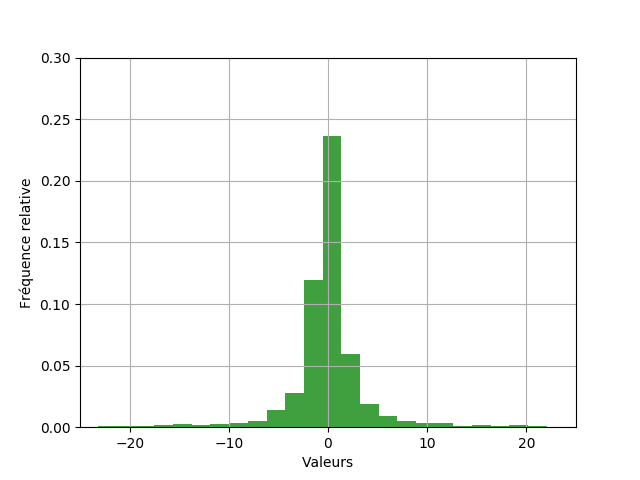
\includegraphics[width=5cm]{../rapports/images/histogram-cauchy-ztest}
			\caption{Distribution de 5000 simulations d'une loi normale (gauche) et d'une loi standard Cauchy (droite).}
		\end{figure}
	
	\end{frame}

	\subsection{Méthodes de détections d'anomalies}
	
	\begin{frame}
		\frametitle{Approches de détection d'anomalies}
		Il est possible définir 4 catégories d'approches \citep{10.5555/3086742}:
		\begin{itemize}
			\item Analyse des valeurs extrêmes
			\item Les modèles probabilistes
			\item Les modèles linéaires et non-linéaires
			\item Les méthodes basées sur les distances
		\end{itemize}
	\end{frame}

	\subsection{Les autoencodeurs}
	
	\begin{frame}
		\frametitle{Autoencodeurs}
		Un autoencodeur est un réseau de neurones qui a comme objectif d’apprendre une représentation intermédiaire d’une entrée de manière non-supervisée \citep{Goodfellow-et-al-2016}.
	\end{frame}

	\begin{frame}
		\frametitle{Autoencodeurs}
		\begin{itemize}
			\item On apprend à encoder ($q$) et décoder ($p$) des observations $x$ de dimensions $D$.
			\item Les représentations latentes $z$, de dimensions $m$, sont généralement de complexité moindre que l'entrée $x$ ($m << D$).
			\item Notations: l'encoder $p$ est une fonction déterministe qui encode l'entrée $x$ ($q(x) = z$), le décodeur est une fonction déterministe qui permet de retrouver les dimensions initiales ($p(z) = \hat{x}$).
		\end{itemize}
	\end{frame}

	\begin{frame}
		\frametitle{Autoencodeurs}
		\begin{figure}[h]
			\centering
			\begin{tikzpicture}[shorten >=1pt,draw=black!50, node distance=\layersep, square/.style={regular polygon,regular polygon sides=4}]
				\tikzstyle{every pin edge}=[<-,shorten <=1pt]
				\tikzstyle{neuron}=[square,fill=black!25,minimum size=17pt,inner sep=0pt]
				\tikzstyle{input neuron}=[neuron, fill=green!50];
				\tikzstyle{output neuron}=[neuron, fill=red!50];
				\tikzstyle{hidden neuron1}=[neuron, fill=blue!50];
				\tikzstyle{hidden neuron2}=[neuron, fill=blue!50];
				\tikzstyle{hidden rep}=[neuron, fill=yellow!50];
				\tikzstyle{annot} = [text width=4em, text centered]
				
				% Draw the input layer nodes
				\foreach \name / \y in {1,...,4}
				% This is the same as writing \foreach \name / \y in {1/1,2/2,3/3,4/4}
				\node[input neuron] (I-\name) at (0,-\y) {};
				
				% Draw the hidden layer nodes n.1
				\foreach \name / \y in {1,...,2}
				\path[yshift=-1cm]
				node[hidden neuron1] (H1-\name) at (\layersep,-\y cm) {};
				
				% Draw the encoded representation
				\foreach \name / \y in {1,...,1}
				\path[yshift=-1.5cm]
				node[hidden rep] (R-\name) at (2 * \layersep,-\y cm) {};
				
				% Draw the hidden layer nodes n.2
				\foreach \name / \y in {1,...,2}
				\path[yshift=-1cm]
				node[hidden neuron1] (H2-\name) at (3 * \layersep,-\y cm) {};
				
				% Draw the output layer
				\foreach \name / \y in {1,...,4}
				% This is the same as writing \foreach \name / \y in {1/1,2/2,3/3,4/4}
				\node[output neuron] (O-\name) at (4 * \layersep,-\y cm) {};
				
				% Connect input
				\foreach \source in {1,...,4}
				\foreach \dest in {1,...,2}
				\path (I-\source) edge (H1-\dest);
				
				% Connect representation
				\foreach \source in {1,...,2}
				\foreach \dest in {1,...,1}
				\path (H1-\source) edge (R-\dest);
				
				\foreach \source in {1,...,1}
				\foreach \dest in {1,...,2}
				\path (R-\source) edge (H2-\dest);
				
				% Connect outputs
				\foreach \source in {1,...,2}
				\foreach \dest in {1,...,4}
				\path (H2-\source) edge (O-\dest);
				
				% Annotate the layers
				\node[annot,above of=I-1, node distance=1cm][text width=6em] (hl) {Couche d'entrée ($x$)};
				\node[annot,above of=R-1, node distance=2.5cm][text width=8em] (hl) {Représentation \\ latente ($z$)};
				\node[annot,above of=O-1, node distance=1cm][text width=6em] (hl) {Couche de sortie ($\hat{x}$)};
				
				\draw [decorate,decoration={brace,mirror,amplitude=15pt},xshift=-4pt,yshift=-2cm]
				(0,-2.5) -- (4,-2.5) node [black,midway,yshift=-3em] 
				{\footnotesize encodeur: $q_{\theta}(x)$};
				\draw [decorate,decoration={brace,mirror,amplitude=15pt},xshift=4pt,yshift=-2cm]
				(4,-2.5) -- (8,-2.5) node [black,midway,yshift=-3em] 
				{\footnotesize décodeur: $p_{\phi}(z)$};
				
			\end{tikzpicture}
			\caption{Exemple illustrant la structure de base d'un autoencodeur.}
		\end{figure}
	\end{frame}

	\begin{frame}
		\frametitle{Optimisation d'un autoencodeur}
		Les paramètres de l'autoencodeur sont généralement optimisés par descente du gradient sur la fonction de perte.
		\begin{itemize}
			\item $\hat{x} = p_{\phi}(q_{\theta}(x))$
			\item $L(x, \hat{x}) = L(x, p_{\phi}(q_{\theta}(x)))$
			\item $\Theta = \{\theta, \phi\}$
			\item $\Theta^{'} \leftarrow \Theta-\epsilon*\frac{\partial L}{\partial\Theta}$, où $\epsilon$ est le taux d'apprentissage
		\end{itemize}
		 
	\end{frame}

	\subsection{Les autoencodeurs variationnels}	
	
	\begin{frame}
		\frametitle{Autoencodeurs variationnels (VAE)}
		Les VAE \citep{kingma2013autoencoding} sont similaires aux AE par rapport au concept d'encodage/décodage, mais ils ont une notion probabiliste additionnelle qui les différencient.
		
		\begin{itemize}
			\item On souhaite avoir un \textit{a priori} sur $z$
			\item $z$ est donc définie de manière continue et non discrète
			\item $p(z) \sim N(0,I)$
			\item $q_{\theta}(z|x) \sim N(\boldsymbol{\mu}, \boldsymbol{\sigma})$
			\item Les paramètres $\boldsymbol{\mu}$ et $\boldsymbol{\sigma}$ sont définis par les couches du réseau précédents la représentation $z$
		\end{itemize}
	\end{frame}

	\begin{frame}
		\frametitle{Autoencodeurs variationnels (VAE)}
		\begin{figure}[ht]
			\centering
			\begin{tikzpicture}[shorten >=1pt,draw=black!50, node distance=\layersep, square/.style={regular polygon,regular polygon sides=4}]
				\tikzstyle{every pin edge}=[<-,shorten <=1pt]
				\tikzstyle{neuron}=[square,fill=black!25,minimum size=17pt,inner sep=0pt]
				\tikzstyle{input neuron}=[neuron, fill=blue!50];
				\tikzstyle{output neuron}=[neuron, fill=blue!50];
				\tikzstyle{hidden neuron1}=[neuron, fill=blue!50];
				\tikzstyle{hidden neuron2}=[neuron, fill=blue!50];
				\tikzstyle{sample rep}=[neuron, fill=yellow!50];
				\tikzstyle{hidden rep}=[neuron, fill=red!50];
				\tikzstyle{annot} = [text width=4em, text centered]
				
				% Draw the input layer nodes
				\foreach \name / \y in {1,...,4}
				% This is the same as writing \foreach \name / \y in {1/1,2/2,3/3,4/4}
				\node[input neuron] (I-\name) at (0,-\y) {};
				
				% Draw the hidden layer nodes n.1
				\foreach \name / \y in {1,...,3}
				\path[yshift=-0.5cm]
				node[hidden neuron1] (H1-\name) at (\layersep,-\y cm) {};
				
				% Draw the mu and sigma layers
				\foreach \name / \y in {1,...,2}
				\path[yshift=-1cm]
				node[hidden rep] (R-\name) at (2 * \layersep,-\y cm) {};
				
				% Draw the encoded representation
				\foreach \name / \y in {1,...,1}
				\path[yshift=-1.5cm]
				node[sample rep] (S-\name) at (3 * \layersep,-\y cm) {};
				
				% Draw the hidden layer nodes n.2
				\foreach \name / \y in {1,...,3}
				\path[yshift=-0.5cm]
				node[hidden neuron1] (H2-\name) at (4 * \layersep,-\y cm) {};
				
				% Draw the output layer
				\foreach \name / \y in {1,...,4}
				% This is the same as writing \foreach \name / \y in {1/1,2/2,3/3,4/4}
				\node[output neuron] (O-\name) at (5 * \layersep,-\y cm) {};
				
				% Connect input
				\foreach \source in {1,...,4}
				\foreach \dest in {1,...,3}
				\path (I-\source) edge (H1-\dest);
				
				% Connect hidden 1 with mu and sigma
				\foreach \source in {1,...,3}
				\foreach \dest in {1,...,2}
				\path (H1-\source) edge (R-\dest);
				
				% Connect representation
				\foreach \source in {1,...,2}
				\foreach \dest in {1,...,1}
				\path (R-\source) edge (S-\dest);
				
				\foreach \source in {1,...,1}
				\foreach \dest in {1,...,3}
				\path (S-\source) edge (H2-\dest);
				
				% Connect outputs
				\foreach \source in {1,...,3}
				\foreach \dest in {1,...,4}
				\path (H2-\source) edge (O-\dest);
				
				% Annotate the layers
				\node[annot,above of=I-1, node distance=1cm] (hl) {Couche d'entrée};
				\node[annot,above of=S-1, node distance=0cm][text width=8em] (hl) {$\boldsymbol z$};
				\node[annot,above of=S-1, node distance=1cm][text width=8em] (hl) {$q_{\theta}(z|x) \sim N(\boldsymbol \mu, \boldsymbol \sigma)$};
				\node[annot,above of=R-1, node distance=0cm][text width=8em] (hl) {$\boldsymbol \mu$};
				\node[annot,above of=R-2, node distance=0cm][text width=8em] (hl) {$\boldsymbol \sigma $};
				\node[annot,above of=O-1, node distance=1cm] (hl) {Couche de sortie};
				
				\draw [decorate,decoration={brace,mirror,amplitude=15pt},xshift=-4pt,yshift=-2cm]
				(0,-2.5) -- (6,-2.5) node [black,midway,yshift=-2em] 
				{\footnotesize encodeur: $q_{\theta}(x)$};
				\draw [decorate,decoration={brace,mirror,amplitude=15pt},xshift=4pt,yshift=-2cm]
				(6,-2.5) -- (10,-2.5) node [black,midway,yshift=-2em] 
				{\footnotesize décodeur: $p_{\phi}(z)$};
				
			\end{tikzpicture}
			\caption{Structure de base d'un autoencodeur variationnel.}
		\end{figure}
	\end{frame}

	\begin{frame}
		\frametitle{L'optimisation du VAE}
		Pour s'assurer que $z \sim N(0,I)$, la fonction perte contient un terme additionnel.
		\begin{itemize}
			\item $L(x, \hat{x}) = L(x, p_{\phi}(q_{\theta}(x))) + D_{KL}\big[q_\theta(z|x) || p(z)\big]$
			\item $D_{KL}$ correspond au critère de divergence de Kullback-Leibler, qui quantifie la différence entre 2 distributions
			\item La perte est donc constituée de 2 composantes
				\begin{itemize}
					\item critère de reconstruction: $L(x, p_{\phi}(q_{\theta}(x)))$
					\item critère sur la représentation latente : $D_{KL}\big[q_\theta(z|x) || p(z)\big]$
				\end{itemize}
			\item L'optimisation de $\Theta = \{\theta, \phi\}$ se fait également par descente du gradient
		\end{itemize}
	\end{frame}

	\begin{frame}
		\frametitle{L'optimisation du VAE}
		Comment est-il possible de faire propager le gradient sachant que la représentation latente $z$ est simulée d'une $N(\mu,\sigma)$?
	\end{frame}

	\begin{frame}
		\frametitle{L'optimisation du VAE}
		Comment est-il possible de faire propager le gradient sachant que la représentation latente $z$ est simulée d'une $N(\mu,\sigma)$?
		
		\begin{itemize}
			\item Réponse: \textit{reparametrisation trick}
		\end{itemize}
		
	\end{frame}

	\begin{frame}
		\frametitle{L'optimisation du VAE}
		Comment est-il possible de faire propager le gradient sachant que la représentation latente $z$ est simulée d'une $N(\mu,\sigma)$?
		
		\begin{itemize}
			\item Réponse: \textit{reparametrisation trick}
			\item L'objectif: on sépare les paramètres $(\mu, \sigma)$ et sa composante stochastique $\epsilon$
		\end{itemize}
		
	\end{frame}

	\begin{frame}
		\frametitle{L'optimisation du VAE}
		Comment est-il possible de faire propager le gradient sachant que la représentation latente $z$ est simulée d'une $N(\mu,\sigma)$?
		
		\begin{itemize}
			\item Réponse: \textit{reparametrisation trick}
			\item L'objectif: on sépare les paramètres $(\mu, \sigma)$ et sa composante stochastique $\epsilon$
			\item $z = \mu + \sigma * \epsilon$, où $\epsilon \sim N(0,I)$
		\end{itemize}
		
	\end{frame}

	\begin{frame}
		\frametitle{\textit{Reparametrisation trick}}
		\centering
		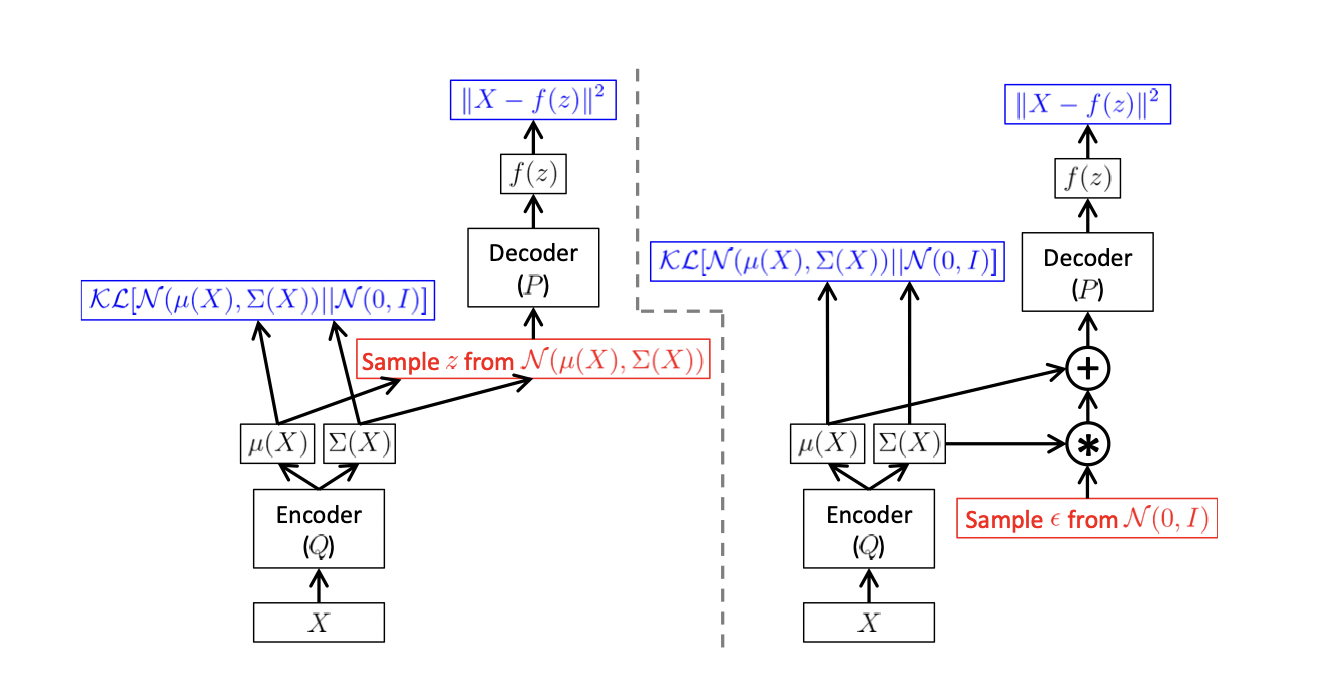
\includegraphics[width=12cm]{images/vae-reparametrisation-trick}
		\blfootnote{Image tirée de \cite{doersch2016tutorial}}
	\end{frame}
	
	\section{Méthode proposée}
	
	\begin{frame}
		\frametitle{Les objectifs}
		\begin{enumerate}
			\item Faire la détection d'anomalies sur des données complexes, par exemple des images.
			\item Avoir un score d'anomalie simple à interpréter et à mettre en pratique, comme un seuil qui s'apparante à un niveau de confiance. 
		\end{enumerate}
	\end{frame}
	
	\begin{frame}
		\frametitle{Les hypothèses}
		\begin{itemize}
			\item Ensemble d'entraînement $\mathcal{X} = \{\boldsymbol{X^{(1)}}, ..., \boldsymbol{X^{(n)}}\}$
				\begin{itemize}
					\item $n$ observations indépendantes de $\boldsymbol{X} \in \mathbb{R}^{d_1 \times d_2}$
					\item $n$ observations proviennent d'un mélange où $(1-p) \in \mathcal{N}$ et $p \not\in \mathcal{N}$
					\item $\mathcal{N}$: population "normale"
					\item on suppose que $p$ est faible (ex: < 5\%)
					\item on ne connait pas la valeur exacte de $p$
				\end{itemize}
			\item Ensemble de test $\mathcal{X^*} = \{\boldsymbol{X^{*(1)}},...,\boldsymbol{X^{*(k)}}\}$
				\begin{itemize}
					\item $k$ observations indépendantes de $\boldsymbol{X^{*}} \in \mathbb{R}^{d_1 \times d_2}$
					\item $k$ observations proviennent d'un mélange où $(1-p^{*}) \in \mathcal{N}$ et $p^{*} \not\in \mathcal{N}$
					\item on suppose que $p^{*}$ est faible et peut être similaire ou différent de $p$
					\item on ne connait pas la valeur exacte de $p^{*}$
				\end{itemize}
		\end{itemize}
	\end{frame}

	\begin{frame}
		\frametitle{Description de l'approche}
		\begin{enumerate}
			\item Entraîner un autoencodeur variationnel.
			\item Définir un cadre décisionnel pour discriminer les observations "normales" des observations "anormales" à partir des représentations latentes et d'un seuil $\alpha$ appelé, \textbf{niveau de filtration}.
		\end{enumerate}
	\end{frame}

	\begin{frame}
		\frametitle{Entraînement du VAE}
		
		Comment orienter l'apprentissage du VAE vers le contenu?
		
		\begin{columns}
			\column{.3\textwidth}
			\centering
			\begin{figure}
				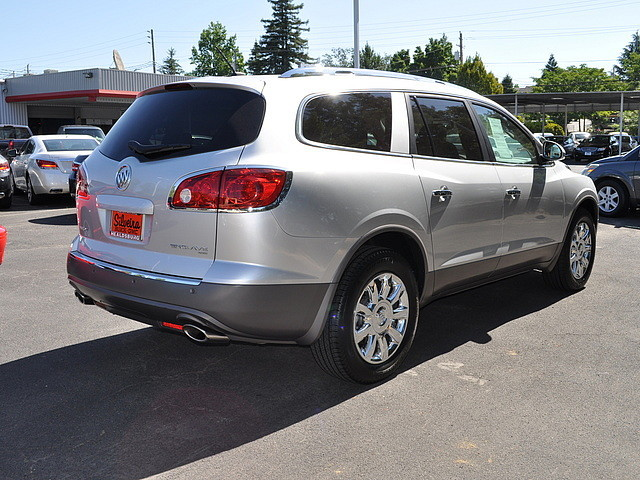
\includegraphics[width=2.5cm,height=1.8cm]{../rapports/images/images_anomalies/inlier-1}
				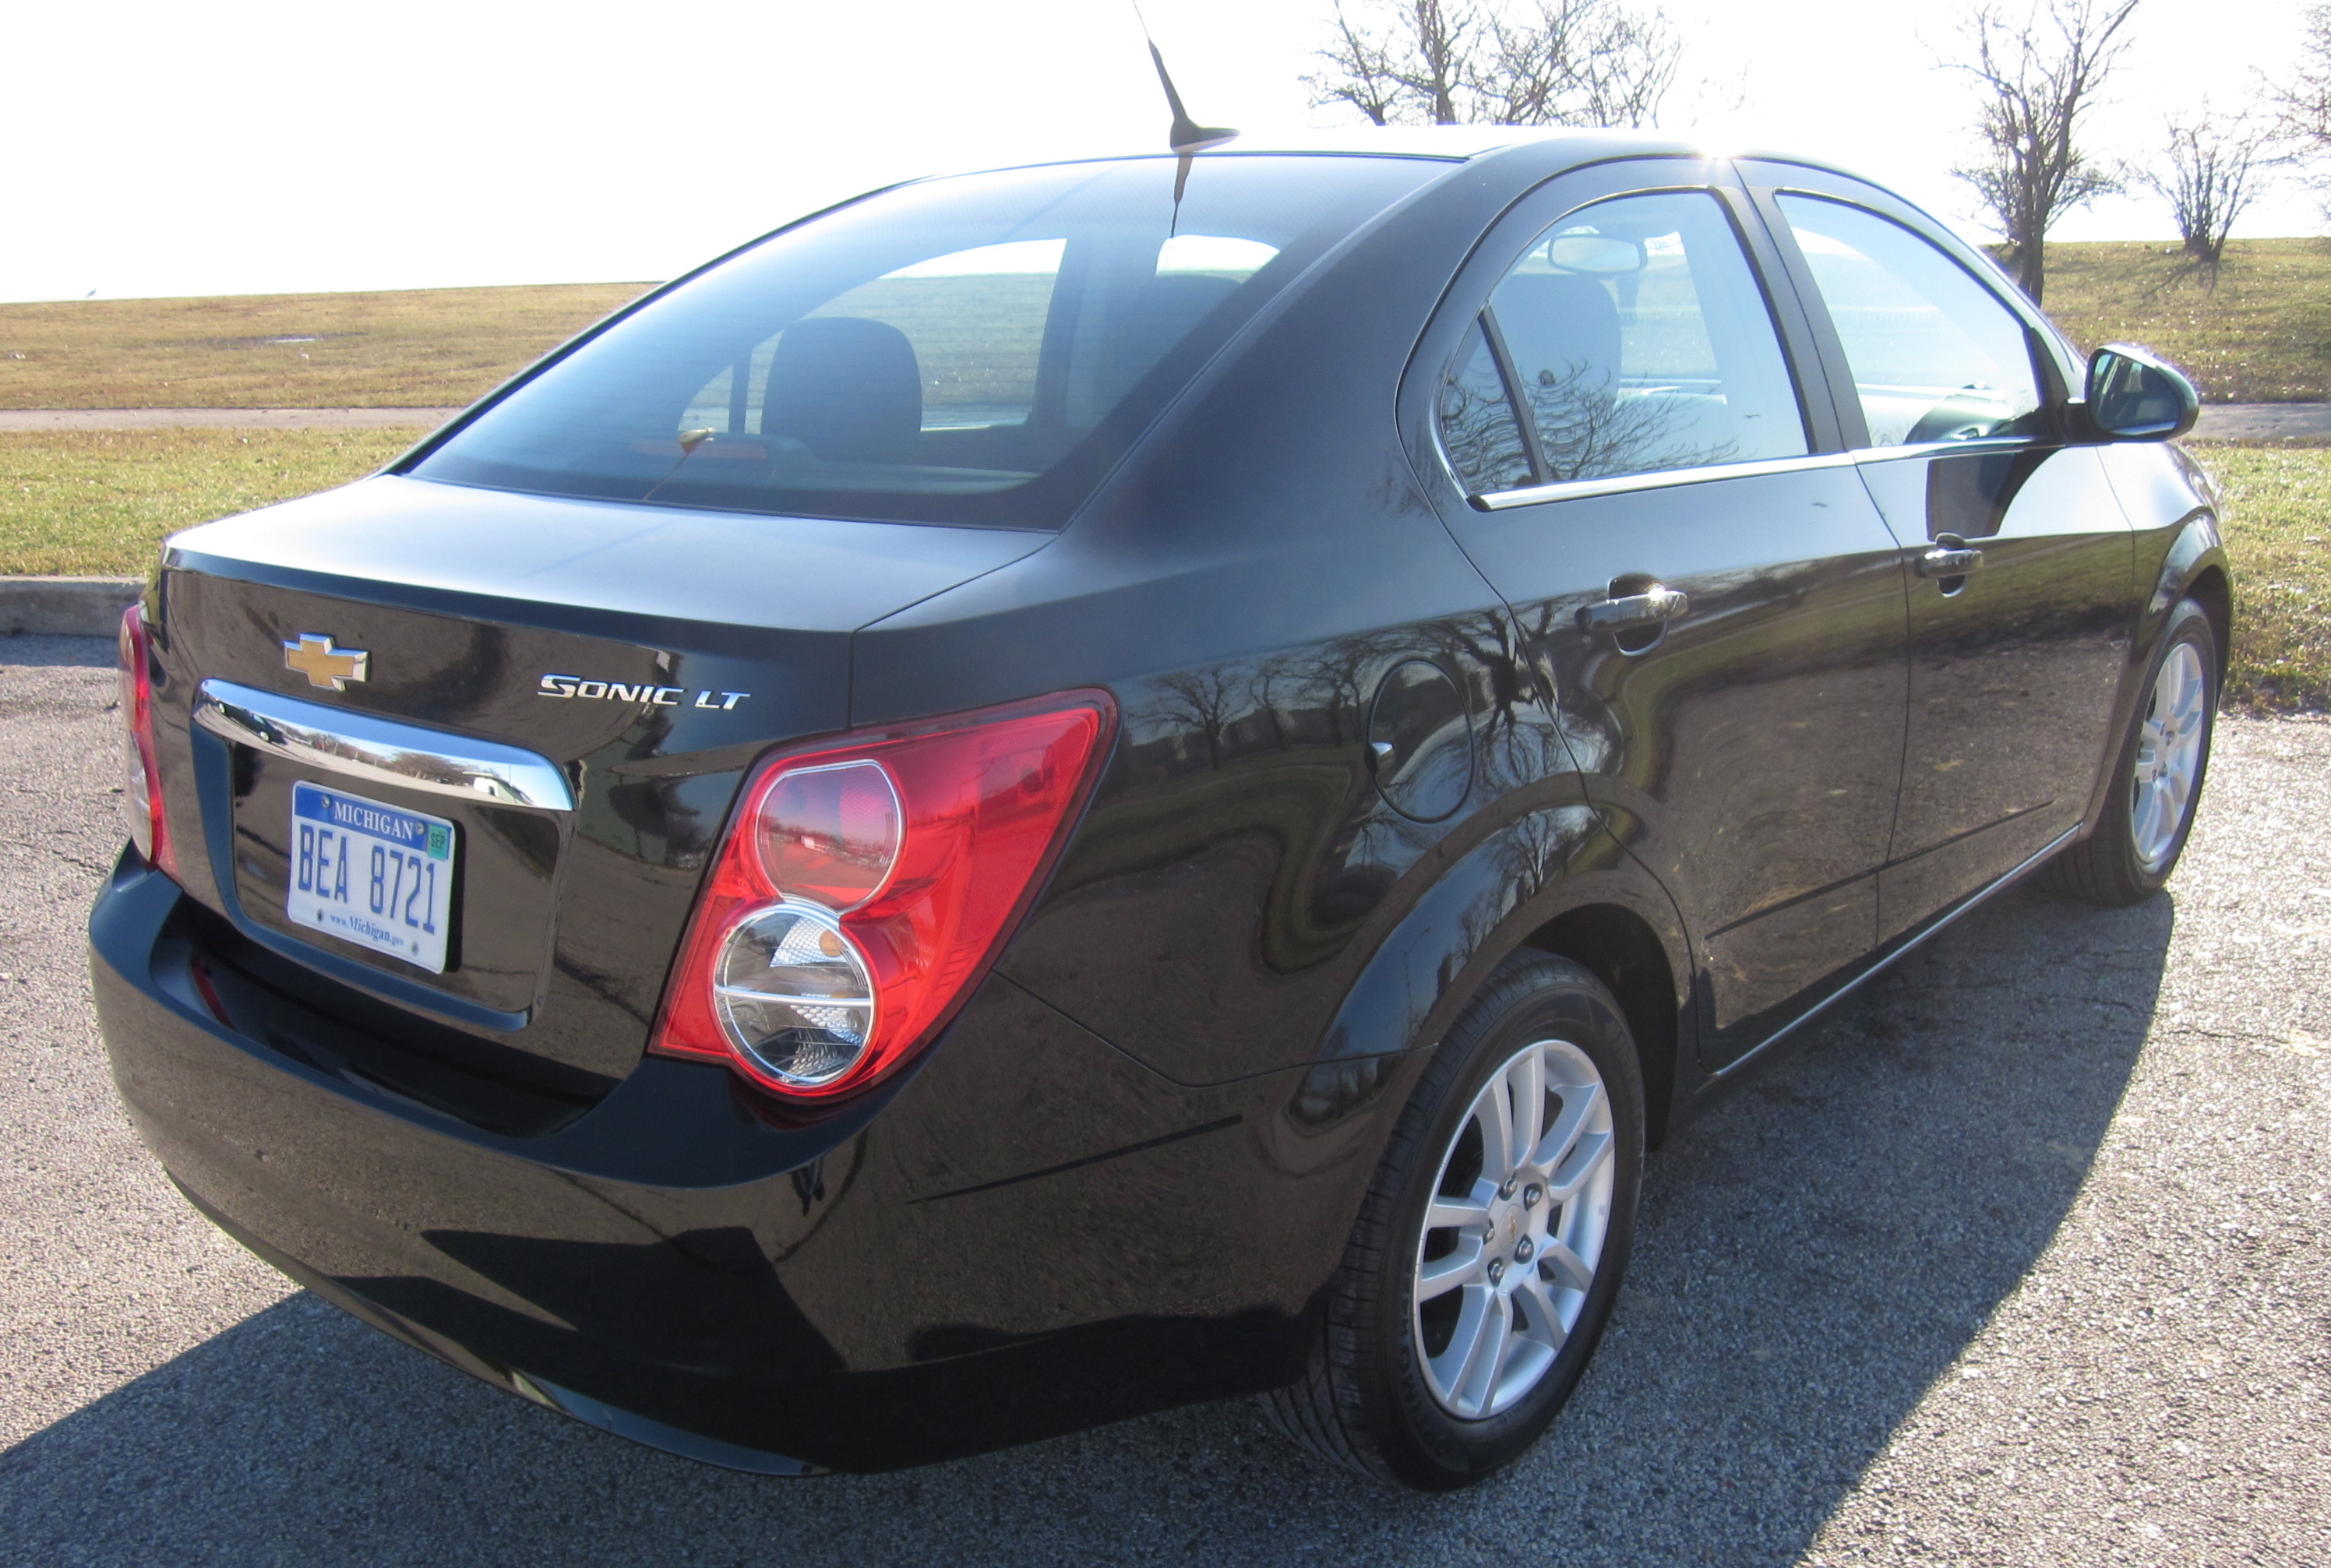
\includegraphics[width=2.5cm,height=1.8cm]{../rapports/images/images_anomalies/inlier-2}
				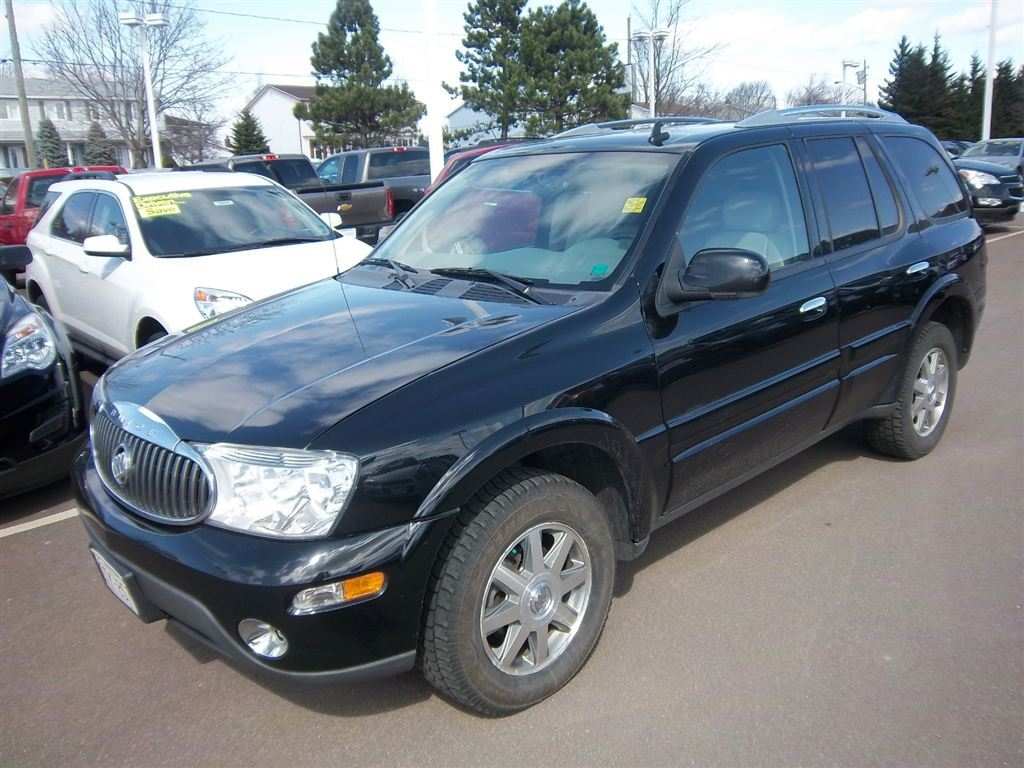
\includegraphics[width=2.5cm,height=1.8cm]{../rapports/images/images_anomalies/inlier-3}
				{\footnotesize Images "normales"}
			\end{figure}
		
			\column{.3\textwidth}
			\centering
			\begin{figure}
			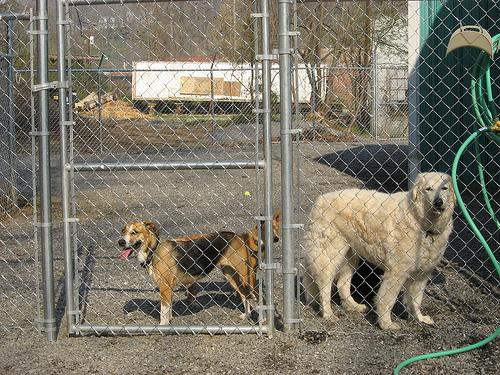
\includegraphics[width=2.5cm,height=1.8cm]{../rapports/images/images_anomalies/anomalie-1}
			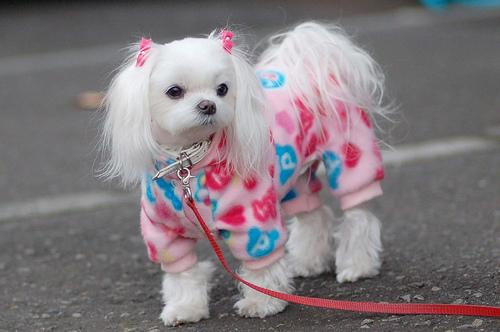
\includegraphics[width=2.5cm,height=1.8cm]{../rapports/images/images_anomalies/anomalie-2}
			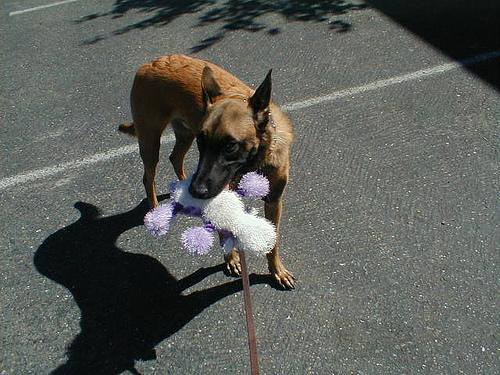
\includegraphics[width=2.5cm,height=1.8cm]{../rapports/images/images_anomalies/anomalie-3}
			{\footnotesize Images "anormales"}
			\end{figure}
		
			\column{.3\textwidth}
			\centering
			\begin{figure}
				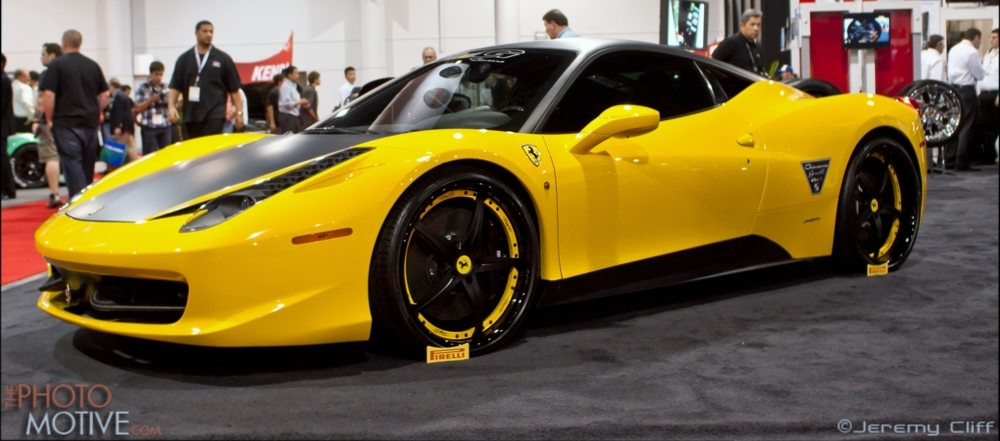
\includegraphics[width=2.5cm,height=1.8cm]{../rapports/images/images_anomalies/inlier-4}
				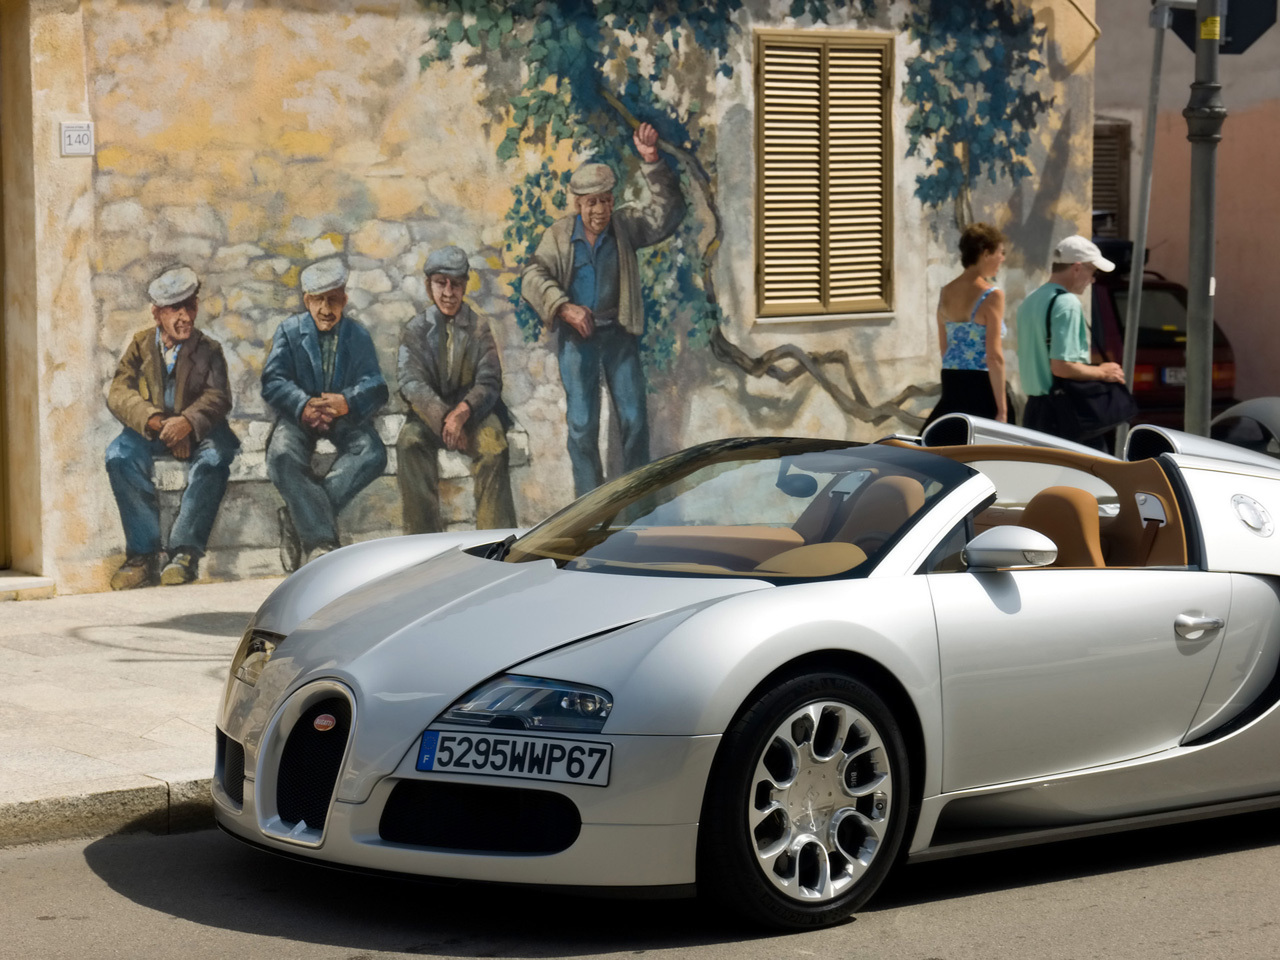
\includegraphics[width=2.5cm,height=1.8cm]{../rapports/images/images_anomalies/inlier-5}
				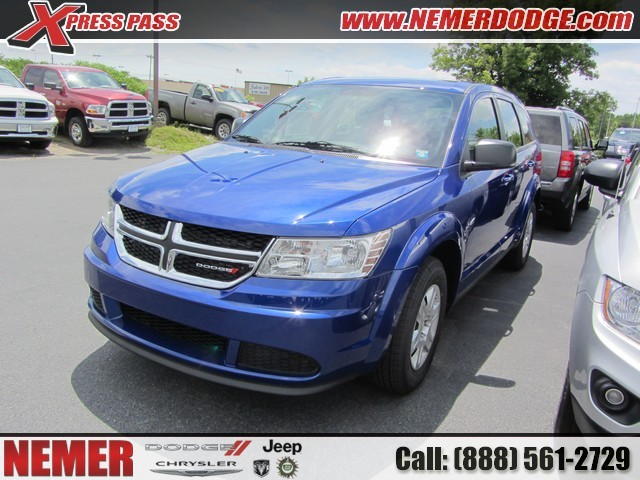
\includegraphics[width=2.5cm,height=1.8cm]{../rapports/images/images_anomalies/inlier-6}
				{\footnotesize Images "normales"}
			\end{figure}
		\end{columns}
	\end{frame}
	
	\begin{frame}
			\frametitle{\textit{Perpceptual loss}}
		
		Pour orienter la perte vers le contenu, on utilise le concept de \textit{perceptual loss} \citep{Johnson2016Perceptual}.
		
		\begin{figure}[h]
			\centering
			\begin{tikzpicture}[shorten >=1pt,draw=black!50, node distance=\layersep, square/.style={regular polygon,regular polygon sides=4}]
				\tikzstyle{neuron}=[circle,fill=black!25,minimum size=30pt,inner sep=0pt]
				\tikzstyle{network}=[square,fill=black!25,minimum size=30pt,inner sep=0pt]
				\tikzstyle{network2}=[rectangle,fill=black!25,minimum size=30pt,inner sep=0pt]
				\tikzstyle{input neuron}=[neuron, fill=green!50];
				\tikzstyle{graph}=[network, fill=white, draw=black];
				\tikzstyle{graph2}=[network2, fill=white, draw=black];
				\tikzstyle{hidden neuron}=[neuron, fill=blue!50];
				\tikzstyle{annot} = [text width=4em, text centered]
				
				% Draw input (x)
				\node[input neuron] (input) at (0,-5) {$\boldsymbol{x}$};
				
				% Draw the VAE 
				\node[graph2] (vae) at (2,-2.5) {  $p_{\phi}(q_{\theta}(\boldsymbol{x}))$ };
				
				% Draw the output (\hat(x)) with x below
				\node[hidden neuron] (x_chap) at (4,-2.5) {$\hat{\boldsymbol{x}}$};
				%\node[input neuron] (input-2) at (6,-5) {$\boldsymbol{x}$};
				
				% Draw the VGG16
				\node[graph] (vgg16_1) at (6,-2.5) {$g(\cdot)$};
				\node[graph] (vgg16_2) at (6,-5) {$g(\cdot)$};
				
				
				% Draw the outputs
				\node[hidden neuron] (input_sortie) at (8,-2.5) {$g(\hat{\boldsymbol{x}})$};
				\node[input neuron] (x_chap_sortie) at (8,-5) {$g(\boldsymbol{x})$};
				
				% Draw arrows
				\path[->, line width=1mm] (input) edge (vae);
				\path[->, line width=1mm] (vae) edge (x_chap);
				\path[->, line width=1mm] (input) edge (vgg16_2);
				\path[->, line width=1mm] (x_chap) edge (vgg16_1);
				\path[->, line width=1mm] (vgg16_1) edge (input_sortie);
				\path[->, line width=1mm] (vgg16_2) edge (x_chap_sortie);
				
				% Annotate the steps
				\node[annot,above of=input, node distance=3.5cm] (h1) {Image d'entrée};
				\node[annot,above of=vae, node distance=1cm] (h2) {VAE};
				\node[annot,above of=vgg16_1, node distance=1cm] (h3) {VGG16*};
			\end{tikzpicture}
			\caption{Mécanisme de la \textit{perceptual loss}}
		\end{figure}
	\end{frame}

	\begin{frame}
		\frametitle{Définir un cadre décisionnel}
		On checher à savoir si les représentations latentes apprises par le VAE nous permettent de discriminer les observations "normales" des observations "anormales.
	\end{frame}

	\begin{frame}
		\frametitle{Définir un cadre décisionnel}
		Le cadre décisionnel se divise en 3 étapes:
		\begin{enumerate}
			\item On encode les représentations latentes vers des statistiques de distance que l'on peut calculer avec une fonction $T(\cdot)$.
			\item On utilise ces statistiques de distance afin d'obtenir un score d'anomalie $\gamma$.
			\item On compare $\gamma$ avec un niveau de filtration $\alpha$ pour savoir si l'observation semble "normale" ou "anormale".
		\end{enumerate}
	\end{frame}

	\begin{frame}
		\frametitle{Définir la statistique de distance}
		Étant donné que nos représentations latentes sont des vecteurs $(\boldsymbol{\mu}, \boldsymbol{\sigma})$, on utilise une distance de Kullback-Leibler pour définir nos statistiques.
		\begin{itemize}
			\item  $T^{(i)} = D_{KL}\big[N(\boldsymbol{\mu^{(i)}}, \boldsymbol{\sigma^{(i)}}) || N(0, I)\big]$
			\item $T_{\mathcal{X}}=\{T^{(1)}, ..., T^{(n)}\}$
		\end{itemize}
		\vfill
		2 scénarios sont possibles:
		\begin{enumerate}
			\item \textbf{Près de la $N(0,I)$:} Les valeurs des statistiques de distance correspondant aux observations "normales" sont faibles
			\item \textbf{Éloigné de la $N(0,I)$:} Les valeurs des statistiques de distance correspondant aux observations "normales" sont élevées
		\end{enumerate}
		
	\end{frame}

	\begin{frame}
		\frametitle{Définir la statistique de distance}
		\begin{figure}
			\centering
			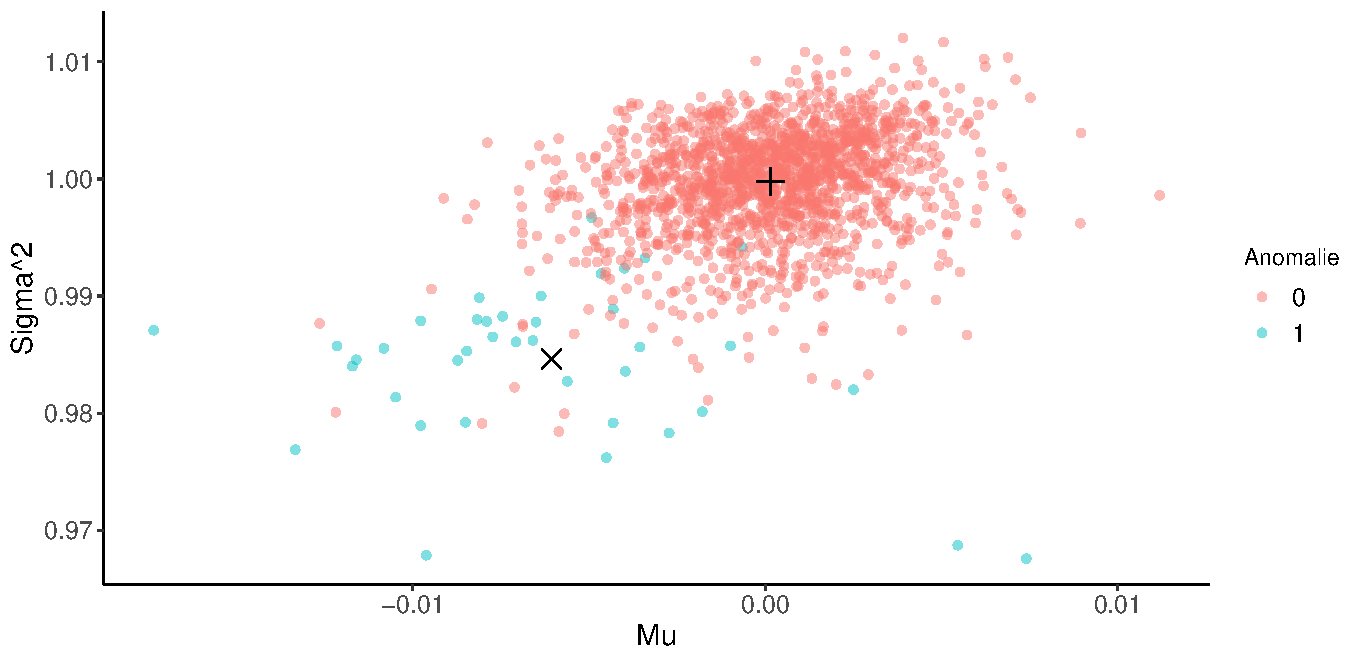
\includegraphics[width=5cm, height=4cm]{../rapports/images/plot_near.pdf}
			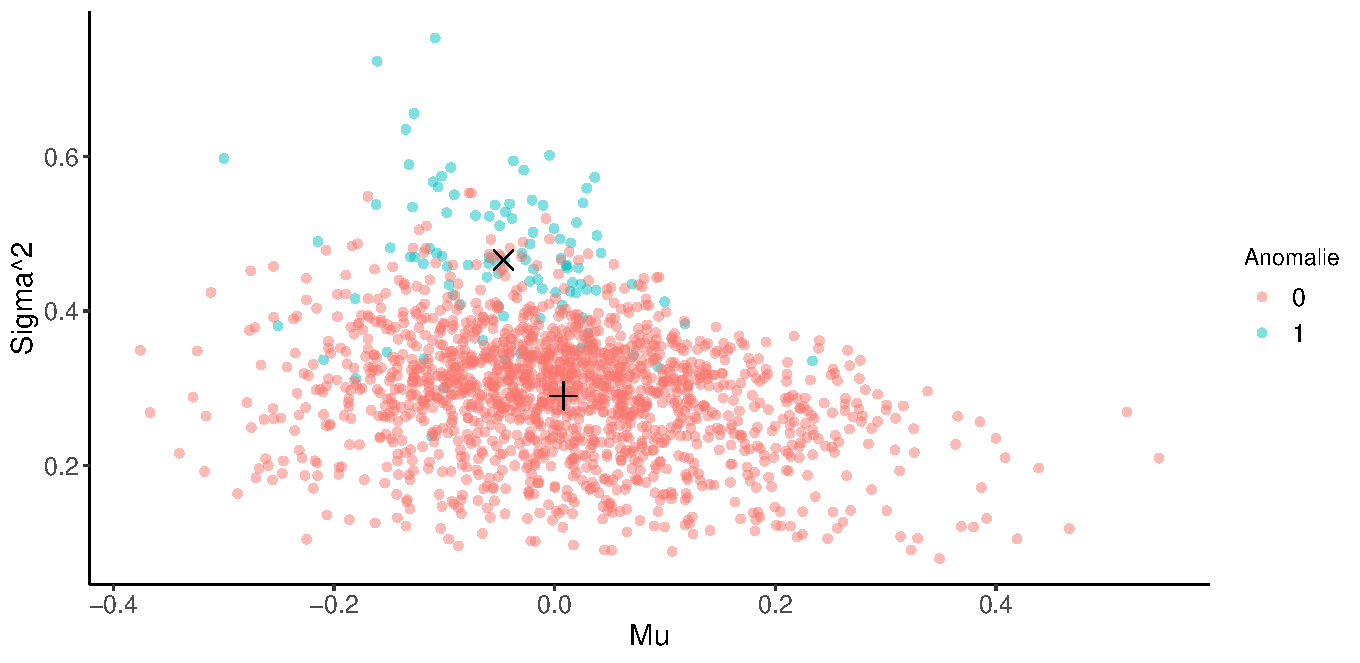
\includegraphics[width=5cm, height=4cm]{../rapports/images/plot_away.pdf}
			\caption{Scénario 1 (gauche) et scénario 2 (droite)}
		\end{figure}
		
	\end{frame}

	\begin{frame}
		\frametitle{Définir le score d'anomalie $\gamma$}
		 Pour trouver le score d'anomalie $\gamma$, on ordonne les statistiques distance selon le scénario et on calcule le rang.
		 \begin{itemize}
		 	\item $T^{'}_{\mathcal{X}}$: l'ensemble $T_{\mathcal{X}}$ ordonné selon le scénario 1 ou 2
		 		\begin{itemize}
		 			\item Scénario 1: $T_{\mathcal{X}}$ en ordre croissant
		 			\item Scénario 2: $T_{\mathcal{X}}$ en ordre décroissant
		 		\end{itemize}
	 		\item $\gamma(\boldsymbol{x^{(j)}}) = \frac{rang_{T^{'}_{\mathcal{X}}}(T^{(j)})}{n}$
	 		\item $rang_{T^{'}_{\mathcal{X}}}(T^{(j)})$ correspond au rang de la statistique de distance $T^{(j)}$ dans l'ensemble ordonné $T^{'}_{\mathcal{X}}$
		 \end{itemize}
		
	\end{frame}

	\begin{frame}
		\frametitle{Résumé de l'approche}
		\begin{center}
			\footnotesize
			\begin{algorithm}[H] \label{alg:metho}
				\SetAlgoLined
				\KwIn{Ensemble de données d'entraînement $\boldsymbol{x^{(i)}}, i=1,...,n$ \\ Ensemble de données de test $\boldsymbol{x^{*(j)}}, j=1, ..., k$}
				\KwOut{Scores d'anomalie $\gamma^{(j)}, j=1,...,k$}
				$\theta$, $\phi$ $\leftarrow$ paramètres de l'encodeur et du  décodeur du VAE entraîné\;
				\For{i=1 to n}{
					$ (\boldsymbol{\mu^{(i)}}, \boldsymbol{\sigma^{(i)}}) = q_{\theta}(\boldsymbol{x^{(i)}})$ \\
					$T_{\mathcal{X}}^{(i)}=D_{KL}\big[N(\boldsymbol{\mu^{(i)}}, \boldsymbol{\sigma^{(i)}}) || N(0, I)\big]$
				}
				Ordonner $T_{\mathcal{X}}$ selon le scénario identifié pour obtenir $T^{'}_{\mathcal{X}}$ \;
				\For{j=1 to k}{
					$(\boldsymbol{\mu^{(j)}}, \boldsymbol{\sigma^{(j)}}) = q_{\theta}(\boldsymbol{x^{*(j)}})$ \\
					$T_{\mathcal{X^*}}^{(j)}=D_{KL}\big[N(\boldsymbol{\mu^{(j)}}, \boldsymbol{\sigma^{(j)}}) || N(0, I)\big]$ \\
					$\gamma(\boldsymbol{x^{*(j)}}) = rang_{T^{'}_{\mathcal{X}}}(T_{\mathcal{X^*}}^{(j)})/n$
				}
				\KwRet{$\gamma^{(j)}, j=1,...,k$}
				\caption{Algorithme de détection d'anomalies}
			\end{algorithm}
		\end{center}
		
	\end{frame}

	\begin{frame}
		\frametitle{Filtrer les anomalies}
		La dernière étape consiste à comparer ces scores avec notre niveau de filtration $\alpha$.
		\begin{itemize}
			\item $\gamma^{(j)} > (1 - \alpha)$: observation $\alpha$-anormale
			\item $\gamma^{(j)} \le (1 - \alpha)$: observation $\alpha$-normale
		\end{itemize}
		
	\end{frame}
	
	\section{Expérimentations}
	
	\subsection{Jeux de données et méthodes testées}
	
	\begin{frame}
		\frametitle{2 jeux de données}
		Voici les 2 jeux de données sur lesquels nous avons testé notre approche:
		\begin{itemize}
			\item MNIST
			\item ImageNet
		\end{itemize}
		
	\end{frame}

	\begin{frame}
		\frametitle{Exemples d'images - MNIST}
		Objectif: Trouver des anomalies dans des chiffres écrits à la main.
		
		\begin{figure}
			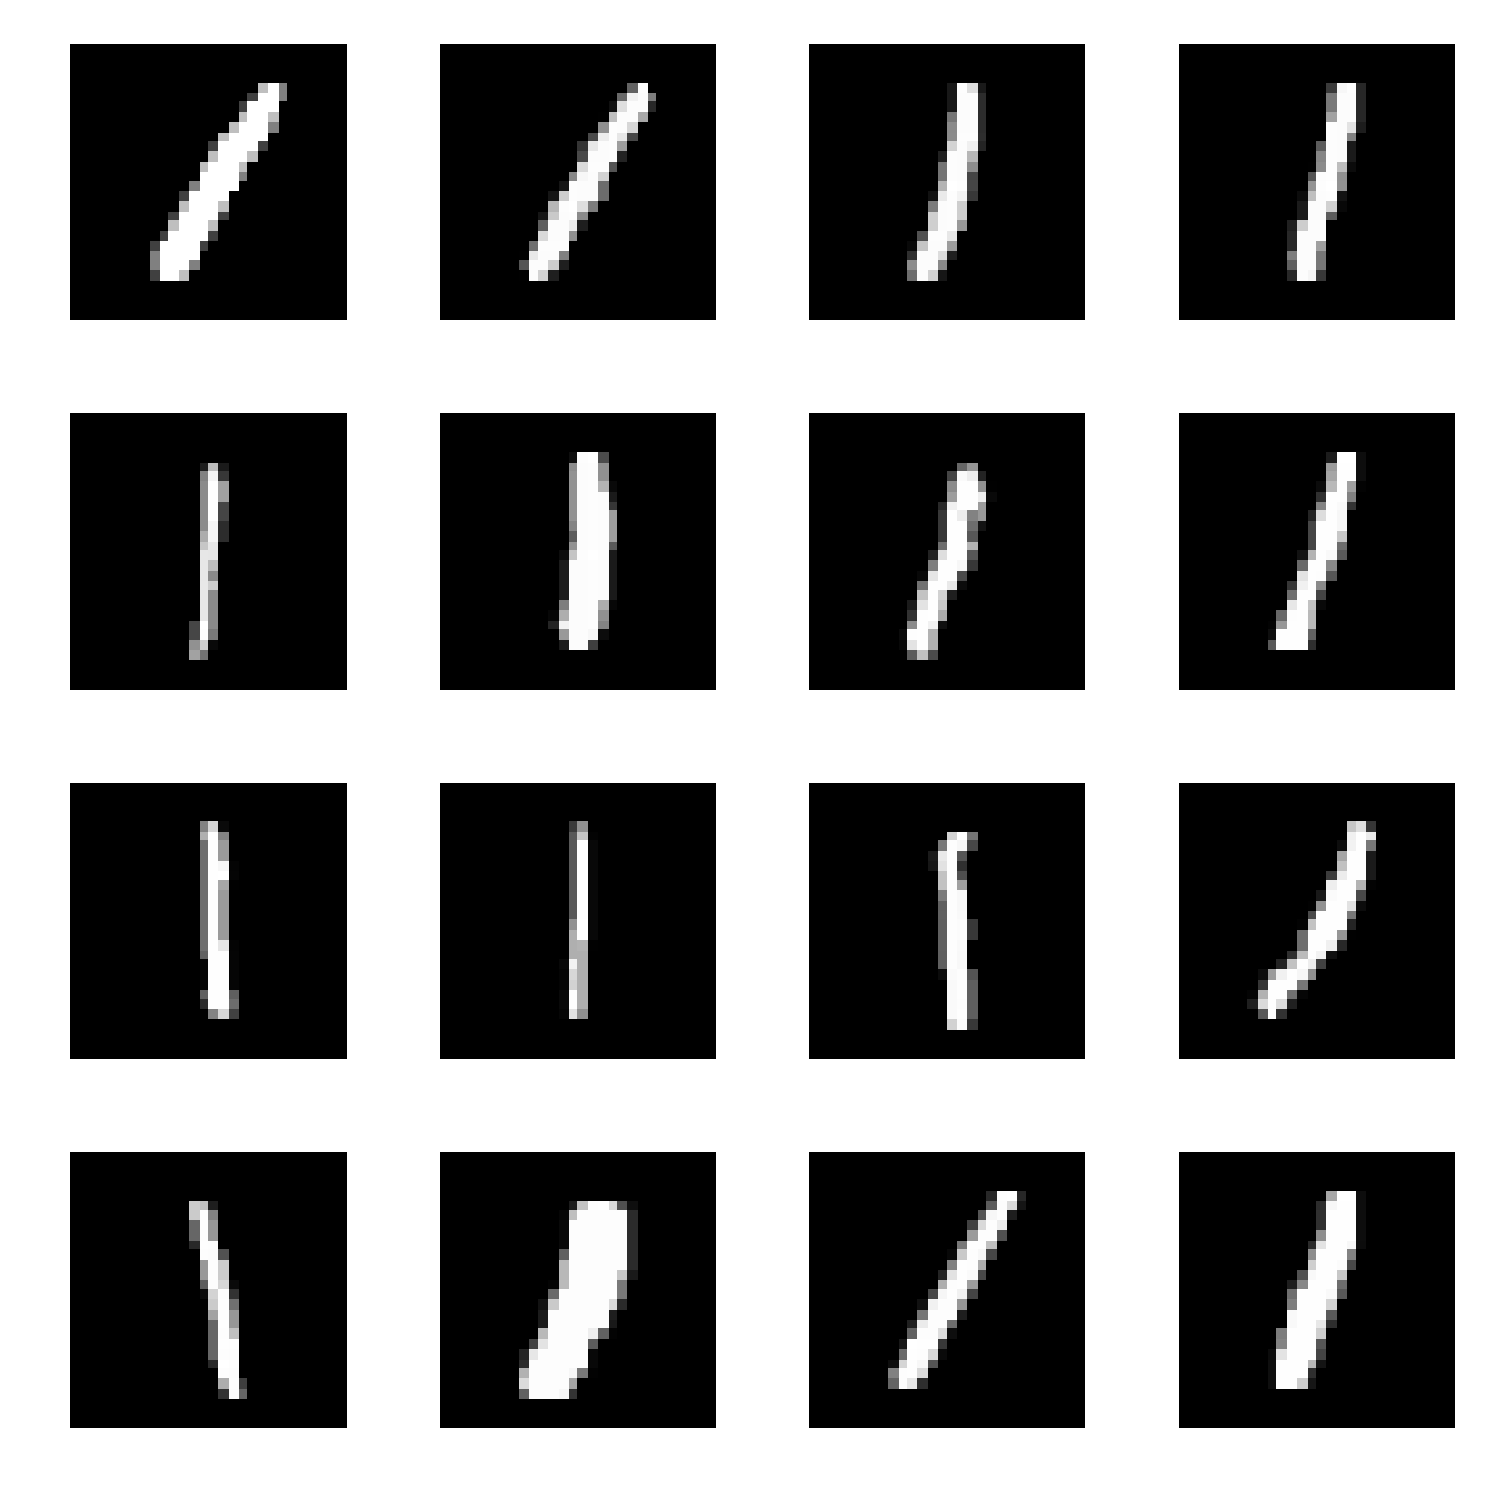
\includegraphics[width=4cm]{../rapports/images/mnist-inliers}
			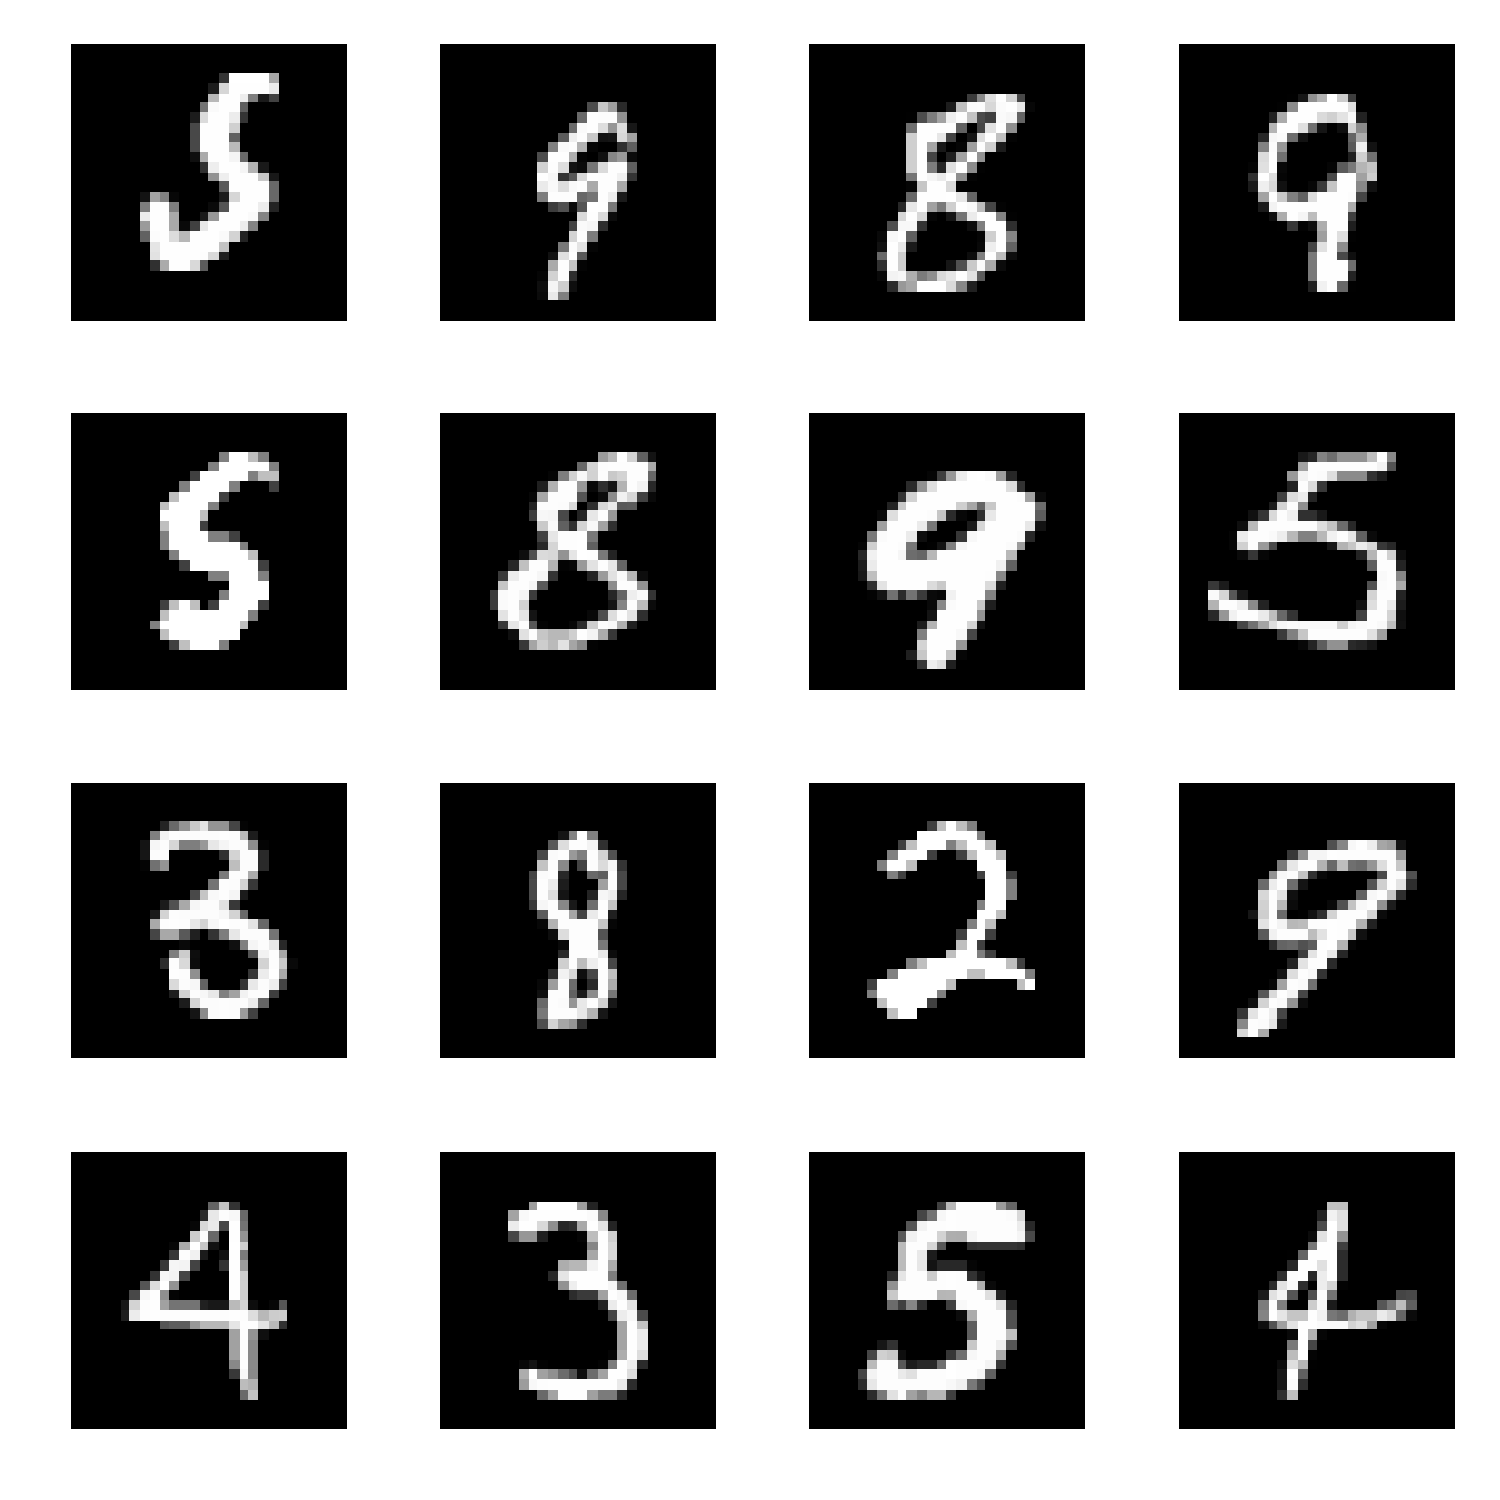
\includegraphics[width=4cm]{../rapports/images/mnist-outliers}
			\caption{La catégorie "normale" (gauche) et la catégorie "anormale" (droite).}
		\end{figure}
		
	\end{frame}


	\begin{frame}
		\frametitle{Exemple d'images - ImageNet}
		Objectif: Trouver des anomalies dans un jeu de données d'images réelles plus complexes.
		
		\begin{figure}
			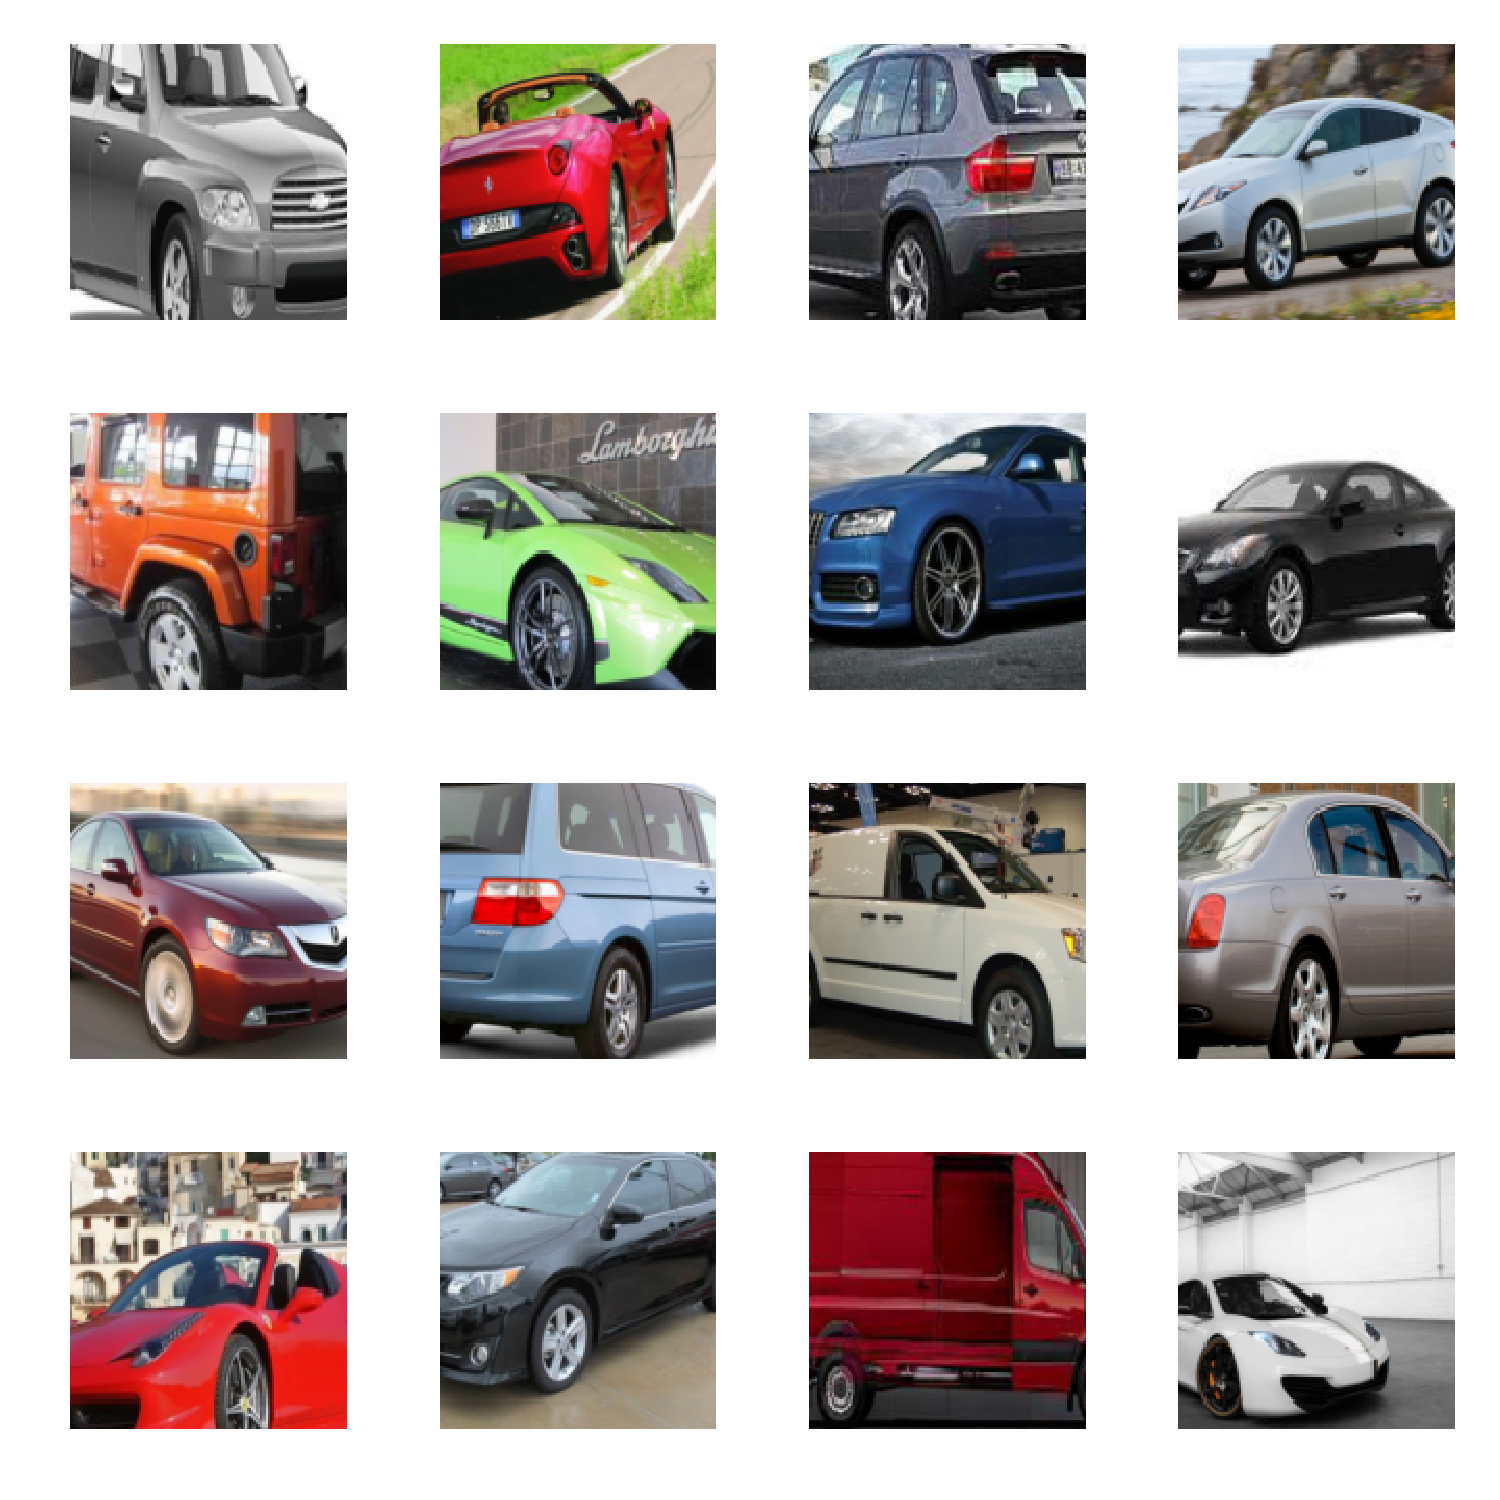
\includegraphics[width=4cm]{../rapports/images/imagenet-inliers}
			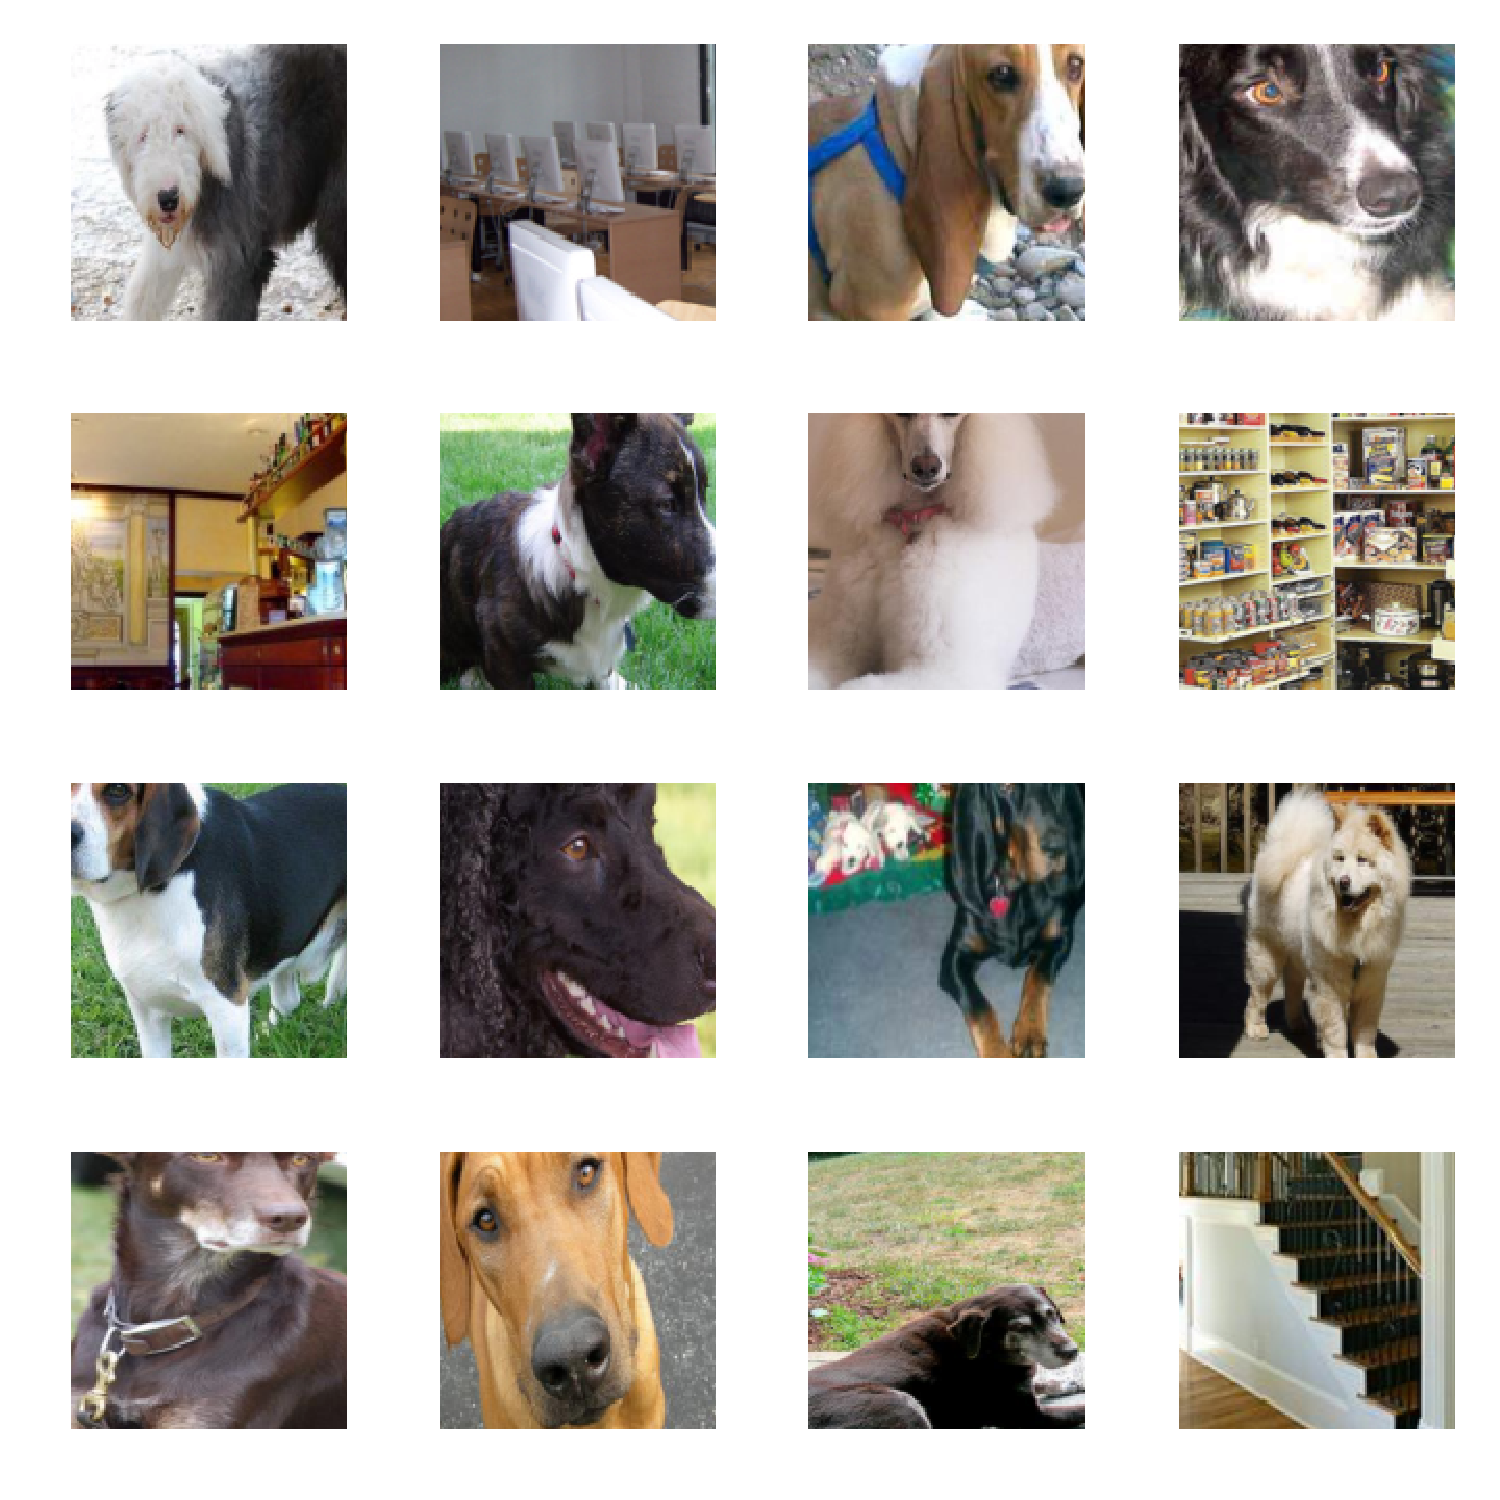
\includegraphics[width=4cm]{../rapports/images/imagenet-outliers}
			\caption{La catégorie "normale" (gauche) et la catégorie "anormale" (droite).}
		\end{figure}
		
	\end{frame}


	\begin{frame}
		\frametitle{Scénarios testés - MNIST}
		
		\resizebox{\textwidth}{!}{%
			\begin{tabular}{| a | a | a |}
				\hline
				\rowcolor{Gray}
				Scénario de test  & Chiffre "normal" & Chiffres "anormaux"  \\
				\hline
				1 & 1 & 5  \\
				2 & 1 & 5,9  \\
				3  & 1 & 0,2,3,4,5,6,7,8,9 \\ 
				4 & 6 & 8  \\
				5 & 6 & 3,8  \\
				6  & 6 & 0,1,2,3,4,5,7,8,9  \\ \hline
			\end{tabular}
		} % end of scope of "\resizebox"  directive		
		
	\end{frame}

	\begin{frame}
		\frametitle{Différents niveaux de contamination - MNIST}
		
		\resizebox{\textwidth}{!}{%
			\begin{tabular}{| c | c | c | c |}
				\hline
				\rowcolor{Gray}
				Contamination & Ensemble de données  & Nombre d'instances & Pourcentage d'anomalies  \\
				\hline
				\multirow{2}{*}{Moins} 
				& $\mathcal{X}$ & 4000 & 10\%  \\
				& $\mathcal{X^*}$  & 800 & 1\%  \\ 
				\midrule
				\multirow{2}{*}{Égal} 
				& $\mathcal{X}$ & 4000 & 5\%  \\
				& $\mathcal{X^*}$  & 800 & 5\%  \\ 
				\midrule
				\multirow{2}{*}{Plus} 
				& $\mathcal{X}$ & 4000 & 1\%  \\
				& $\mathcal{X^*}$  & 800 & 10\%  \\ 
				\midrule
			\end{tabular}
		} % end of scope of "\resizebox"  directive
		
	\end{frame}

	\begin{frame}
		\frametitle{Différents niveaux de contamination - ImageNet}
		
		\resizebox{\textwidth}{!}{%
			\begin{tabular}{| c | c | c | c |}
				\hline
				\rowcolor{Gray}
				Contamination & Ensemble de données  & Nombre d'instances & Pourcentage d'anomalies  \\
				\hline
				\multirow{2}{*}{Moins} 
				& $\mathcal{X}$ & 10000 & 10\%  \\
				& $\mathcal{X^*}$  & 1000 & 1\%  \\ 
				\midrule
				\multirow{2}{*}{Égal} 
				& $\mathcal{X}$ & 10000 & 5\%  \\
				& $\mathcal{X^*}$  & 1000 & 5\%  \\ 
				\midrule
				\multirow{2}{*}{Plus} 
				& $\mathcal{X}$ & 10000 & 1\%  \\
				& $\mathcal{X^*}$  & 1000 & 10\%  \\ 
				\midrule
			\end{tabular}
		} % end of scope of "\resizebox"  directive
		
	\end{frame}

		\begin{frame}
		\frametitle{Méthodes testées}
		Nous avons testé différentes méthodes sur ces scénarios de test:
		\begin{itemize}
			\item PCA: analyse en composantes principales
			\item AE: autoencodeur traditionnel
			\item ISOF-VAE: Isolation Forest appliqué sur la représentation latente du VAE
			\item DA-VAE: méthode que nous proposons
		\end{itemize}
	
		Plus d'informations sur les autres méthodes, voir \hyperlink{supplemental}{\beamerbutton{l'appendice}}.
		
	\end{frame}

	\begin{frame}
		\frametitle{Détails sur DA-VAE - MNIST}
		
		\centering
		
		\begin{tikzpicture}[shorten >=1pt,draw=black!50, node distance=\layersep, square/.style={regular polygon,regular polygon sides=4}, scale=0.6]
			\tikzstyle{box}=[square,fill=white,minimum size=2cm,inner sep=-19pt, draw=black, text width=2cm, text centered, scale=0.6]
			\tikzstyle{annot} = [text width=4em, text centered, scale =0.6]
			
			% Draw different layers
			\node[box,fill=yellow!50] (input) at (0,0) {\tiny Entrée \\ $1 \PLH 28 \PLH 28$};
			\node[box,fill=green!50] (conv1) at (2,0) {\tiny Conv-2D + \\ Max-pooling $16 \PLH 14 \PLH 14$};
			\node[box,fill=green!50] (conv2) at (4,0) {\tiny Conv-2D + \\ Max-pooling $32 \PLH 7 \PLH 7$};
			\node[box,fill=green!50] (conv3) at (6,0) {\tiny 0-padding \\ $32 \PLH 8 \PLH 8$};
			\node[box,fill=green!50] (conv4) at (8,0) {\tiny Conv-2D + \\ Max-pooling $64 \PLH 4 \PLH 4$};
			\node[box,fill=yellow!50] (flatten) at (10,0) {\tiny Flatten \\ $1 \PLH 1024$};
			\node[box,fill=black!30] (mu) at (12,1.2) {\tiny Linéaire \\ $1 \PLH 25$};
			\node[box,fill=black!30] (sigma) at (12,-1.2) {\tiny Linéaire \\ $1 \PLH 25$};
			\node[box,fill=yellow!50] (z) at (14,0) {\tiny $z$ \\ $1 \PLH 25$};
			
			% Draw arrows
			\path[->, line width=1mm] (input) edge (conv1);
			\path[->, line width=1mm] (conv1) edge (conv2);
			\path[->, line width=1mm] (conv2) edge (conv3);
			\path[->, line width=1mm] (conv3) edge (conv4);
			\path[->, line width=1mm] (conv4) edge (flatten);
			\path[->, line width=1mm] (flatten) edge (mu);
			\path[->, line width=1mm] (flatten) edge (sigma);
			\path[->, line width=1mm] (mu) edge (z);
			\path[->, line width=1mm] (sigma) edge (z);
			
			\node[annot,above of=mu, node distance=1cm] (h2) {$\mu$};
			\node[annot,above of=sigma, node distance=1cm] (h3) {$\sigma$};
			
		\end{tikzpicture}
	
		\vspace{1cm}
		
		\begin{tikzpicture}[shorten >=1pt,draw=black!50, node distance=\layersep, square/.style={regular polygon,regular polygon sides=4}, scale=0.6]
			\tikzstyle{box}=[square,fill=white,minimum size=2cm,inner sep=-20pt, draw=black, text width=2cm, text centered, scale=0.6]
			\tikzstyle{annot} = [text width=4em, text centered, scale=0.6]
			
			% Draw different layers
			\node[box,fill=yellow!50] (z) at (0,0) {\tiny $z$ \\ $1 \PLH 25$};
			\node[box,fill=black!30] (linear3) at (2,0) {\tiny Linéaire \\ $1 \PLH 1024$};
			\node[box,fill=yellow!50] (unflatten) at (4,0) {\tiny Unflatten \\ $64 \PLH 4 \PLH 4$};
			\node[box,fill=green!50] (deconv1) at (6,0) {\tiny Deconv-2D \\ $64 \PLH 8 \PLH 8$};
			\node[box,fill=green!50] (deconv2) at (8,0) {\tiny Deconv-2D \\ $32 \PLH 16 \PLH 16$};
			\node[box,fill=green!50] (deconv3) at (10,0) {\tiny Deconv-2D \\ $16 \PLH 28 \PLH 28$};
			\node[box,fill=green!50] (deconv4) at (12,0) {\tiny Conv-2D \\ $1 \PLH 28 \PLH 28$};
			\node[box,fill=yellow!50] (output) at (14,0) {\tiny Sortie \\ $1 \PLH 28 \PLH 28$};
			
			% Draw arrows
			\path[->, line width=1mm] (z) edge (linear3);
			\path[->, line width=1mm] (linear3) edge (unflatten);
			\path[->, line width=1mm] (unflatten) edge (deconv1);
			\path[->, line width=1mm] (deconv1) edge (deconv2);
			\path[->, line width=1mm] (deconv2) edge (deconv3);
			\path[->, line width=1mm] (deconv3) edge (deconv4);
			\path[->, line width=1mm] (deconv4) edge (output);
			
		\end{tikzpicture}
		
	\end{frame}

	\begin{frame}
		\frametitle{Détails sur DA-VAE - ImageNet}
		
		\centering
				\begin{tikzpicture}[shorten >=1pt,draw=black!50, node distance=\layersep, square/.style={regular polygon,regular polygon sides=4}, scale=0.6]
					\tikzstyle{box}=[square,fill=white,minimum size=2cm,inner sep=-20pt, draw=black, text width=2cm, text centered, scale=0.6]
					\tikzstyle{annot} = [text width=4em, text centered, scale=0.6]
					
					% Draw different layers
					\node[box,fill=yellow!50] (input) at (0,0) {\tiny Entrée \\ $3 \PLH 128 \PLH 128$};
					\node[box,fill=green!50] (conv1) at (2,0) {\tiny Conv-2D $16 \PLH 128 \PLH 128$};
					\node[box,fill=green!50] (conv2) at (4,0) {\tiny Conv-2D $128 \PLH 64 \PLH 64$};
					\node[box,fill=green!50] (conv3) at (6,0) {\tiny Conv-2D $256 \PLH 32 \PLH 32$};
					\node[box,fill=green!50] (conv4) at (8,0) {\tiny Conv-2D $512 \PLH 16 \PLH 16$};
					\node[box,fill=yellow!50] (flatten) at (10,0) {\tiny Flatten \\ $1 \PLH 131 072$};
					\node[box,fill=black!30] (mu) at (12,1.2) {\tiny Linéaire \\ $1 \PLH 25$};
					\node[box,fill=black!30] (sigma) at (12,-1.2) {\tiny Linéaire \\ $1 \PLH 25$};
					\node[box,fill=yellow!50] (z) at (14,0) {\tiny $z$ \\ $1 \PLH 25$};
					
					% Draw arrows
					\path[->, line width=1mm] (input) edge (conv1);
					\path[->, line width=1mm] (conv1) edge (conv2);
					\path[->, line width=1mm] (conv2) edge (conv3);
					\path[->, line width=1mm] (conv3) edge (conv4);
					\path[->, line width=1mm] (conv4) edge (flatten);
					\path[->, line width=1mm] (flatten) edge (mu);
					\path[->, line width=1mm] (flatten) edge (sigma);
					\path[->, line width=1mm] (mu) edge (z);
					\path[->, line width=1mm] (sigma) edge (z);
					
					\node[annot,above of=mu, node distance=1cm] (h2) {$\mu$};
					\node[annot,above of=sigma, node distance=1cm] (h3) {$\sigma$};
					
				\end{tikzpicture}
			
				\vspace{1cm}
				
				\begin{tikzpicture}[shorten >=1pt,draw=black!50, node distance=\layersep, square/.style={regular polygon,regular polygon sides=4}, scale=0.6]
					\tikzstyle{box}=[square,fill=white,minimum size=2cm,inner sep=-20pt, draw=black, text width=2cm, text centered, scale=0.6]
					\tikzstyle{annot} = [text width=4em, text centered, scale=0.6]
					
					% Draw different layers
					\node[box,fill=yellow!50] (z) at (0,0) {\tiny $z$ \\ $1 \PLH 25$};
					\node[box,fill=black!30] (linear3) at (2,0) {\tiny Linéaire \\ $1 \PLH 131 072$};
					\node[box,fill=yellow!50] (unflatten) at (4,0) {\tiny Unflatten \\ $512 \PLH 16 \PLH 16$};
					\node[box,fill=green!50] (deconv1) at (6,0) {\tiny Deconv-2D $256 \PLH 32 \PLH 32$};
					\node[box,fill=green!50] (deconv2) at (8,0) {\tiny Deconv-2D $128 \PLH 64 \PLH 64$};
					\node[box,fill=green!50] (deconv3) at (10,0) {\tiny Deconv-2D $16 \PLH 128 \PLH 128$};
					\node[box,fill=green!50] (deconv4) at (12,0) {\tiny Deconv-2D $3 \PLH 128 \PLH 128$};
					\node[box,fill=yellow!50] (output) at (14,0) {\tiny Sortie \\ $3 \PLH 128 \PLH 128$};
					
					% Draw arrows
					\path[->, line width=1mm] (z) edge (linear3);
					\path[->, line width=1mm] (linear3) edge (unflatten);
					\path[->, line width=1mm] (unflatten) edge (deconv1);
					\path[->, line width=1mm] (deconv1) edge (deconv2);
					\path[->, line width=1mm] (deconv2) edge (deconv3);
					\path[->, line width=1mm] (deconv3) edge (deconv4);
					\path[->, line width=1mm] (deconv4) edge (output);
					
				\end{tikzpicture}
		
	\end{frame}
	
	\subsection{Résultats}
	
	\begin{frame}
		\frametitle{Résultats -  MNIST}
		
		Résultats en aire sous la courbe ROC (AUC).
		
		\vspace{0.5cm}
		
		\centering
		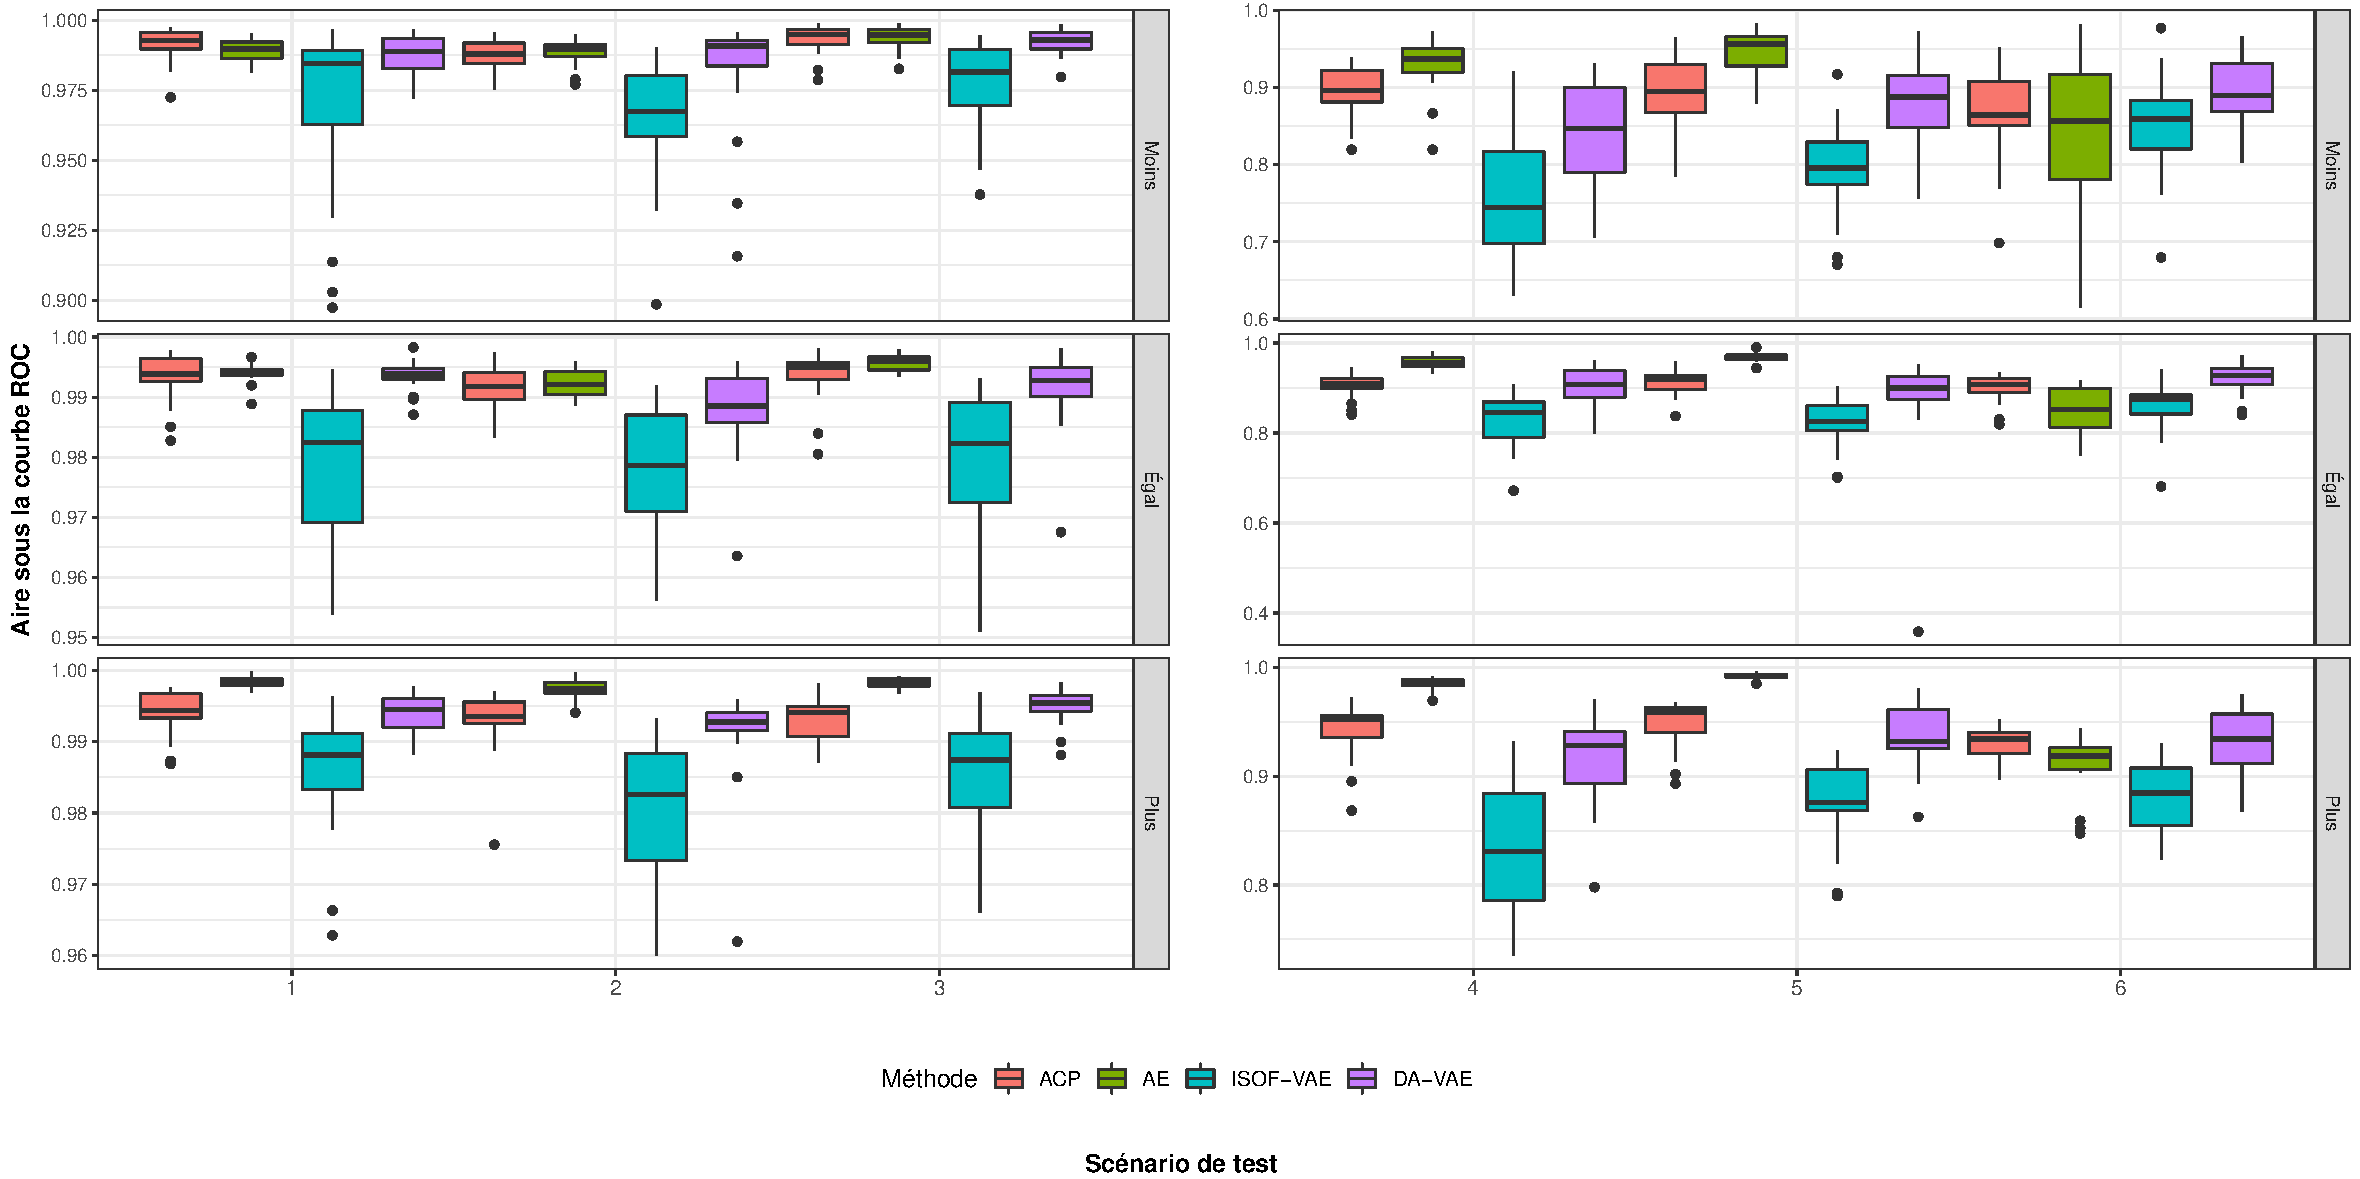
\includegraphics[width=10cm]{../rapports/images/images_boxplots/auc_mnist.pdf}
		
	\end{frame}

	\begin{frame}
		\frametitle{Résultats -  MNIST}
		
		Résultats sur les anomalies (jaunes) et les observations "normales" (mauves) du jeu de données $\mathcal{X^*}$.
		
		\vspace{0.5cm}
		
		\centering
		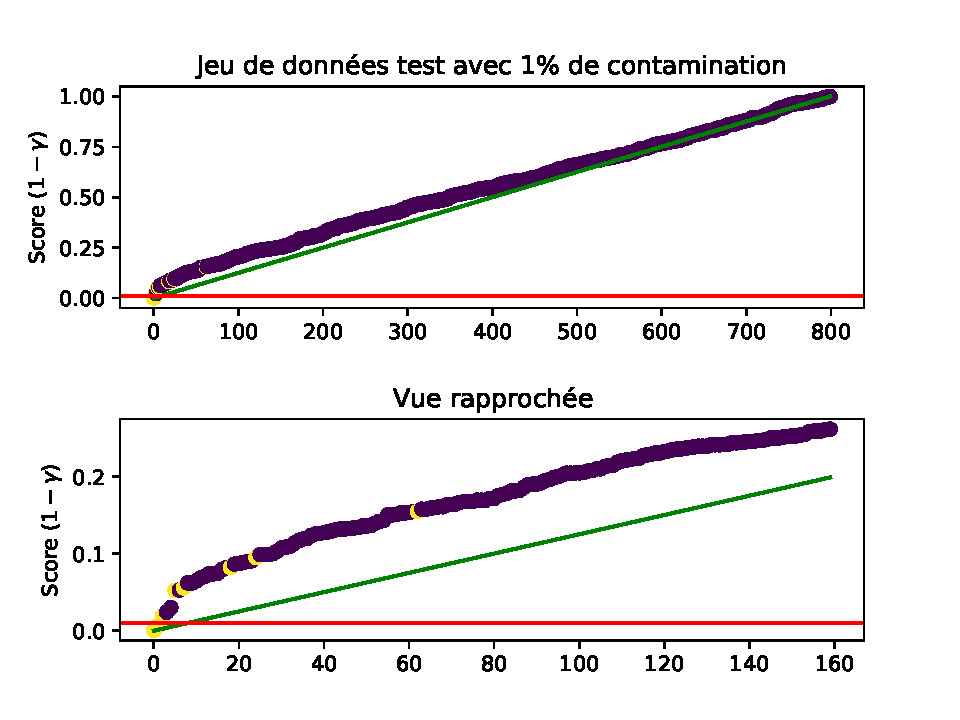
\includegraphics[width=4cm]{../rapports/images/images_davae/pvalues_scenario3_moins}
		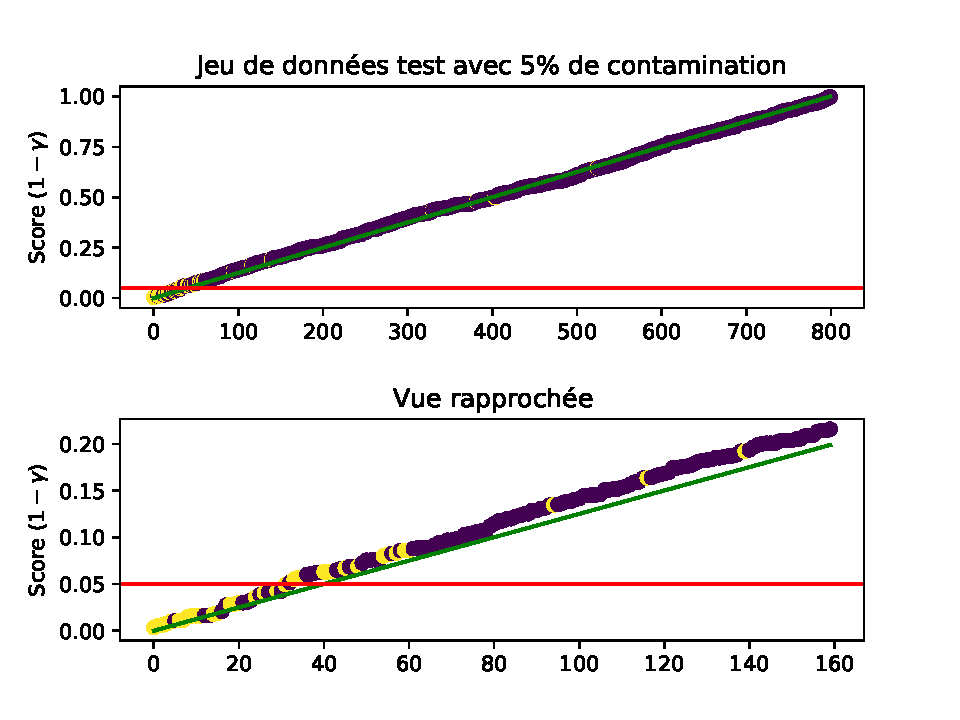
\includegraphics[width=4cm]{../rapports/images/images_davae/pvalues_scenario3_egal}
		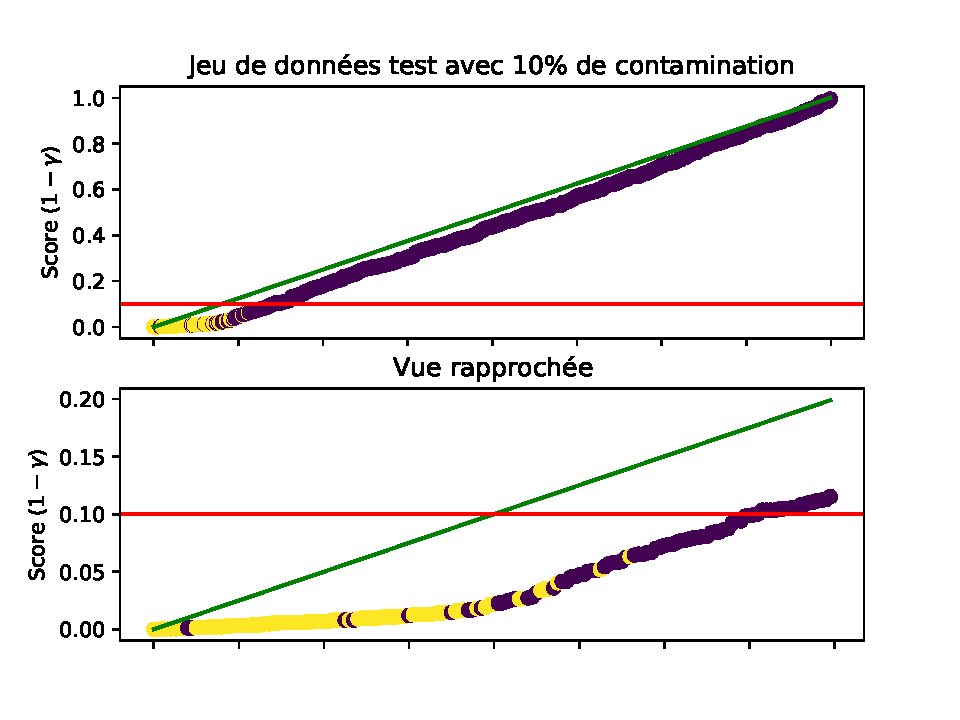
\includegraphics[width=4cm]{../rapports/images/images_davae/pvalues_scenario3_plus}
		
	\end{frame}
	
	\begin{frame}
		\frametitle{Résultats -  ImageNet}
		
		Résultats en aire sous la courbe ROC (AUC).
		
		\vspace{0.5cm}
		
		\centering
		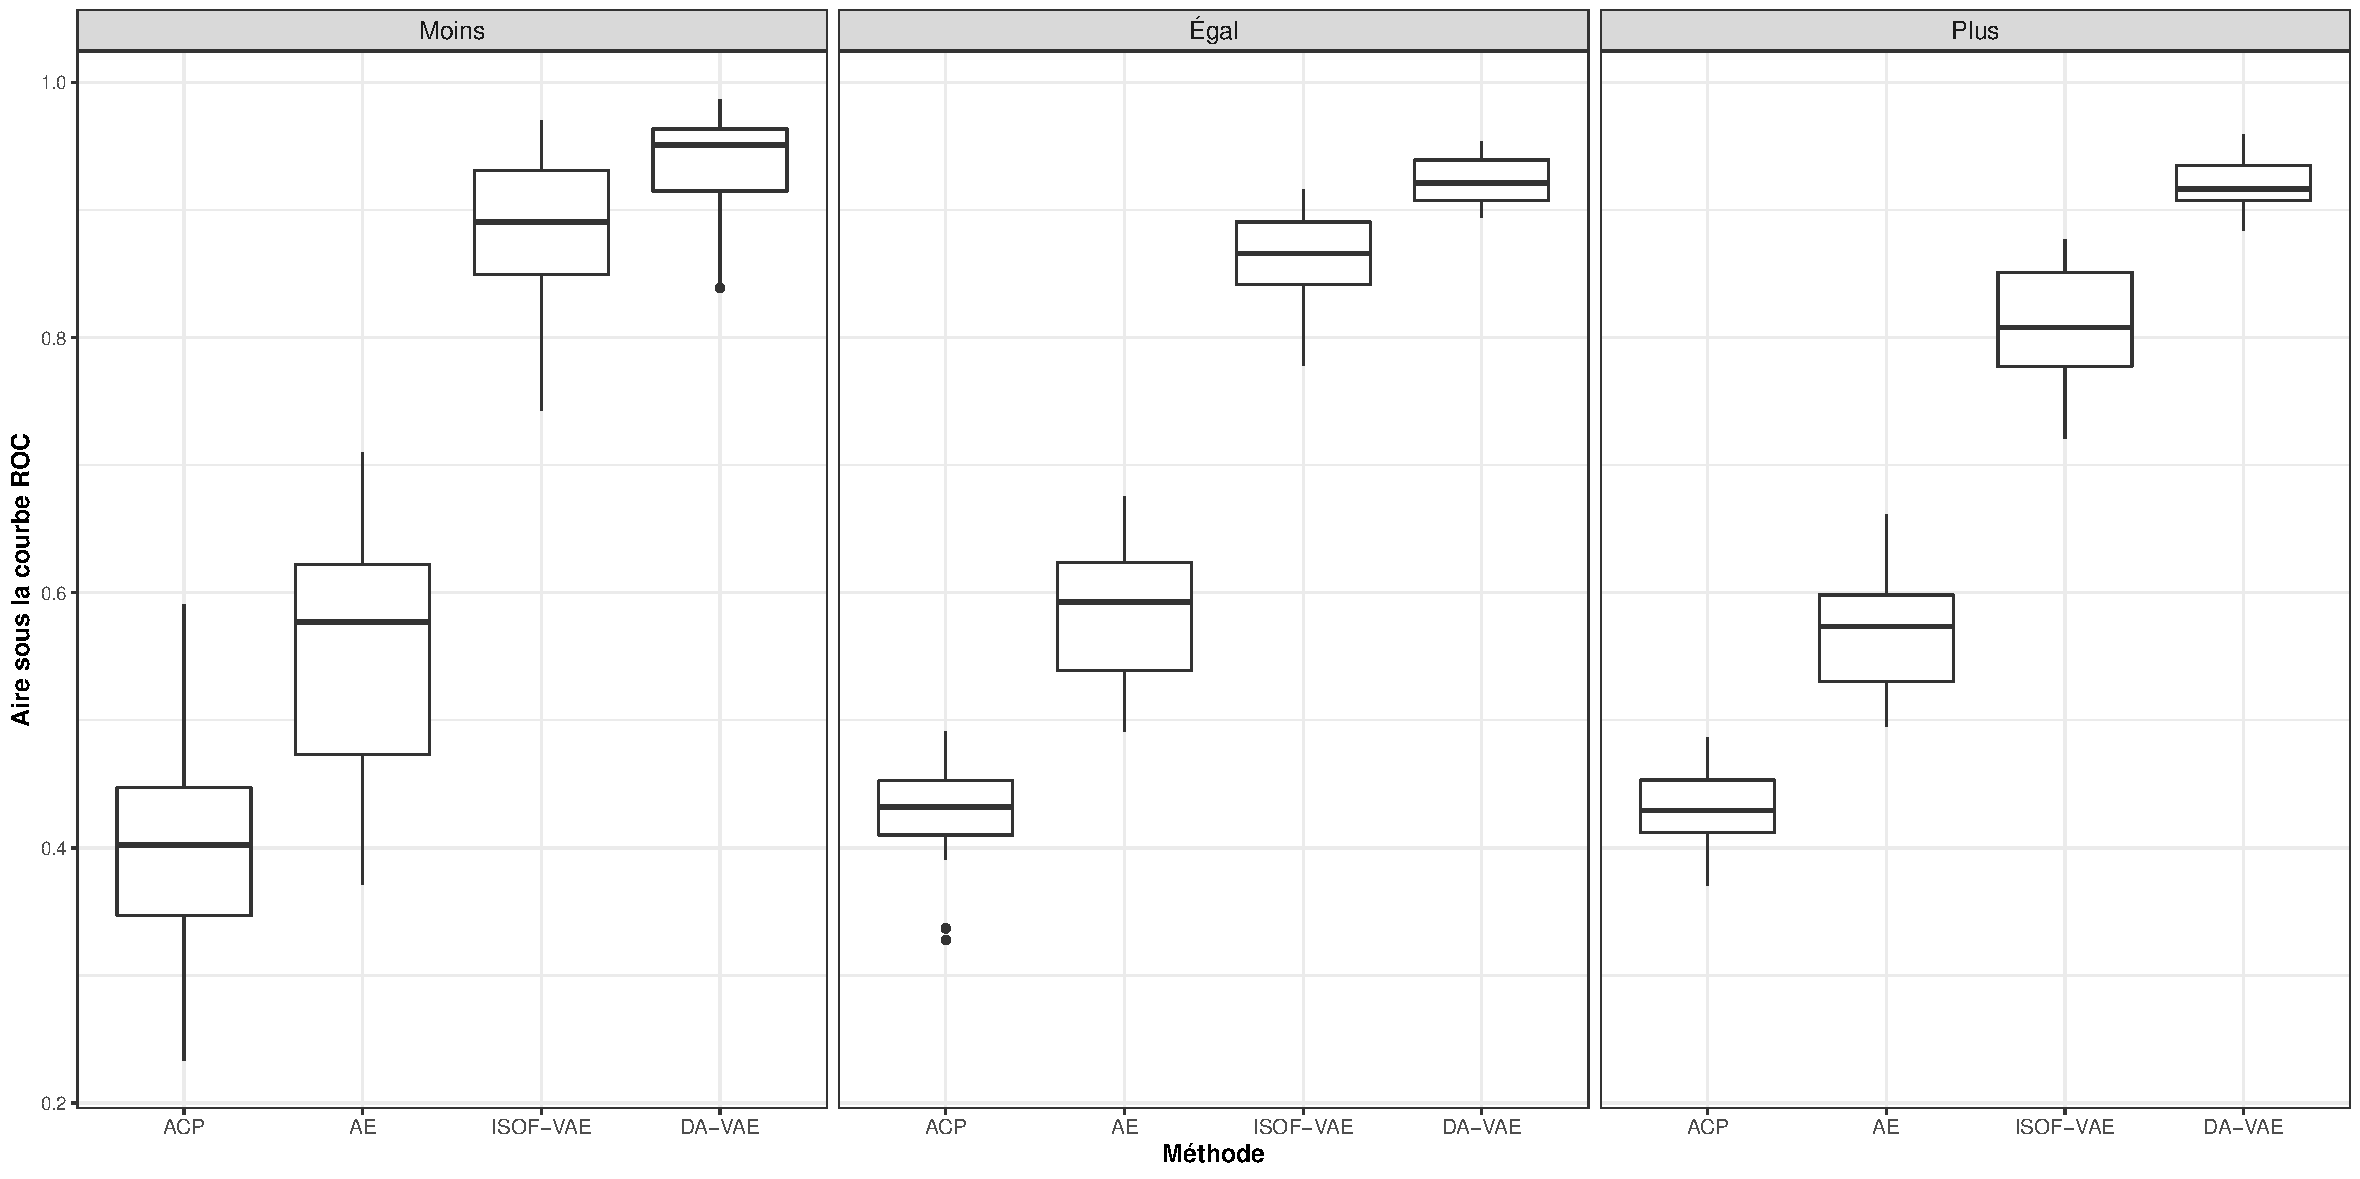
\includegraphics[width=8cm]{../rapports/images/images_boxplots/auc_cars.pdf}
		
	\end{frame}

	\begin{frame}
		\frametitle{Résultats -  ImageNet}
		
		Résultats sur les anomalies (jaunes) et les observations "normales" (mauves) du jeu de données $\mathcal{X^*}$.
		
		\vspace{0.5cm}
		
		\centering
		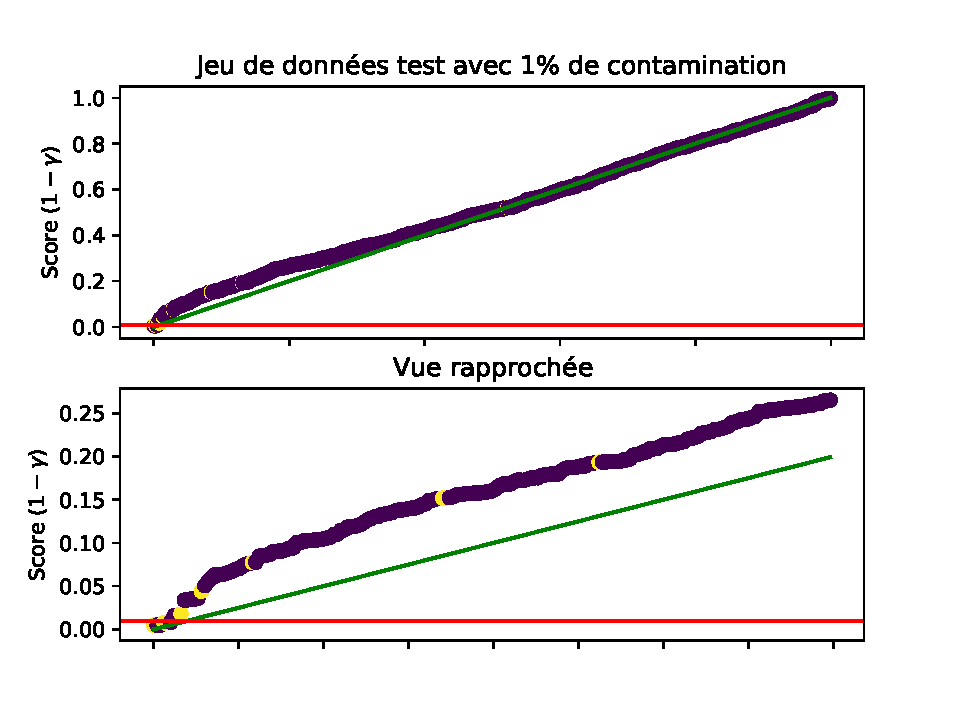
\includegraphics[width=4cm]{../rapports/images/images_davae/pvalues_scenario_cars_moins}
		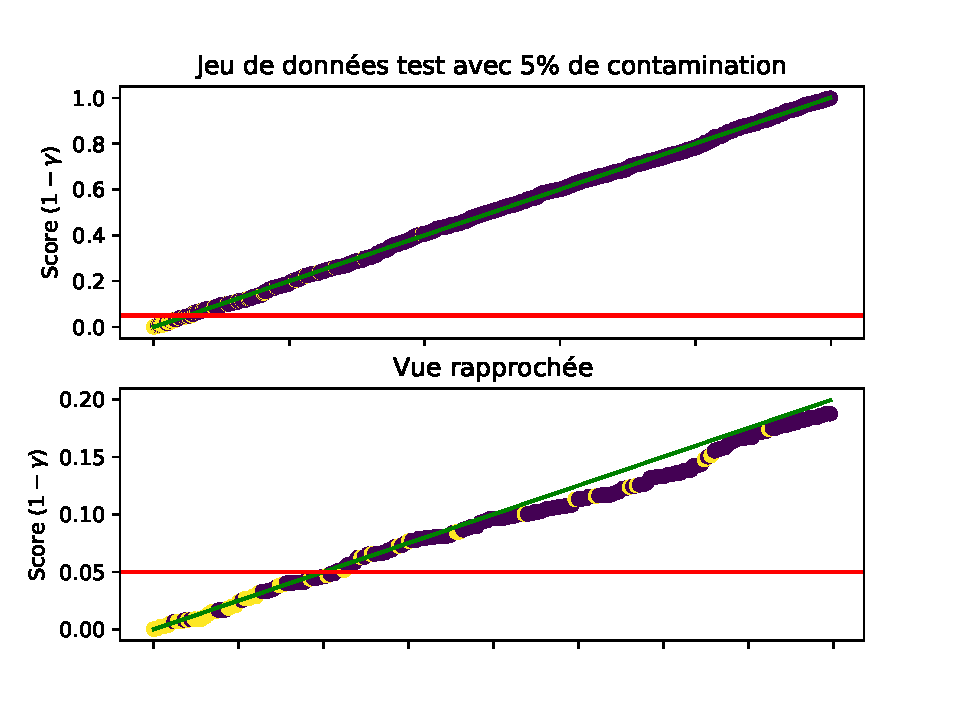
\includegraphics[width=4cm]{../rapports/images/images_davae/pvalues_scenario_cars_egal}
		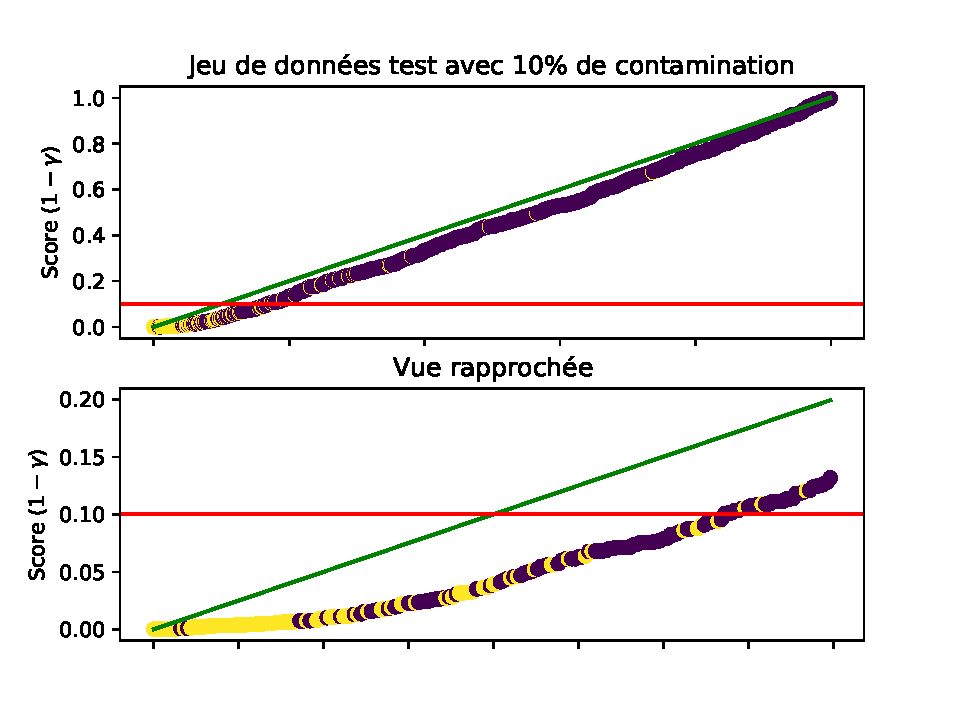
\includegraphics[width=4cm]{../rapports/images/images_davae/pvalues_scenario_cars_plus}
		
	\end{frame}

	\begin{frame}
		\frametitle{Analyse des résultats}
		
		Si on regarde quelques résultats des méthodes basées sur la reconstruction, on remarque que le contenu de l'image n'est pas le facteur déterminant dans la détection d'anomalie.
		
		\vspace{0.5cm}
		
		\begin{figure}
			\centering
			\begin{minipage}{.45\textwidth}
				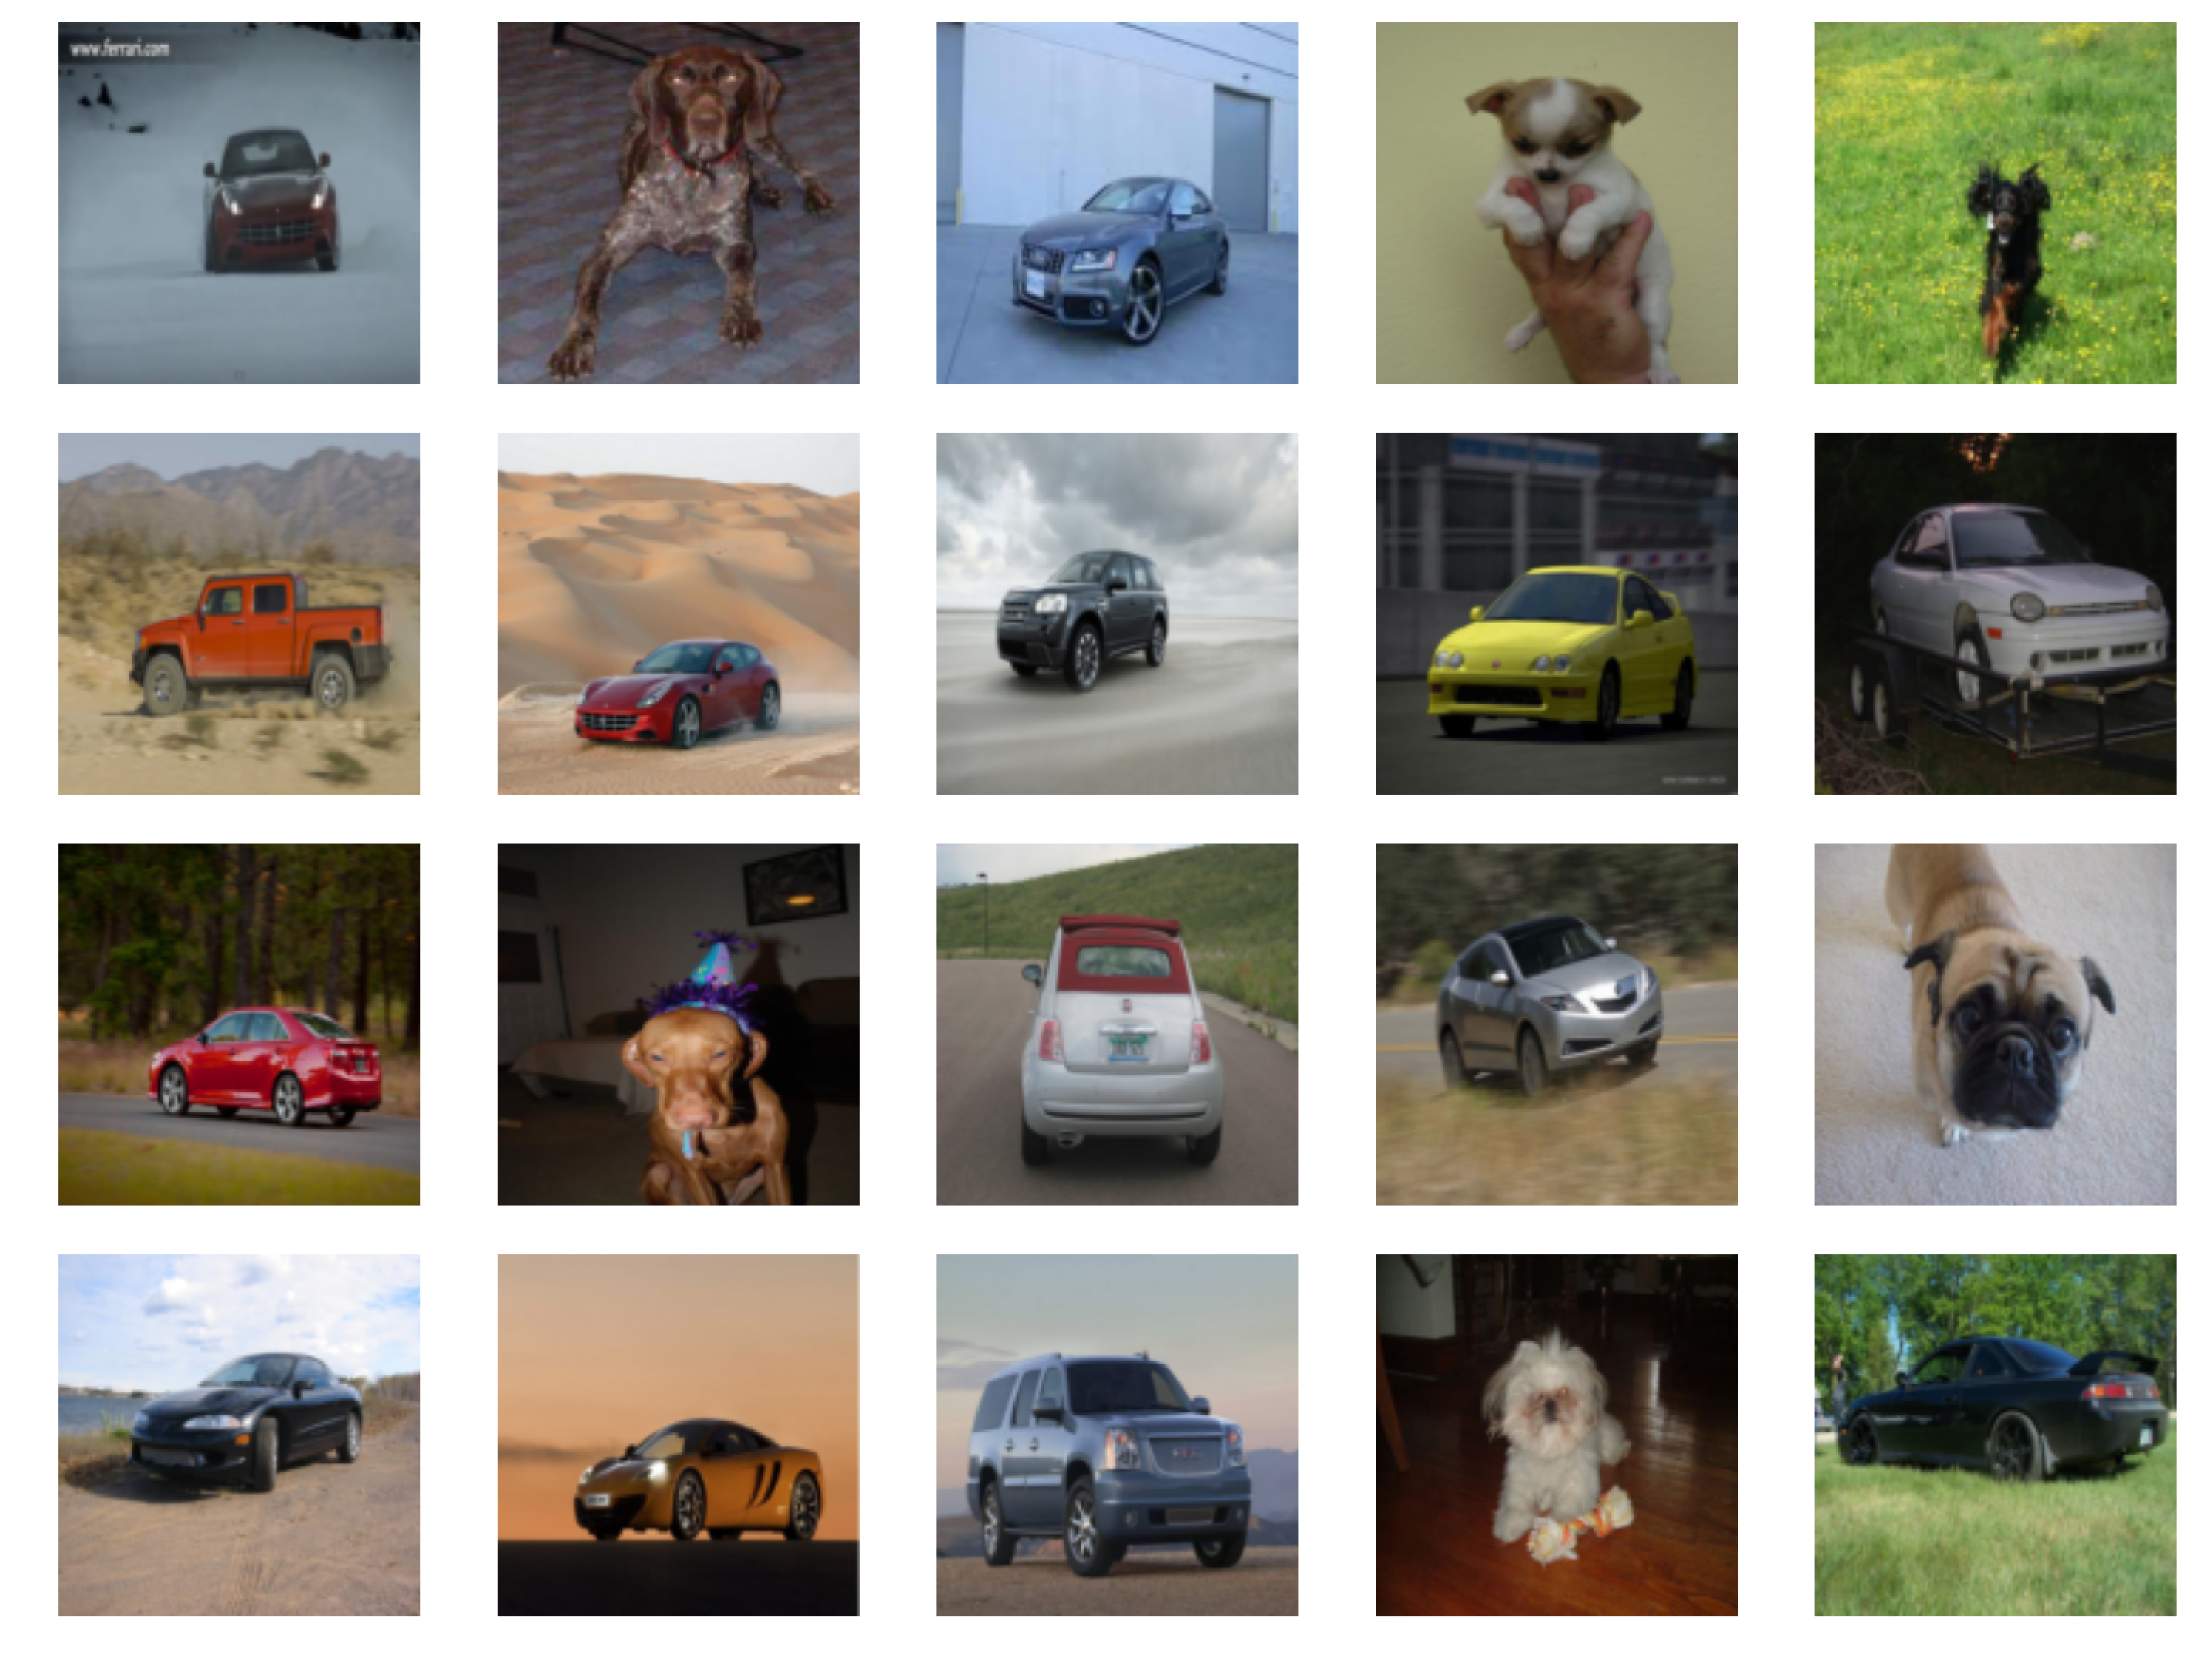
\includegraphics[width=5cm]{../rapports/images/smallest_errors}
				\caption{Bonnes reconstructions}
			\end{minipage}\hfill
			\begin{minipage}{.45\textwidth}
				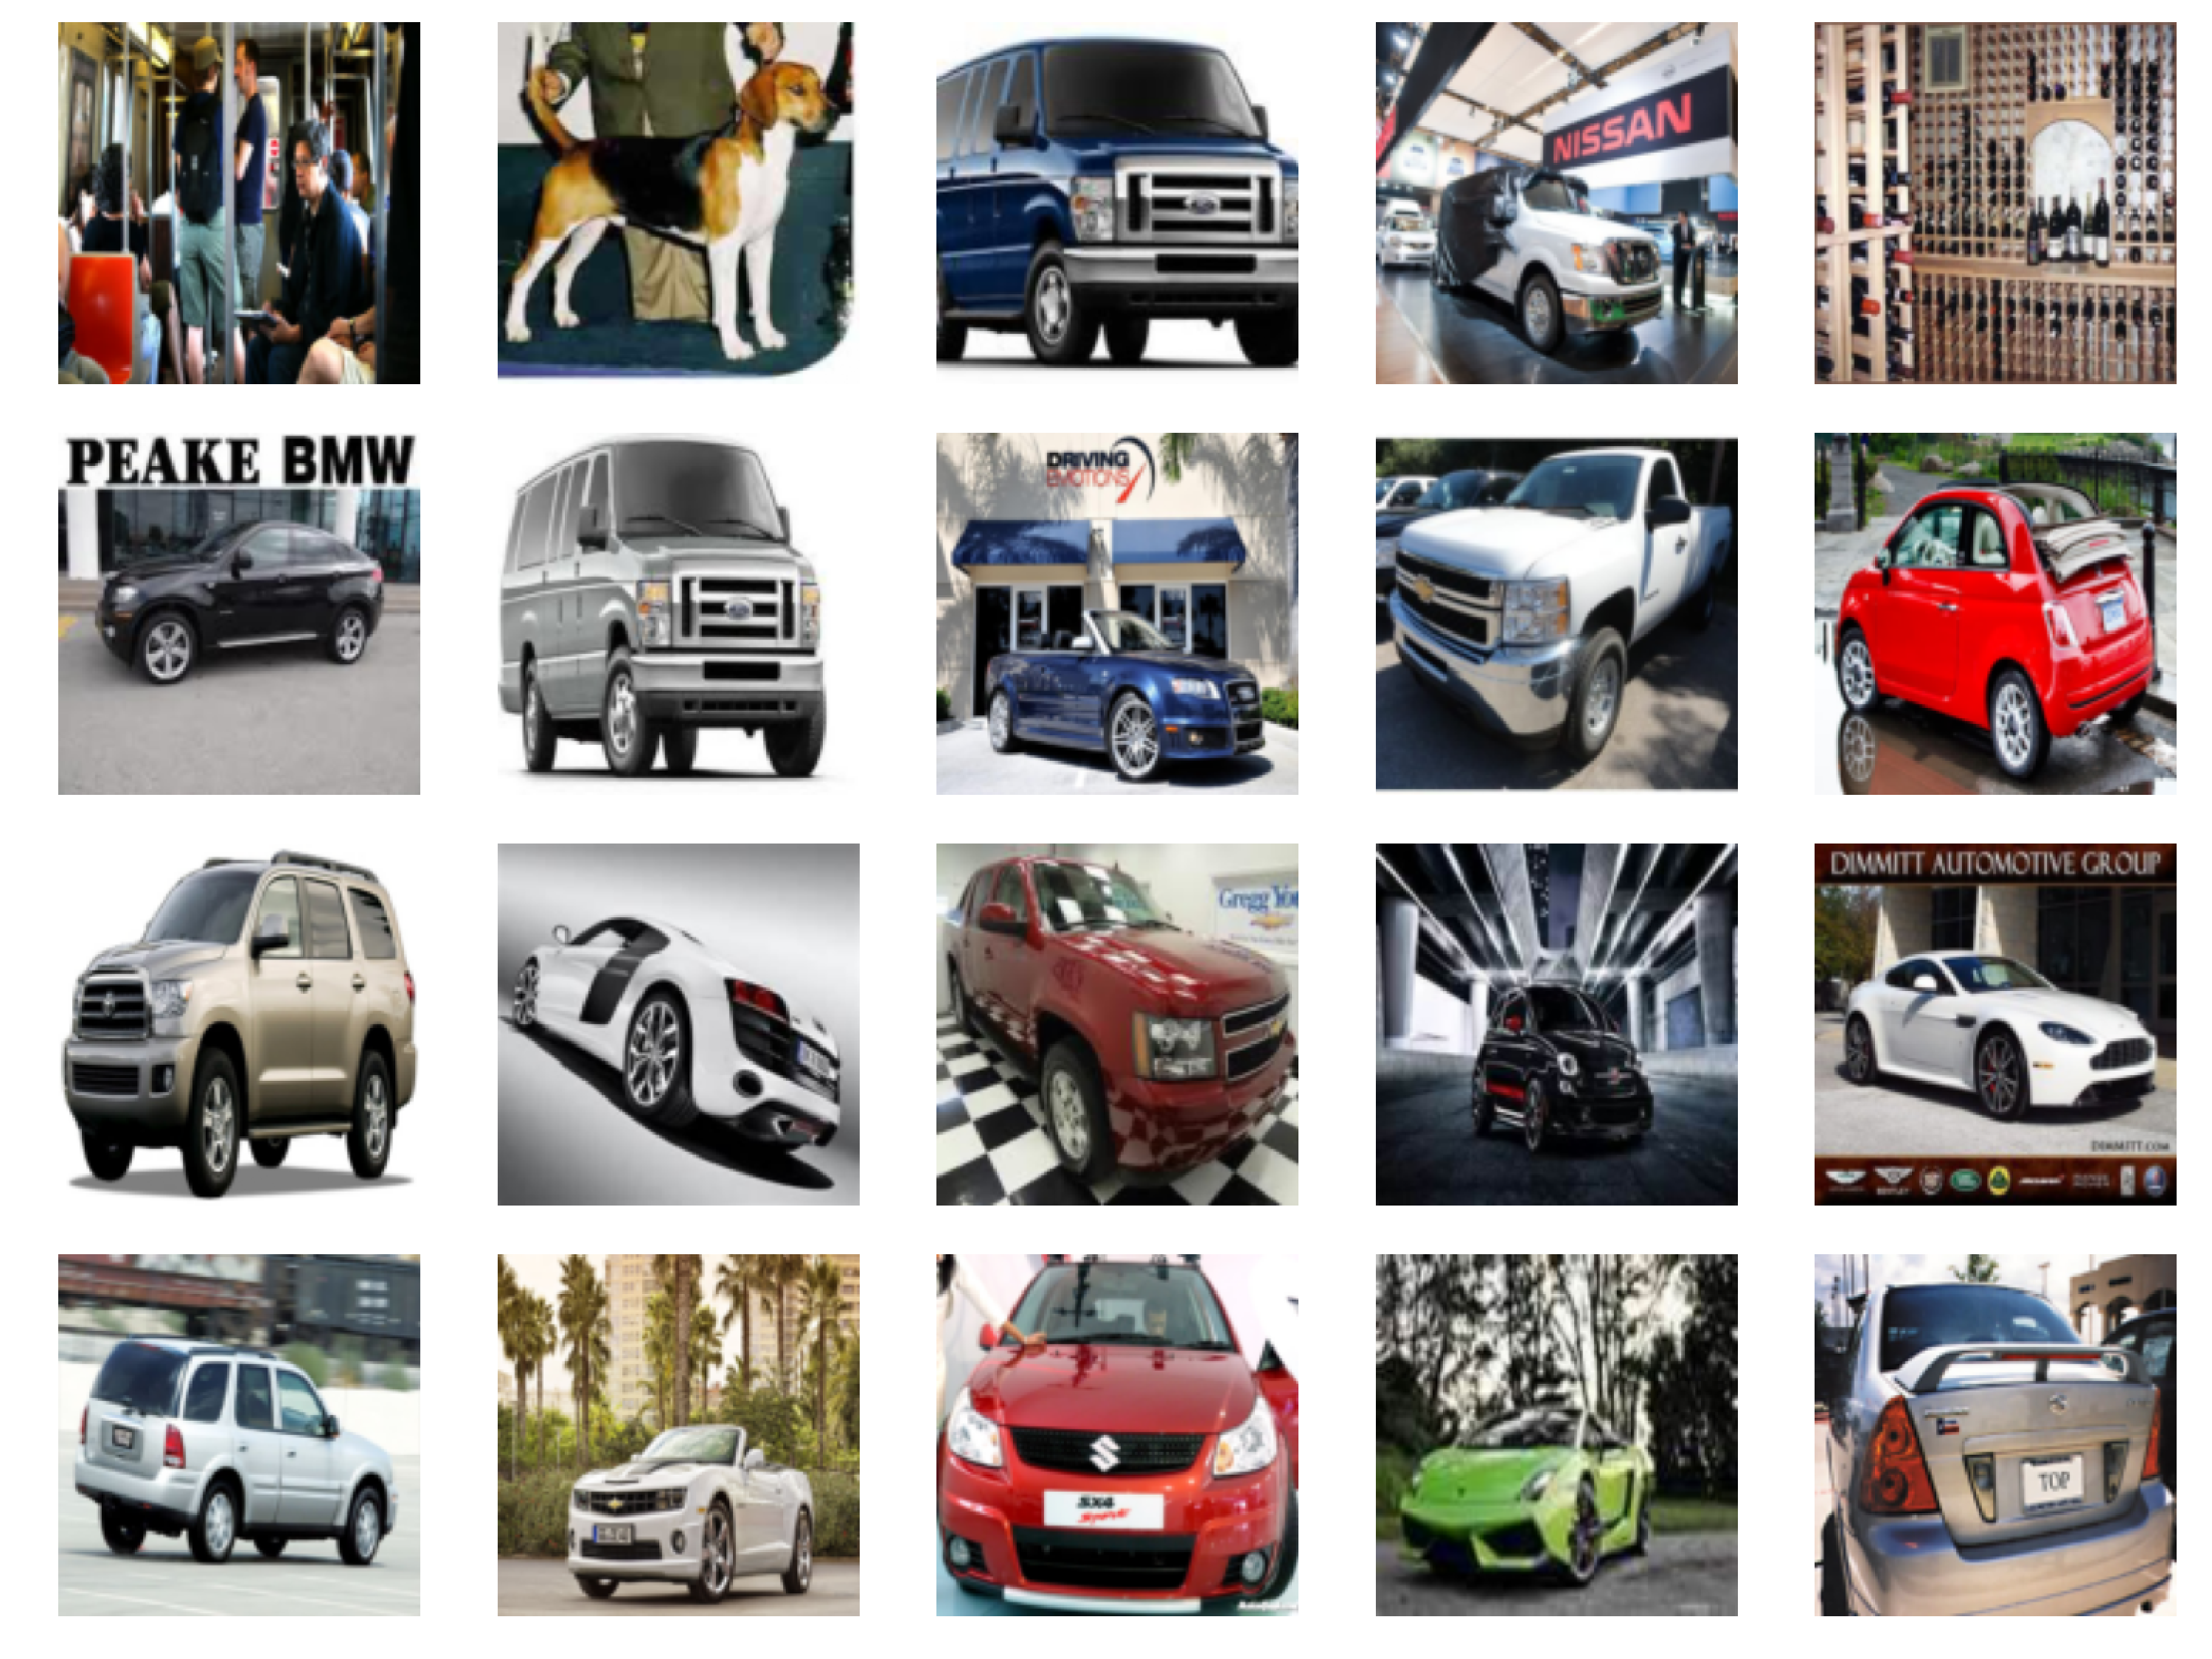
\includegraphics[width=5cm]{../rapports/images/biggest_errors}
				\caption{Mauvaises reconstructions}
			\end{minipage}
		\end{figure}
		
		
	\end{frame}

	\begin{frame}
		\frametitle{Analyse des résultats}
		
		Si on regarde notre modèle, la représentation latente semble bien différente entre les anomalies et les observations "normales".
		
		\vspace{0.5cm}
		
		\begin{figure}
			\centering
			\begin{minipage}{.45\textwidth}
				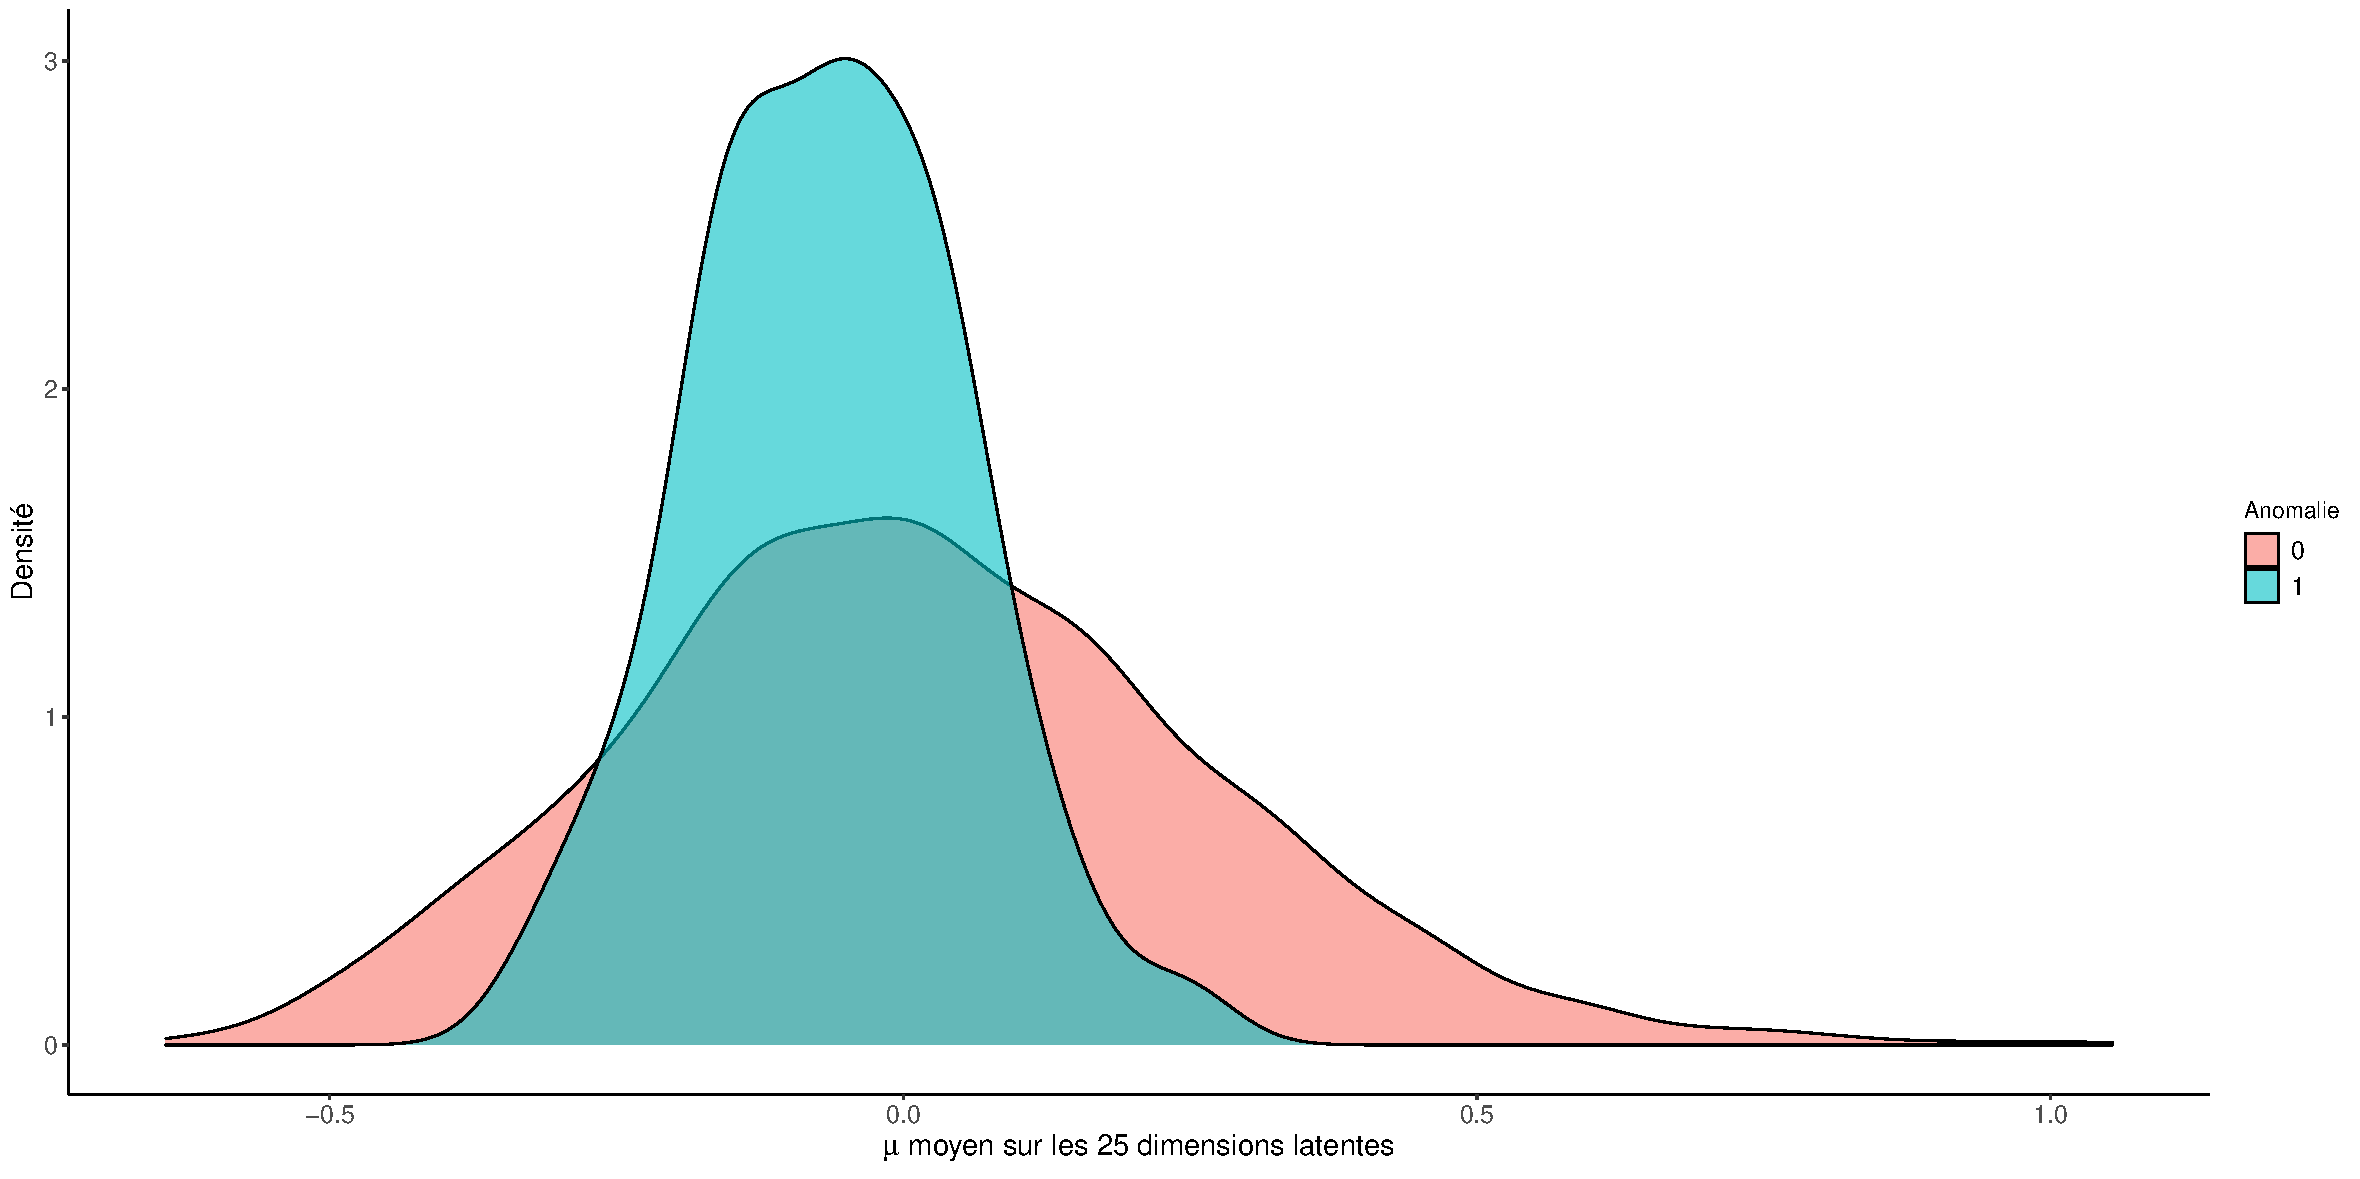
\includegraphics[width=5cm]{../rapports/images/latent_stats/plot_mu}
				\caption{Distribution des $\mu$}
			\end{minipage}\hfill
			\begin{minipage}{.45\textwidth}
				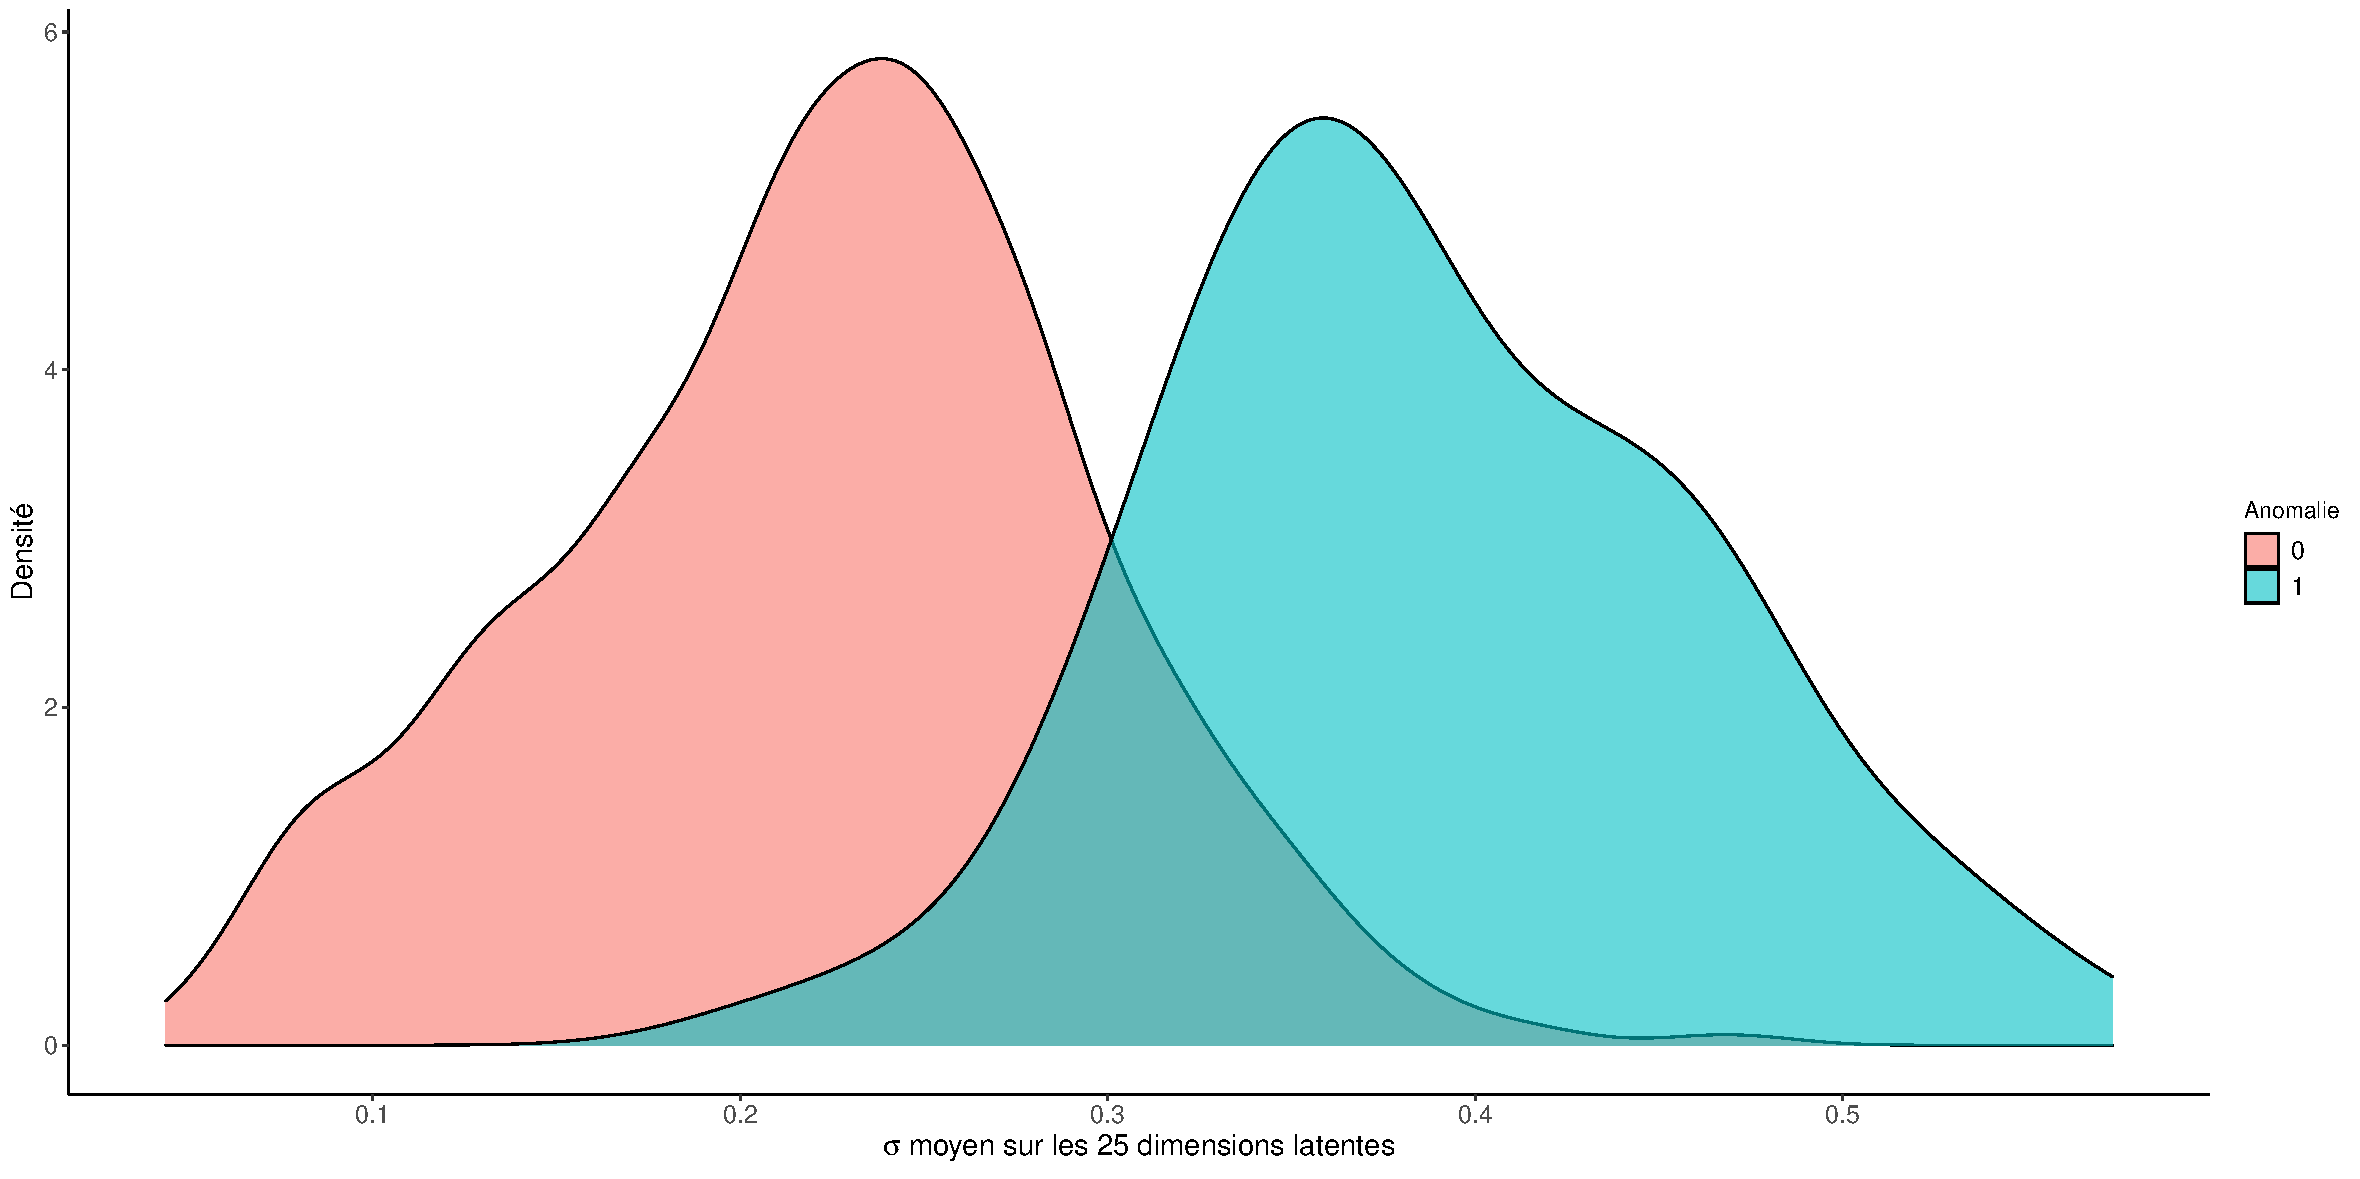
\includegraphics[width=5cm]{../rapports/images/latent_stats/plot_sigma}
				\caption{Distribution des $\sigma$}
			\end{minipage}
		\end{figure}
		
	\end{frame}

	\begin{frame}
		\frametitle{Analyse des résultats}
		
		Si on regarde notre modèle, la représentation latente semble bien différente entre les anomalies et les observations "normales".
		
		\vspace{0.5cm}
		
		\begin{figure}
			\centering
			\begin{minipage}{.45\textwidth}
				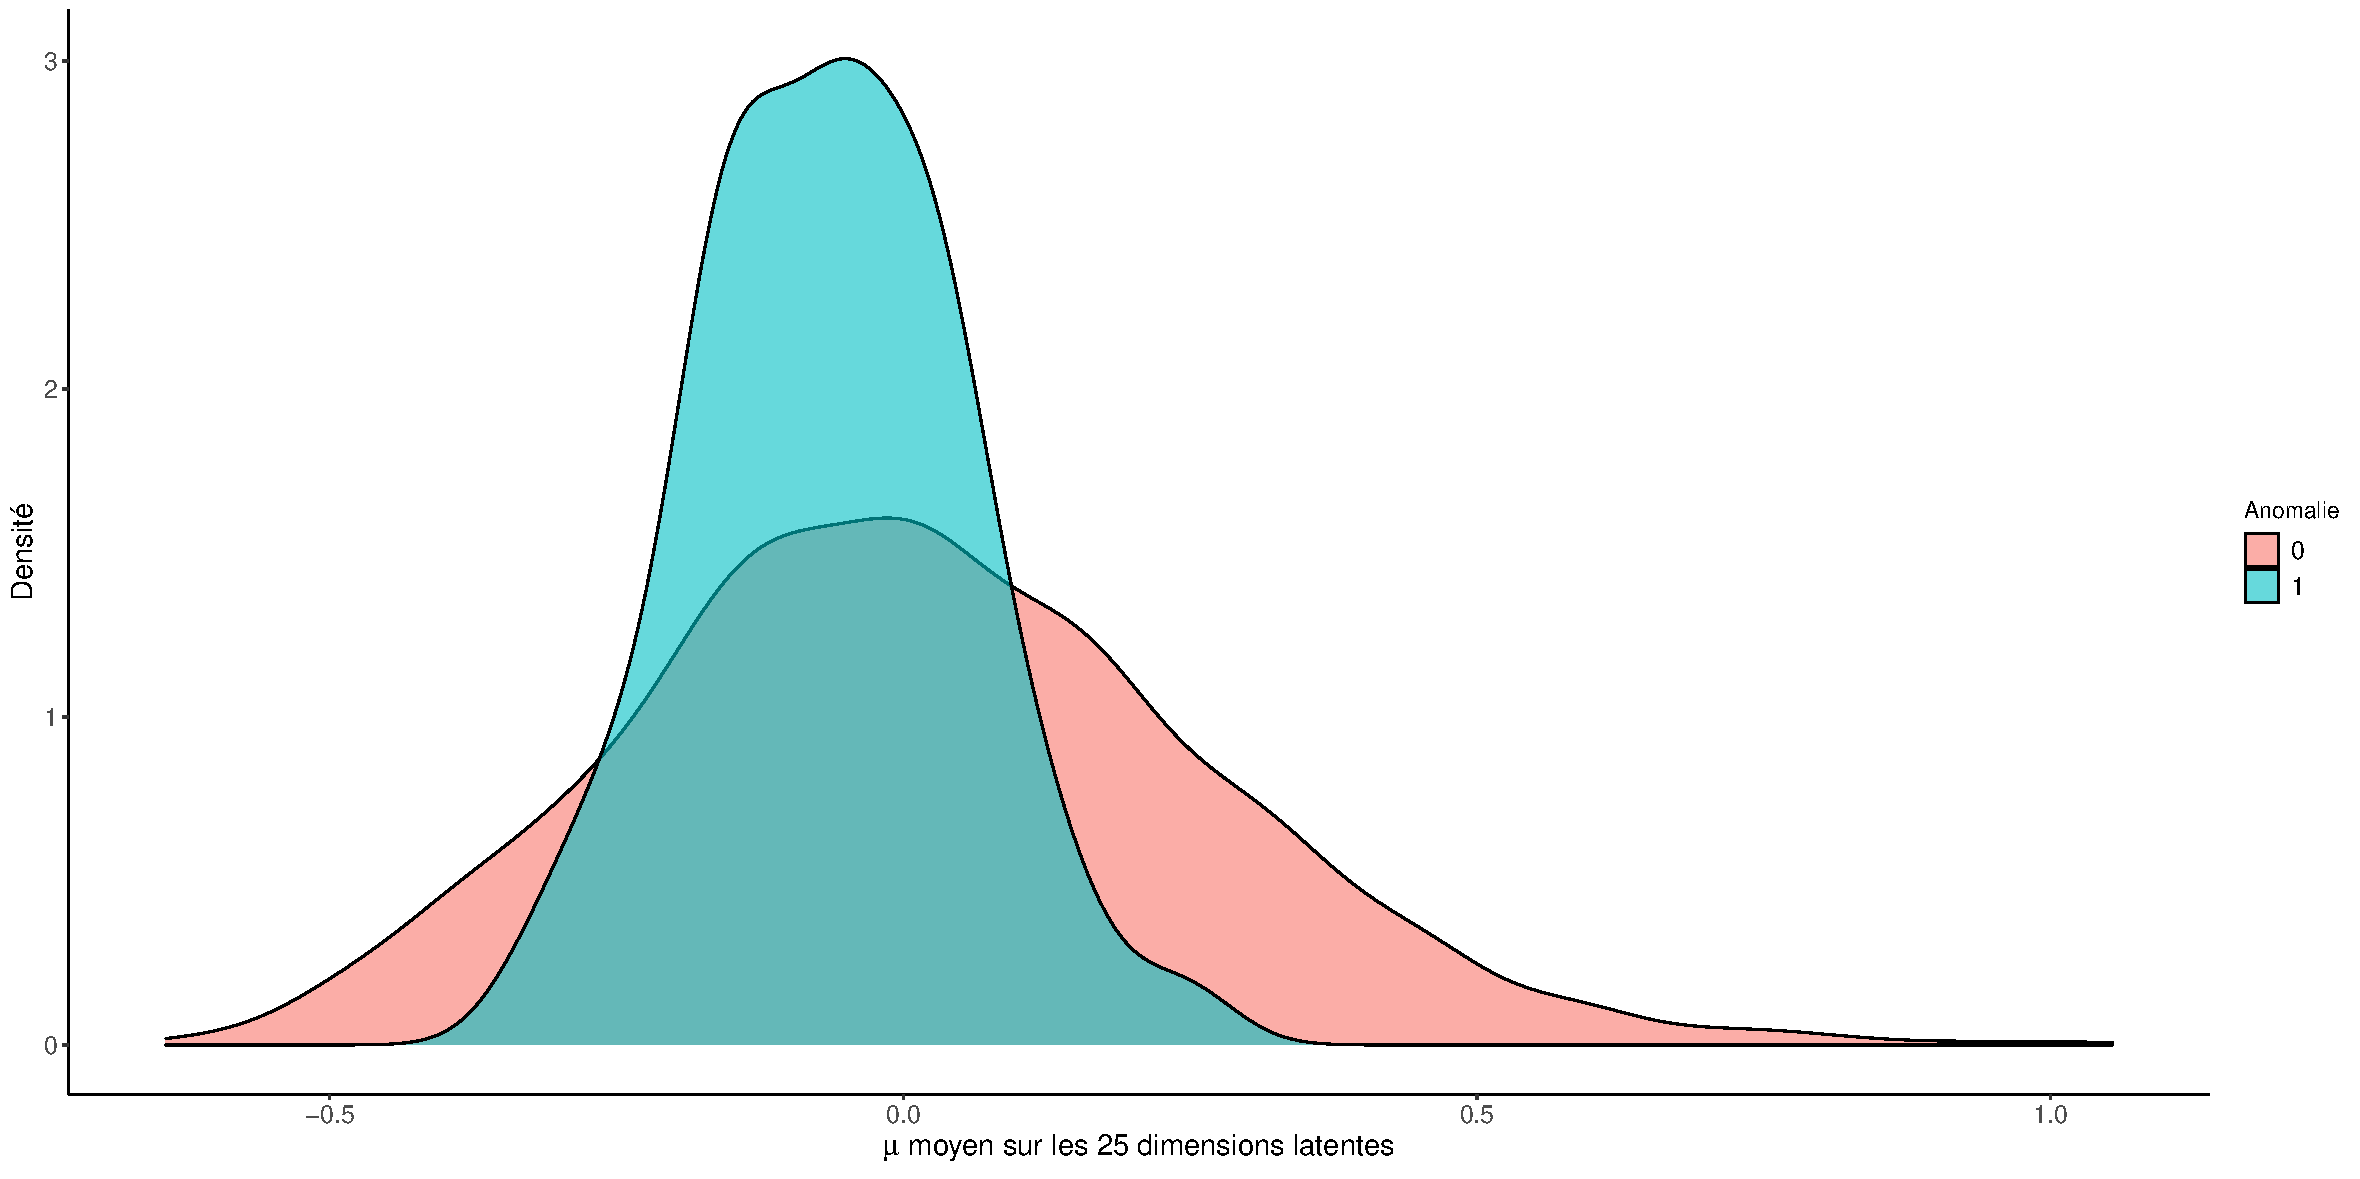
\includegraphics[width=5cm]{../rapports/images/latent_stats/plot_mu}
				\caption{Distribution des $\mu$}
			\end{minipage}\hfill
			\begin{minipage}{.45\textwidth}
				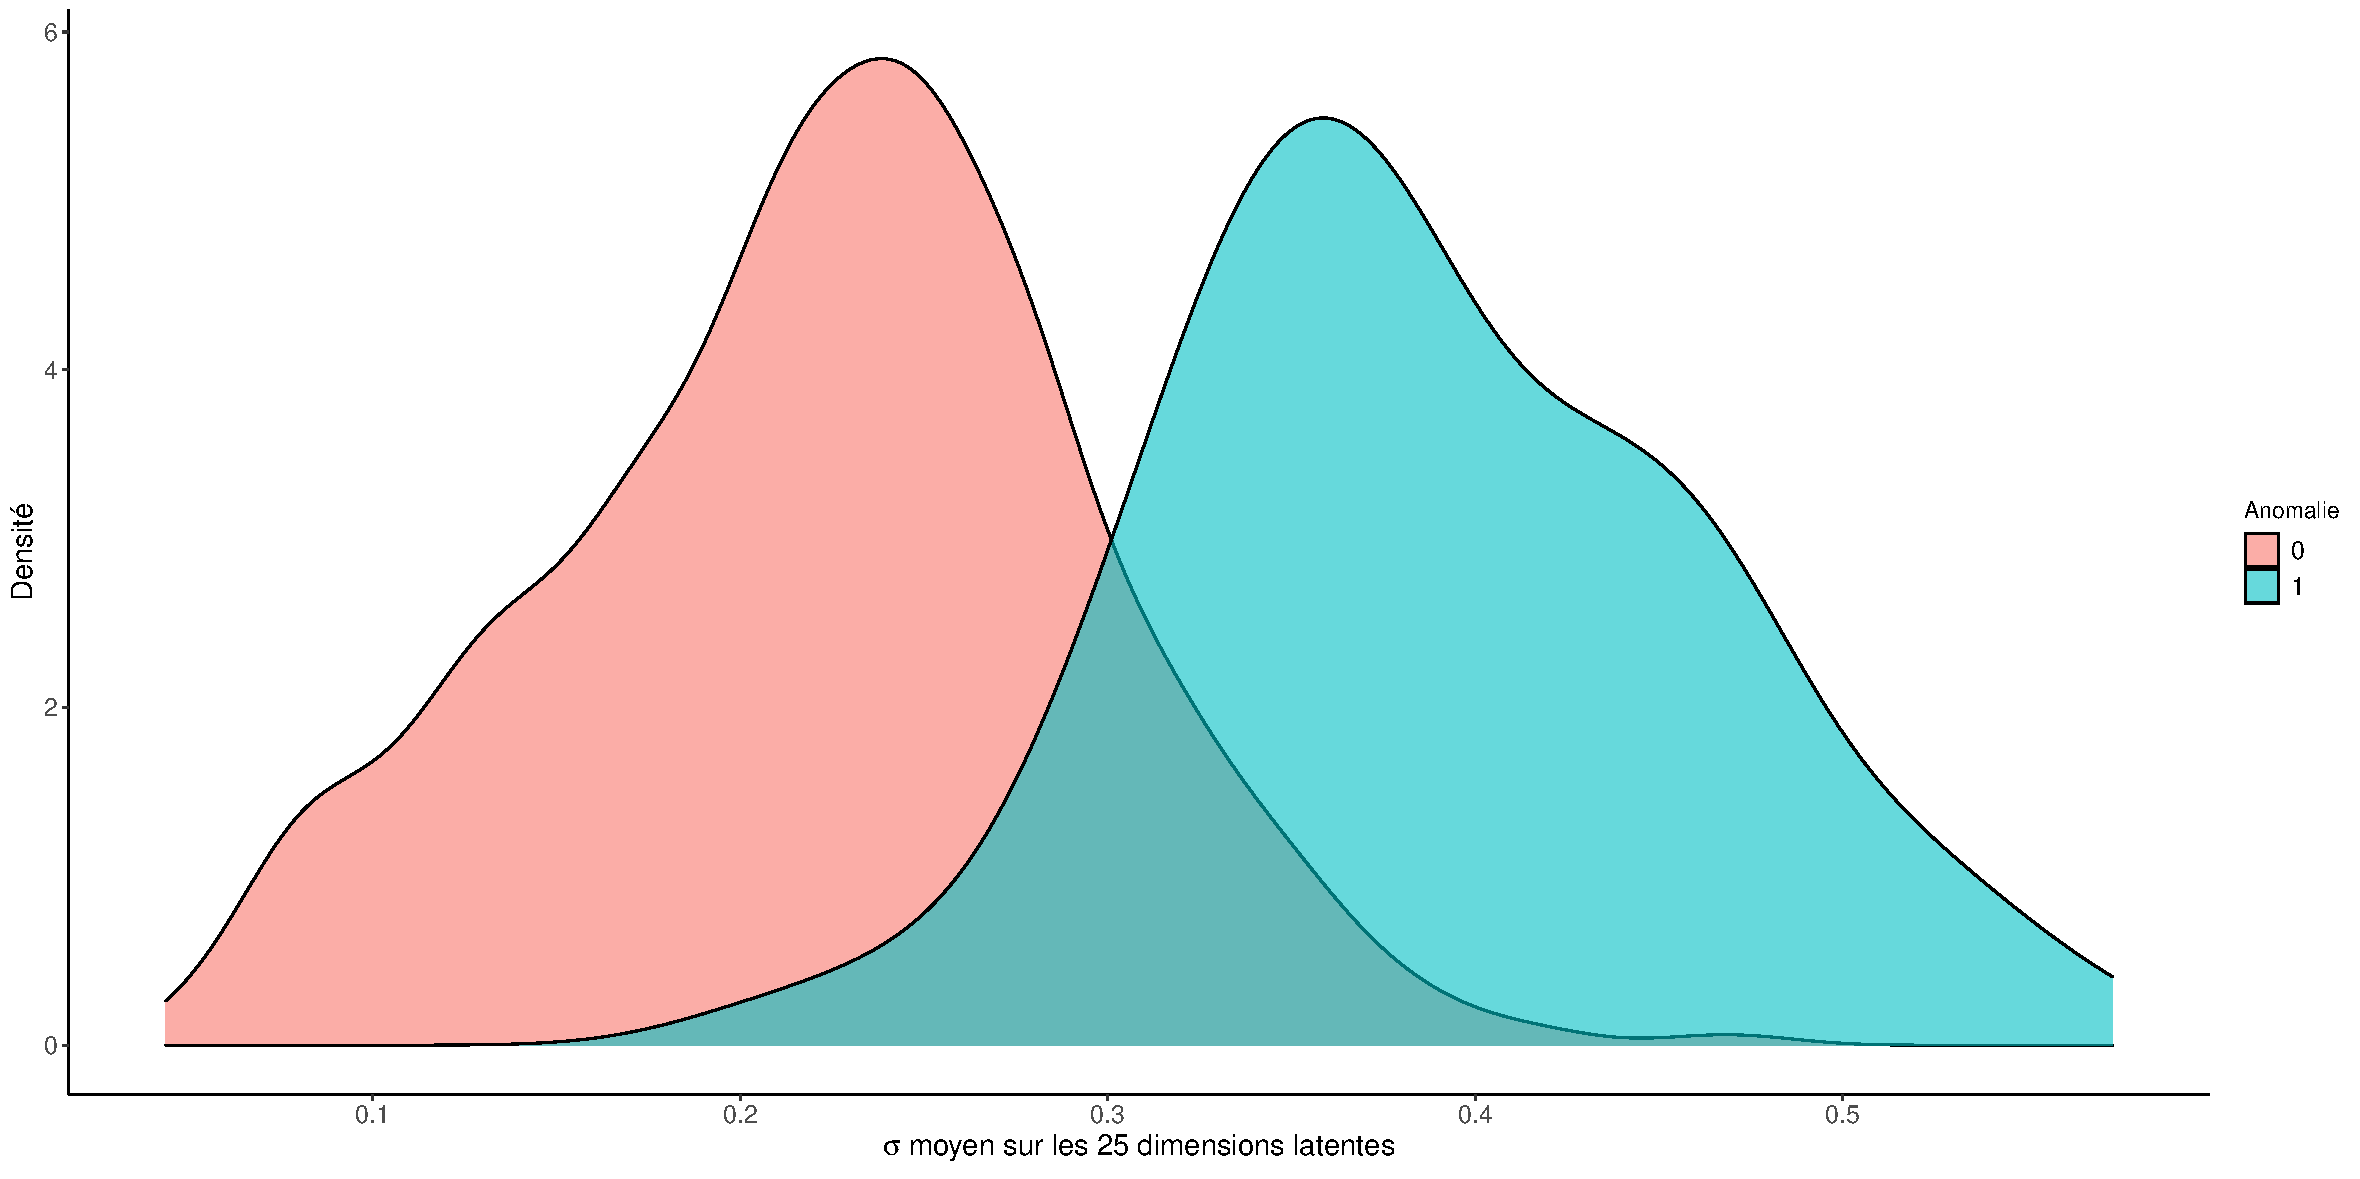
\includegraphics[width=5cm]{../rapports/images/latent_stats/plot_sigma}
				\caption{Distribution des $\sigma$}
			\end{minipage}
		\end{figure}
		
	\end{frame}
	
	\section{Conclusion}
	
	\begin{frame}
		\frametitle{Exemple d'application}
		
		On pourrait imaginer un exemple d'application pour nettoyer un jeu de données qui peut contenir des images abérantes.
		
		\begin{figure}
			\centering
			\begin{minipage}{.45\textwidth}
				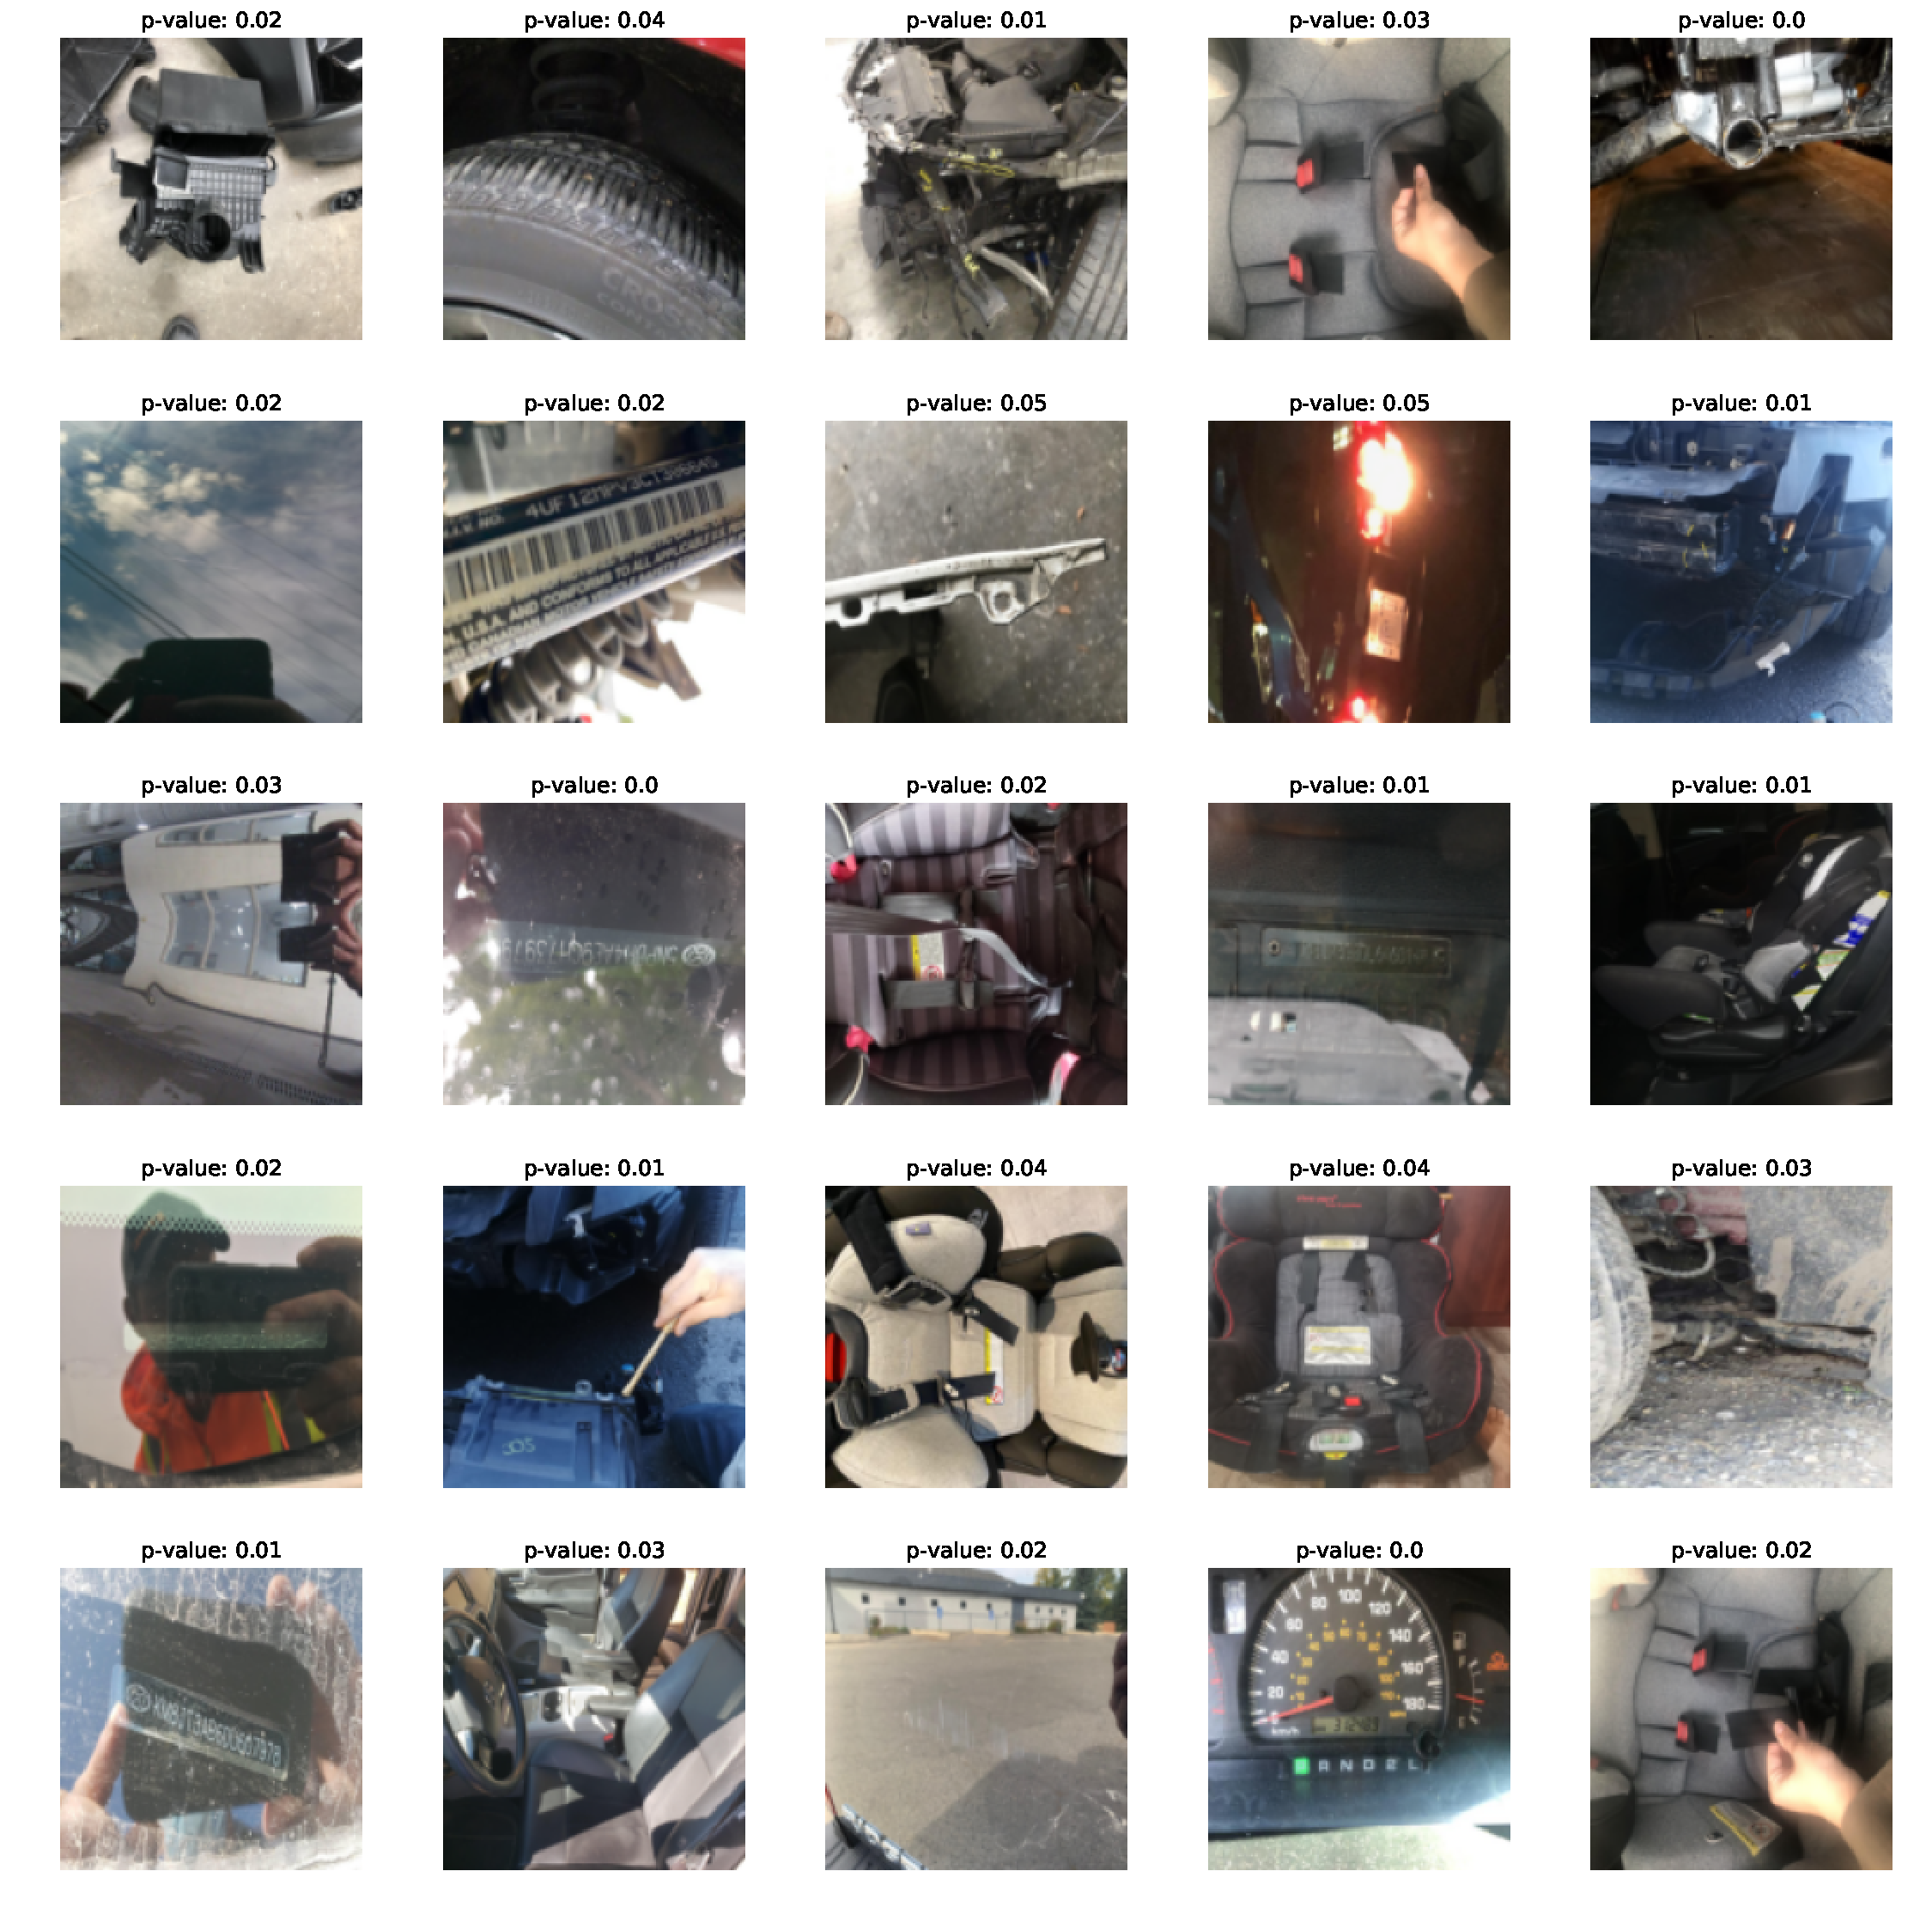
\includegraphics[width=5cm]{images/bad.pdf}
				\caption{Exemples avec $\gamma > (1 - \alpha)$}
			\end{minipage}\hfill
			\begin{minipage}{.45\textwidth}
				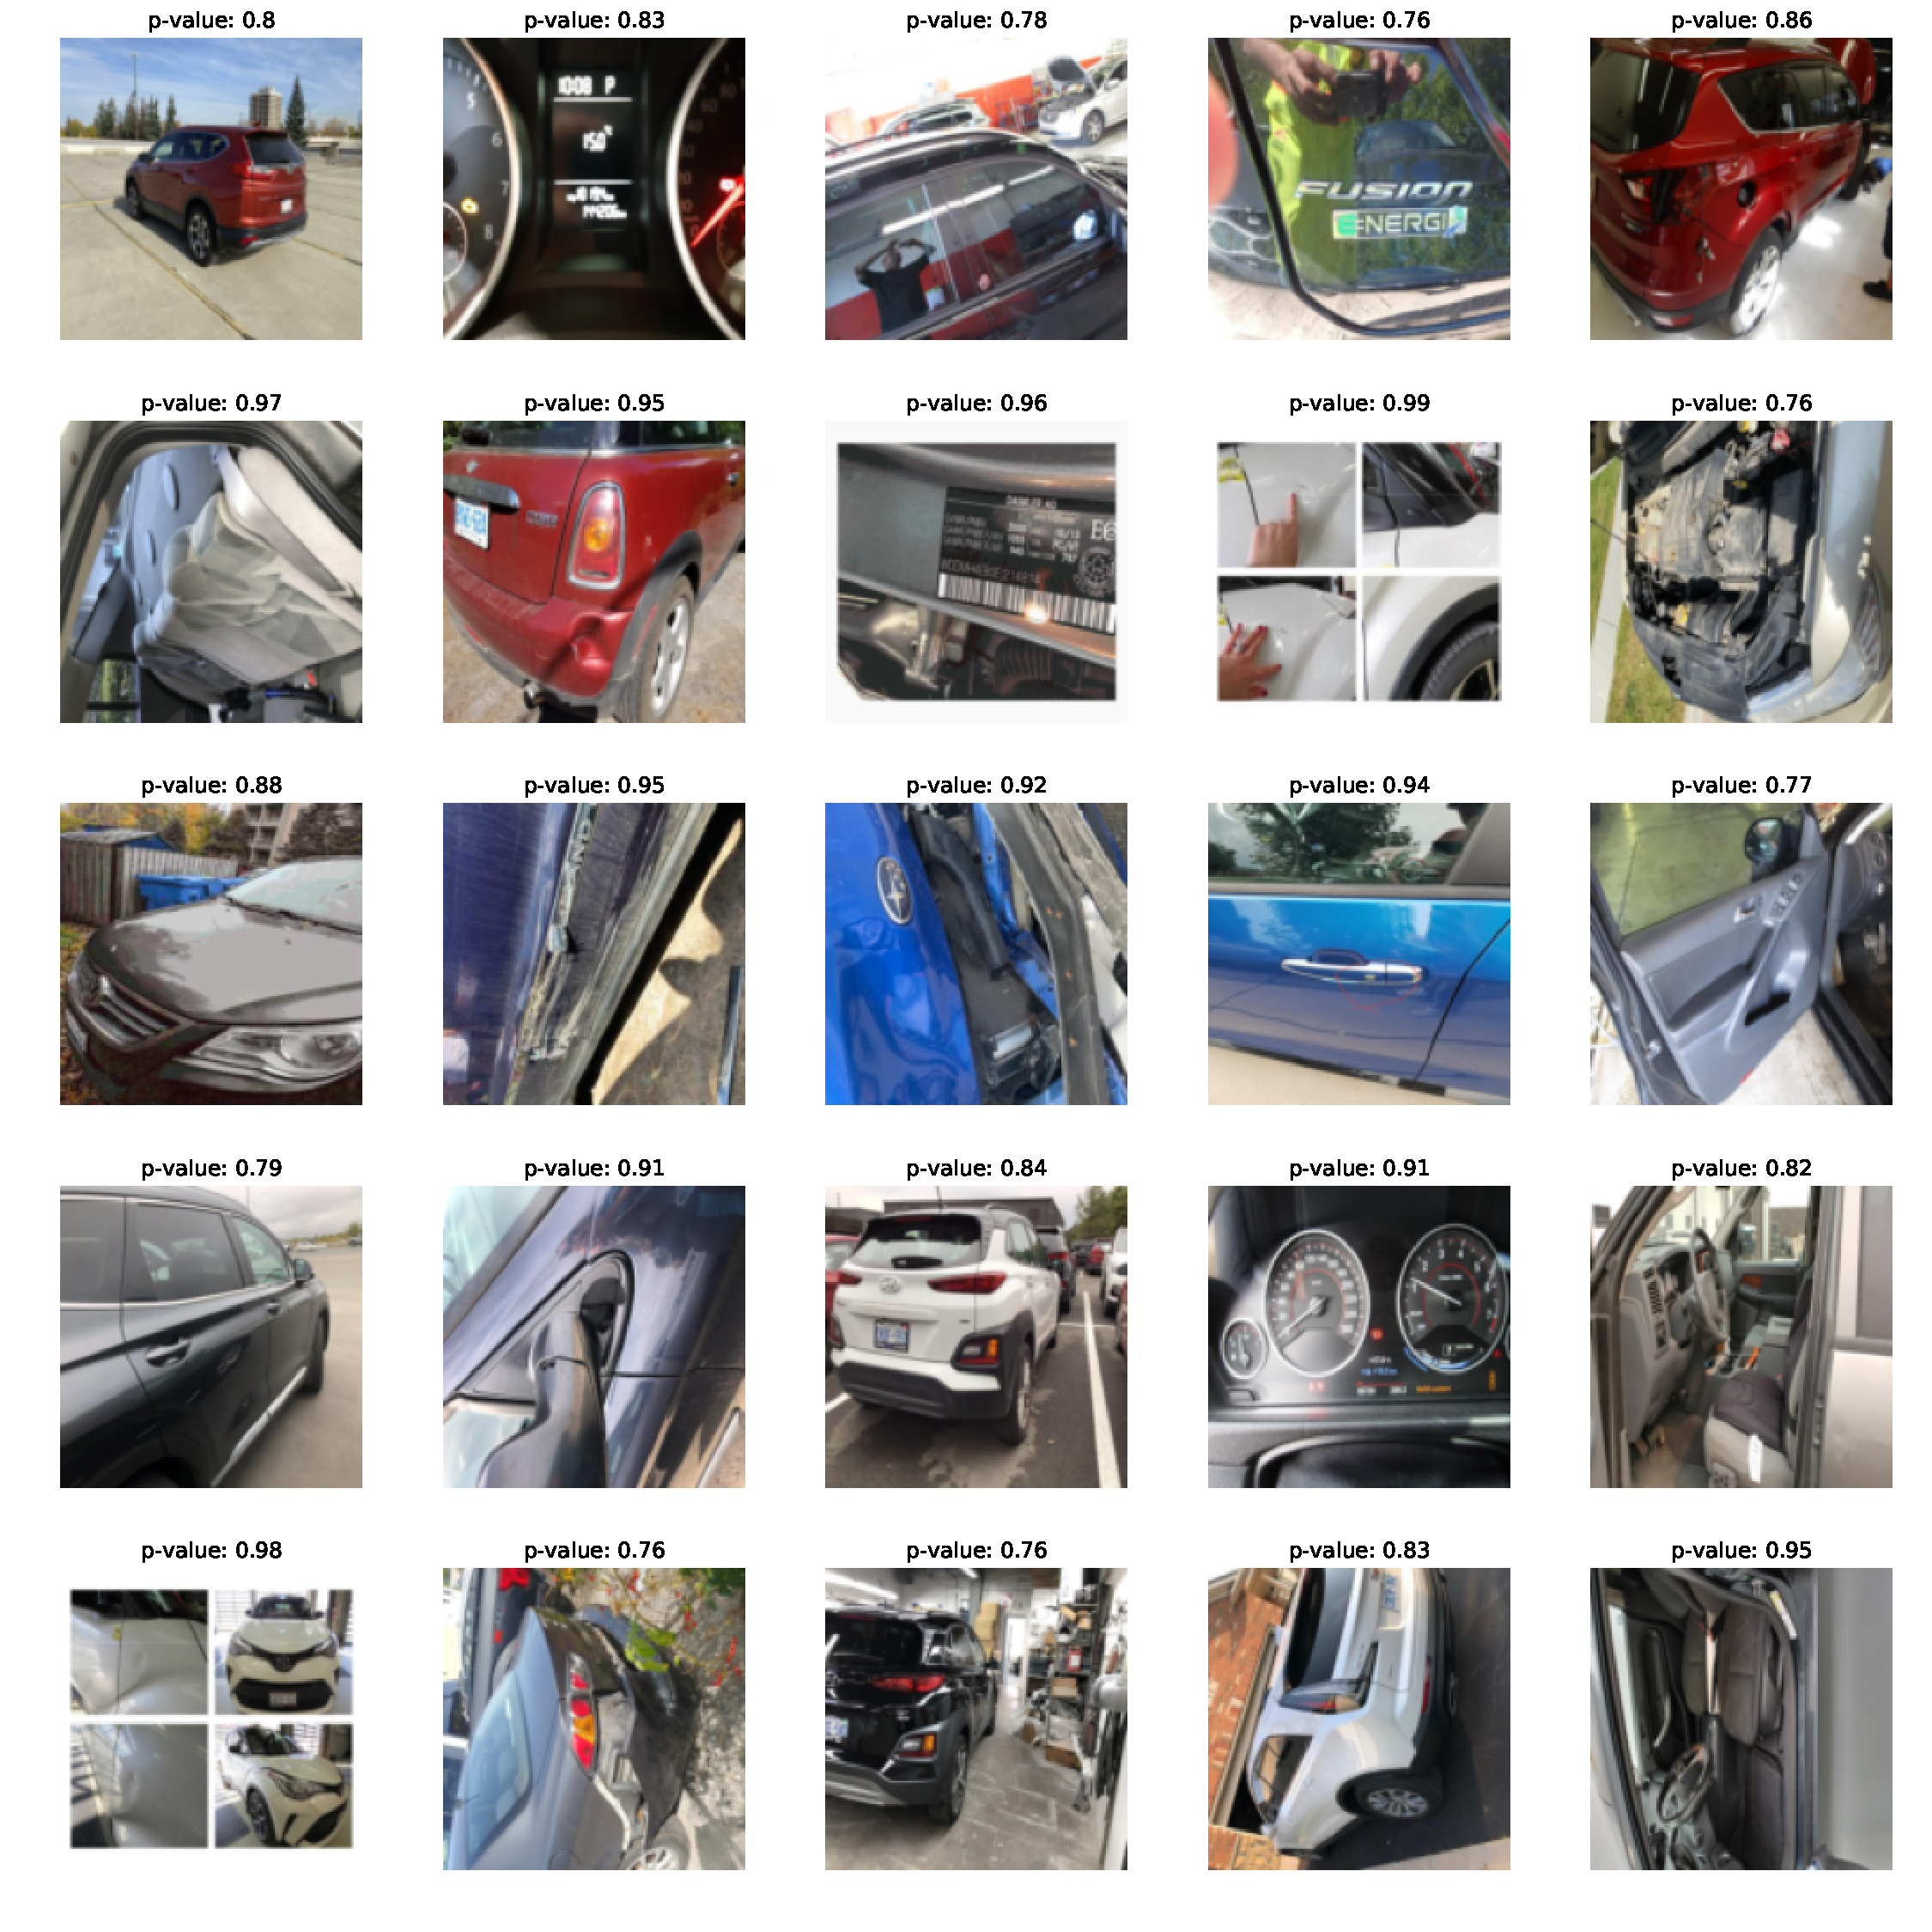
\includegraphics[width=5cm]{images/good.pdf}
				\caption{Exemples avec $\gamma \le (1 - \alpha)$}
			\end{minipage}
		\end{figure}
		
	\end{frame}
	
	\begin{frame}
		\frametitle{Points à retenir}
		
		\begin{itemize}
			\item Pour des images complexes, les autoencodeurs permettent de bien capturer l'information des données et sont utiles dans un contexte de détection d'anomalies.
			\item L'utilisation des représentations latentes permet de mieux modéliser le contenu d'une image, contrairement à la reconstruction qui peut être davantage affectée par la complexité variante des images dans un jeu de données.
			\item Pour obtenir une représentation latente qui répond à certains objectifs, les $\beta$-VAE sont des modèles difficiles à entraîner et à ajuster (beaucoup d'essaies-erreurs).
		\end{itemize}
	
	\end{frame}

	\begin{frame}
		\frametitle{Aspects à explorer}
		
		\begin{itemize}
			\item Voir si d'autres lois de probabilité, autre que la $N(0,I)$, pourraient être utilisées comme loi \textit{a priori} pour régulariser la représentation latente.
			\item Mieux comprendre les comportements possibles de la représentation latente (les 2 scénarios expliqués dans la méthodologie).
		\end{itemize}
		
	\end{frame}
	
	
	\begin{frame}
		\frametitle{Bibliographie}
		\bibliography{../rapports/bibliography.bib}
	\end{frame}

	\appendix
	\section{Appendice}
	
	\begin{frame}[label=supplemental]
		\frametitle{Score d'anomalie basé sur la reconstruction}
		Pour les méthodes PCA et AE, nous avons appliqué une approche de détection d'anomalie basée sur la capacité de reconstruire l'entrée $x$ avec un niveau de filtration $\alpha$:
		
		$$
		l(x^{*(j)}, \hat{x}^{*(j)}) > t_{1-\alpha}(L(\mathcal{X}, \hat{\mathcal{X}}))
		$$
		
		On suppose toujours que $\alpha$ est égale au niveau de contamination dans $\mathcal{X^*}$, soit $p^*$.
		
	\end{frame}
	
	\begin{frame}
		\frametitle{Détails sur ISOF-VAE}
		
		\centering
		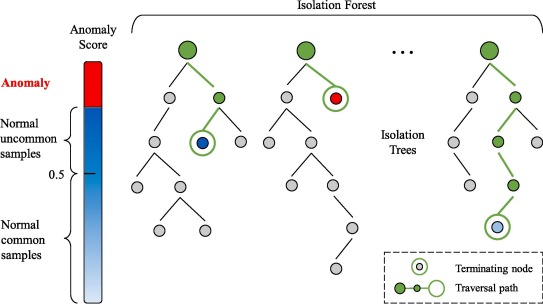
\includegraphics[width=7cm]{images/isolation-forest}
		\blfootnote{Image tirée de \cite{CHEN2020101139}}
		
	\end{frame}
	
	
	\begin{frame}
		\frametitle{Détails sur ISOF-VAE}
		
		Pour la méthode basée sur les Isolation Forest, nous avons utilisé le score d'anomalie calculé par l'algorithme :
		
		\begin{itemize}
			\item $S$: score d'anomalie calculé par l'algorithme
			\item $S_{\mathcal{X}} = \{S^{(1)}, ..., S^{(n)}\}$
			\item $S^{'}_{\mathcal{X}}$: $S_{\mathcal{X}}$ ordonné en ordre croissant
			\item $S^*(x^{*(j)}) = \frac{rang_{S^{'}_{\mathcal{X}}}(S^{(j)})}{n}$
		\end{itemize}
		
		On suppose toujours que $\alpha$ est égale au niveau de contamination dans $\mathcal{X^*}$, soit $p^*$.
		
	\end{frame}


\end{document}